%============================================================
%  PROJETO DA DISCIPLINA - ANÁLISE E PROJETO ORIENTADO A OBJETOS
%  UTFPR - Câmpus Ponta Grossa
%  Compile with: pdflatex -> pdflatex
%============================================================
\documentclass[12pt, a4paper]{article}
\usepackage[utf8]{inputenc}
\usepackage[T1]{fontenc}
\usepackage[brazil]{babel}
\usepackage{times}
\usepackage[top=3cm, bottom=3cm, left=3cm, right=2cm]{geometry}
\setlength{\footskip}{1.5cm}
\usepackage{setspace}
\usepackage{indentfirst}
\usepackage{graphicx}
\usepackage{float}
\usepackage{caption}
\captionsetup{justification=raggedright, singlelinecheck=false}
\usepackage{booktabs}
\usepackage{array}
\usepackage{hyperref}
\usepackage{titlesec}
\usepackage{tocloft}
\usepackage{fancyhdr}
\usepackage{microtype}
\usepackage{parskip}
\usepackage{xcolor}
\hypersetup{colorlinks=true, linkcolor=black, urlcolor=blue, citecolor=black}
\setstretch{1.5}
\setlength{\parindent}{1.25cm}
\setlength{\parskip}{0pt}
 
% ---------- TÍTULOS DAS SEÇÕES ----------
\titleformat{\section}{\normalfont\bfseries\normalsize}{\thesection\quad}{0pt}{\MakeUppercase}
\titleformat{\subsection}{\normalfont\bfseries\normalsize}{\thesubsection\quad}{0pt}{}
\titleformat{\subsubsection}{\normalfont\normalsize}{\thesubsubsection\quad}{0pt}{}
\titlespacing*{\section}{0pt}{18pt}{6pt}
\titlespacing*{\subsection}{0pt}{12pt}{6pt}
\titlespacing*{\subsubsection}{0pt}{12pt}{6pt}
 
% ---------- SUMÁRIO AUTOMÁTICO (tocloft) ----------
% Título do sumário centralizado e em negrito
\renewcommand{\cfttoctitlefont}{\hfill\normalfont\bfseries\normalsize}
\renewcommand{\cftaftertoctitle}{\hfill}
\setlength{\cftbeforetoctitleskip}{0pt}
\setlength{\cftaftertoctitleskip}{12pt}
 
% Seções: negrito e com pontos até o número
\renewcommand{\cftsecfont}{\bfseries}
\renewcommand{\cftsecpagefont}{\bfseries}
\renewcommand{\cftsecdotsep}{\cftdotsep}
\renewcommand{\cftsecleader}{\bfseries\cftdotfill{\cftsecdotsep}}
 
% Subseções: indentação 1.5em
\setlength{\cftsubsecindent}{1.5em}
\renewcommand{\cftsubsecfont}{\normalfont}
\renewcommand{\cftsubsecpagefont}{\normalfont}
 
% Subsubseções: indentação 3em
\setlength{\cftsubsubsecindent}{3em}
\renewcommand{\cftsubsubsecfont}{\normalfont}
\renewcommand{\cftsubsubsecpagefont}{\normalfont}
 
% Espaçamento entre itens do sumário
\setlength{\cftbeforesecskip}{4pt}
\setlength{\cftbeforesubsecskip}{2pt}
\setlength{\cftbeforesubsubsecskip}{2pt}
 
% ---------- CABEÇALHO E RODAPÉ ----------
\pagestyle{fancy}
\fancyhf{}
\renewcommand{\headrulewidth}{0.4pt}
\fancyhead[L]{%
  \scriptsize
  \textit{Ministério da Educação}\\
  \textbf{Universidade Tecnológica Federal do Paraná}\\
  Câmpus Ponta Grossa\\
  Bacharelado em Ciência da Computação
}
\fancyfoot[C]{\thepage}
\setlength{\headheight}{42pt}
 
% ============================================================
\begin{document}
 
% ---------- CAPA ----------
\begin{titlepage}
  \begin{center}
    \begin{minipage}{0.6\textwidth}
      \centering\scriptsize
      \textit{Ministério da Educação}\\
      \textbf{Universidade Tecnológica Federal do Paraná}\\
      Câmpus Ponta Grossa\\
      Bacharelado em Ciência da Computação
    \end{minipage}
 
    \rule{\linewidth}{0.4pt}
    \vspace{3cm}
 
    PROJETO DA DISCIPLINA\\[0.3cm]
    ANÁLISE E PROJETO ORIENTADO A OBJETOS
 
    \vspace{4cm}
 
    {\LARGE\bfseries SISTEMA GAMIFICADO DE ATIVIDADES}
 
    \vspace{3cm}
 
    André Martins da Silva\textsuperscript{1}\\[0.3cm]
    Fernanda Pacheco Bento\textsuperscript{2}
 
    \vfill
 
    PONTA GROSSA\\[0.2cm]
    MÊS/2026
    \vspace{1cm}
  \end{center}
 
  \noindent\rule{5cm}{0.4pt}\\
  \footnotesize
  \textsuperscript{1} \href{mailto:andresilva.2024@alunos.utfpr.edu.br}{andresilva.2024@alunos.utfpr.edu.br}\\
  \textsuperscript{2} \href{mailto:fernandabento@alunos.utfpr.edu.br}{fernandabento@alunos.utfpr.edu.br}
\end{titlepage}
 
% ---------- SUMÁRIO ----------
\newpage
\tableofcontents
\newpage
\setcounter{page}{1}
 
% ============================================================
\section{DESCRIÇÃO DO SISTEMA}
% ============================================================
 
No sistema gamificado proposto, a hierarquia de acesso começa com o Pedagogo,
que detém o papel de administrador central e é responsável por criar e configurar o perfil do
Mestre da Jornada (professor regente). Uma vez habilitado no sistema, o Mestre da Jornada
assume a responsabilidade de realizar o cadastro individual de cada Explorador, inserindo
as informações iniciais e vinculando a Identidade Digital à tecnologia de acesso físico. Esse
fluxo garante que a estrutura pedagógica seja organizada pela coordenação, enquanto a
gestão direta dos alunos e das missões fica sob o cuidado atento do professor.
 
No sistema gamificado proposto, cada aluno assume o papel de um Explorador e
recebe uma Identidade Digital única gerada pelo sistema. Para garantir a autonomia de
crianças em fase de alfabetização ou com deficiência intelectual (DI), essa identificação
ocorre através de pulseiras coloridas com tecnologia NFC ou QR Code, bastando aproximar
a pulseira do tablet ou totem para validar o acesso instantaneamente. O código de resgate
dessa identidade é enviado ao e-mail dos pais ou ao ``Mestre da Jornada'', que entrega a
credencial física ao aluno. Ao acessar o sistema pela primeira vez, o Explorador tem a
possibilidade de personalizar sua jornada escolhendo seu próprio Avatar.
 
O cadastro do explorador constitui o Perfil do Herói, contendo dados essenciais
como nome, data de nascimento e e-mail. Caso o explorador possua algum tipo de
deficiência, o sistema define automaticamente um Equipamento de Apoio personalizado,
como \textit{feedback} por áudio ou interfaces com alto contraste, para garantir a
acessibilidade. As equipes de exploração, ou turmas, são formadas por grupos de no
máximo dez exploradores, balanceados pelo Pedagogo para que todos evoluam juntos,
podendo essa composição variar de um ano para o outro.
 
As atividades extraclasses, como pintura e marcenaria, são realizadas na forma
digital e gerenciadas pelo Mestre da Jornada, que define a duração de cada missão. O
Explorador visualiza essas atividades anuais através de um Mapa do Tesouro interativo,
onde as Missões Concluídas brilham com cores distintas, enquanto as Próximas
Descobertas e atividades futuras permanecem envoltas em uma névoa de mistério. À
medida que o aluno avança, o sistema alimenta uma Coleção de Emblemas, convertendo o
sucesso em cada tipo de atividade em selos de prestígio, como o título de ``Mestre do
Pincel'' para pintura ou ``Grande Construtor'' para marcenaria.
 
Em vez de lançar notas tradicionais, o Mestre registra semanalmente a Evolução do
Poder do aluno em cada missão, avaliando o desempenho através de Escalas de Conquista,
que podem variar desde o status de ``Lendário'' (Excelente) até o estágio de ``Em
Treinamento'' (Não conseguiu). O sistema pode conter outros tipos de avaliar o
desempenho. Ao final de cada ciclo, semanal ou mensal, o sistema gera o Diário do
Explorador, contendo uma linha do tempo visual com as conquistas do aluno, acessível para
ele e para o professor. Paralelamente, a Visão do Guardião oferece ao Pedagogo um painel
analítico que permite filtrar e acompanhar a evolução dos alunos por diferentes ciclos.
 
Por fim, o sistema utiliza Inteligência Artificial para analisar o histórico de conquistas
e redigir automaticamente uma Carta de Progresso personalizada. Usando Inteligência
Artificial, o sistema transforma dados (Ex: ``3 selos de marcenaria + desempenho Épico'')
em um texto acolhedor enviado aos responsáveis: ``Neste mês, seu pequeno grande inventor
demonstrou uma coordenação incrível ao construir...''.
 
% ============================================================
\section{PROTOTIPAÇÃO DO SISTEMA}
% ============================================================
 
% ==============================================================
\subsection{INTERFACES DO PERFIL ALUNO (EXPLORADOR)}
% ==============================================================
 
Esta subseção apresenta as interfaces desenvolvidas para o perfil \textbf{Aluno
(Explorador)} do Sistema Gamificado de Atividades, acompanhadas de seus respectivos
descritivos técnicos e pedagógicos.
 
\begin{figure}[H]
  \centering
  \caption*{Figura 1: Tela Inicial (Home).}
  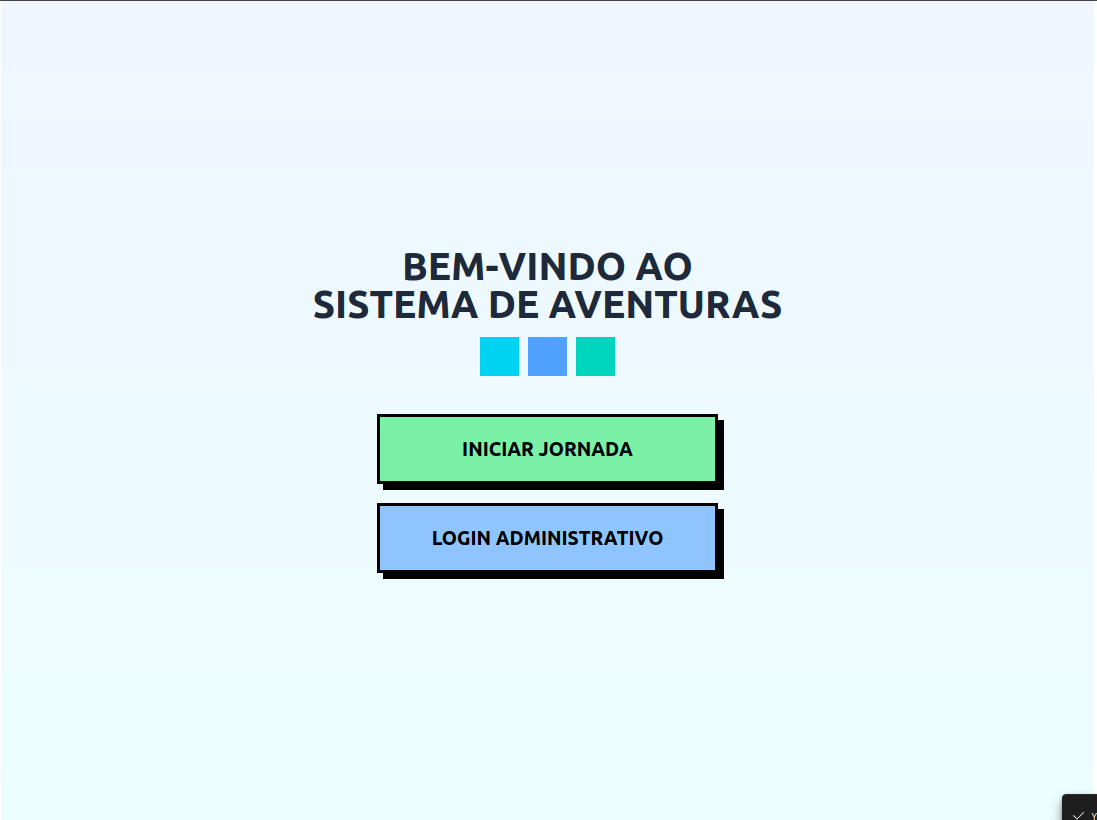
\includegraphics[width=0.85\textwidth]{tela01_home.png}
  \caption*{\small\textit{Fonte: Autoria própria, 2026.}}
\end{figure}
\textbf{Tela Inicial (Home):} Atua como o ponto de entrada principal (\textit{Boundary}) do
sistema, apresentando uma interface minimalista com identidade visual lúdica e alto
contraste para facilitar a navegação. O projeto foca no controle de acesso através de dois
caminhos distintos: o início da jornada para o usuário final e o login administrativo para
gestores, permitindo a separação de responsabilidades entre os perfis de usuário logo na
primeira interação.
 
\begin{figure}[H]
  \centering
  \caption*{Figura 2: Acesso do Explorador (Autenticação).}
  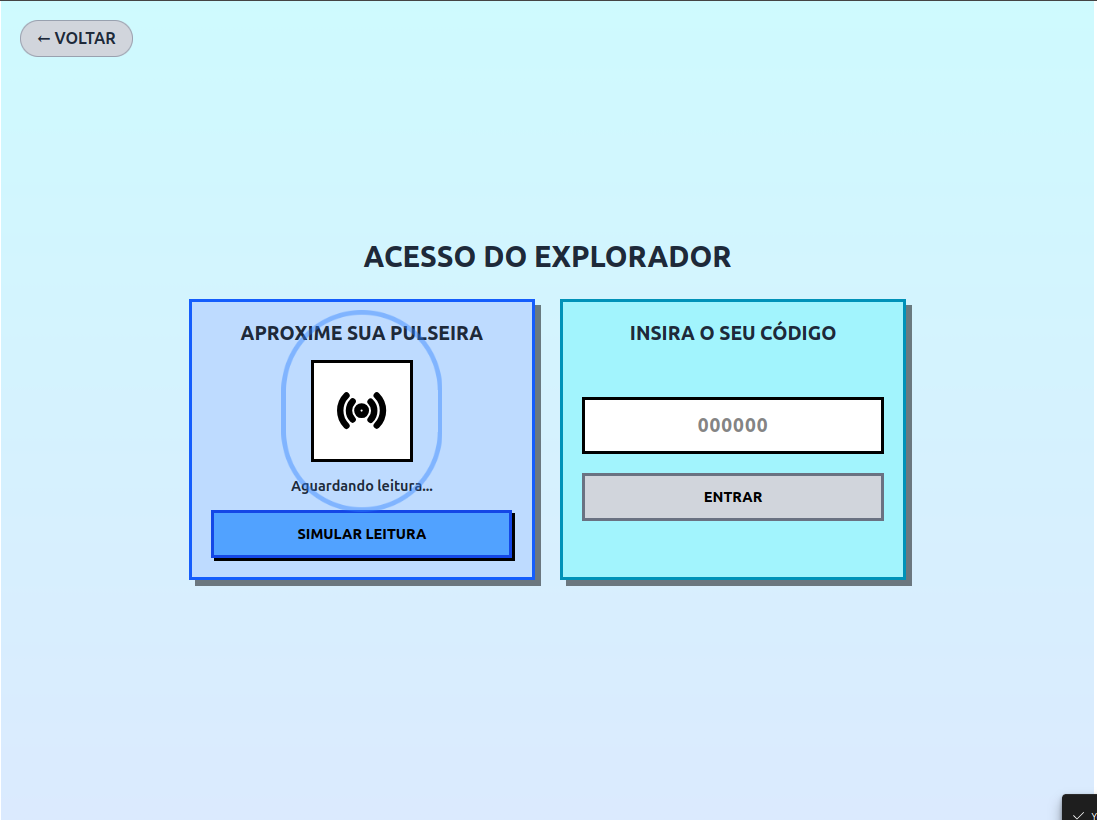
\includegraphics[width=0.85\textwidth]{tela02_acesso.png}
  \caption*{\small\textit{Fonte: Autoria própria, 2026.}}
\end{figure}
\textbf{Acesso do Explorador (Autenticação):} Esta interface implementa a lógica de
autenticação do objeto \texttt{Explorador}, oferecendo métodos de entrada por hardware
(simulação de leitura de pulseira via sensor) ou por entrada manual de código numérico. O
design prioriza a autonomia do usuário com deficiência intelectual, utilizando ícones
autoexplicativos e botões de comando claros para reduzir a carga cognitiva durante o
processo de identificação no sistema.
 
\begin{figure}[H]
  \centering
  \caption*{Figura 3: Mural do Explorador (Dashboard).}
  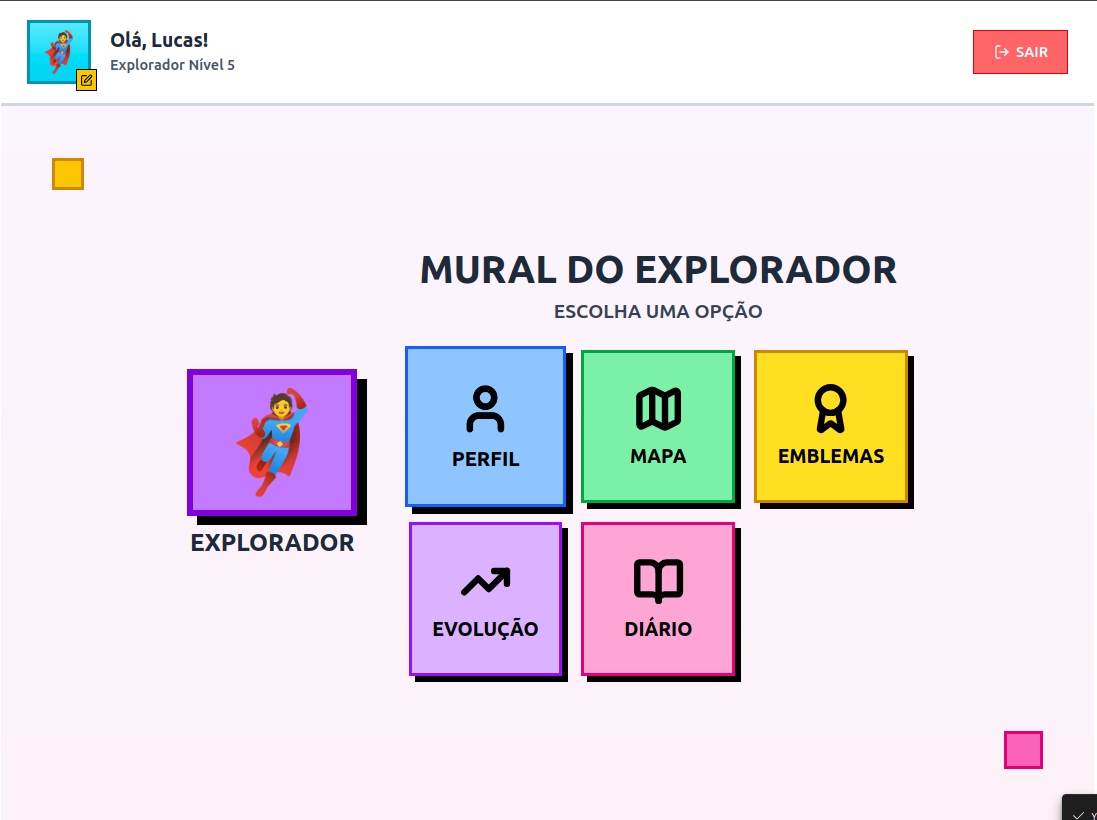
\includegraphics[width=0.85\textwidth]{tela03_mural.png}
  \caption*{\small\textit{Fonte: Autoria própria, 2026.}}
\end{figure}
\textbf{Mural do Explorador (Dashboard):} Funciona como o hub central de navegação,
onde o usuário visualiza seu estado atual (nível e avatar) e acessa os principais módulos do
sistema por meio de uma grade de objetos interativos. A tela organiza as funcionalidades de
Perfil, Mapa, Emblemas, Evolução e Diário em blocos coloridos e distintos, servindo como
uma fachada (\textit{Facade}) para as diversas áreas de interesse do aluno dentro da
aplicação.
 
\begin{figure}[H]
  \centering
  \caption*{Figura 4: Editar Avatar (Customização).}
  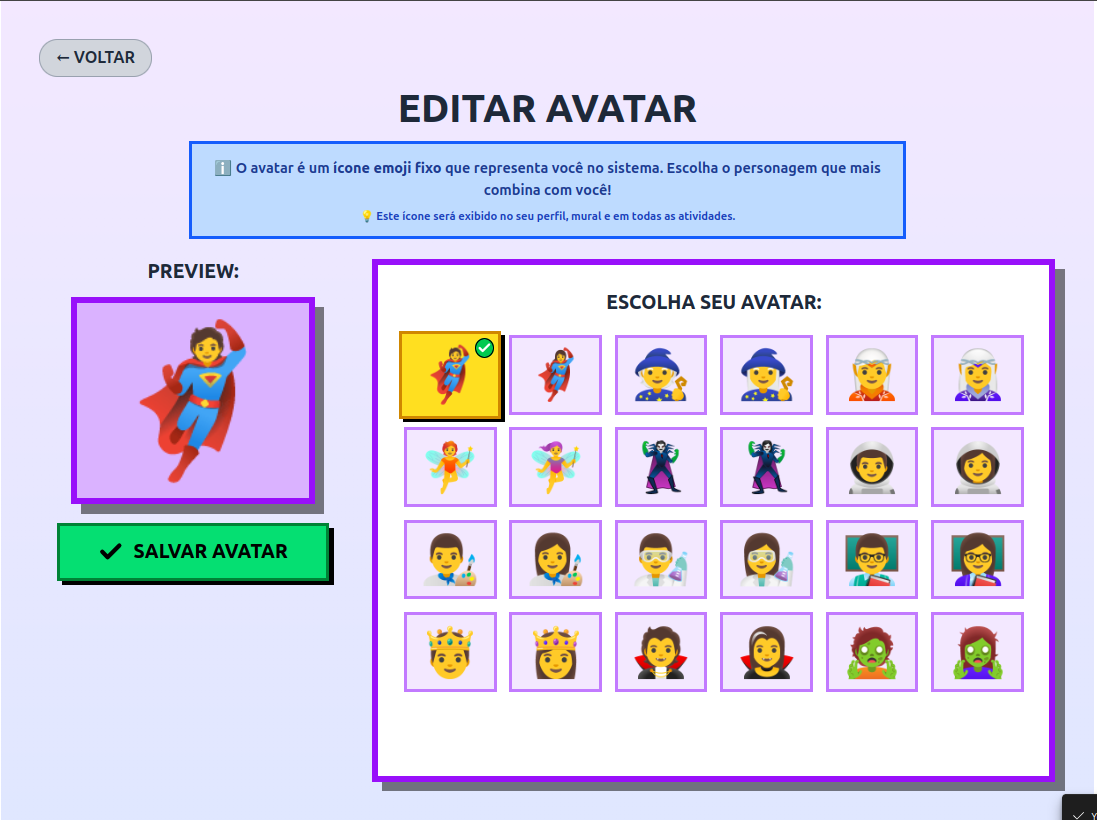
\includegraphics[width=0.85\textwidth]{tela04_avatar.png}
  \caption*{\small\textit{Fonte: Autoria própria, 2026.}}
\end{figure}
\textbf{Editar Avatar (Customização):} Esta tela permite a manipulação dos atributos
estéticos do objeto \texttt{Explorador}, oferecendo uma galeria de opções visuais para
personalização da identidade digital. A interface inclui uma área de visualização prévia
(\textit{Preview}) que responde em tempo real à seleção do usuário, garantindo que a
alteração seja confirmada apenas após a interação com o comando de persistência de dados.
 
\begin{figure}[H]
  \centering
  \caption*{Figura 5: Perfil do Herói --- Dados e Estatísticas (parte superior e inferior).}
  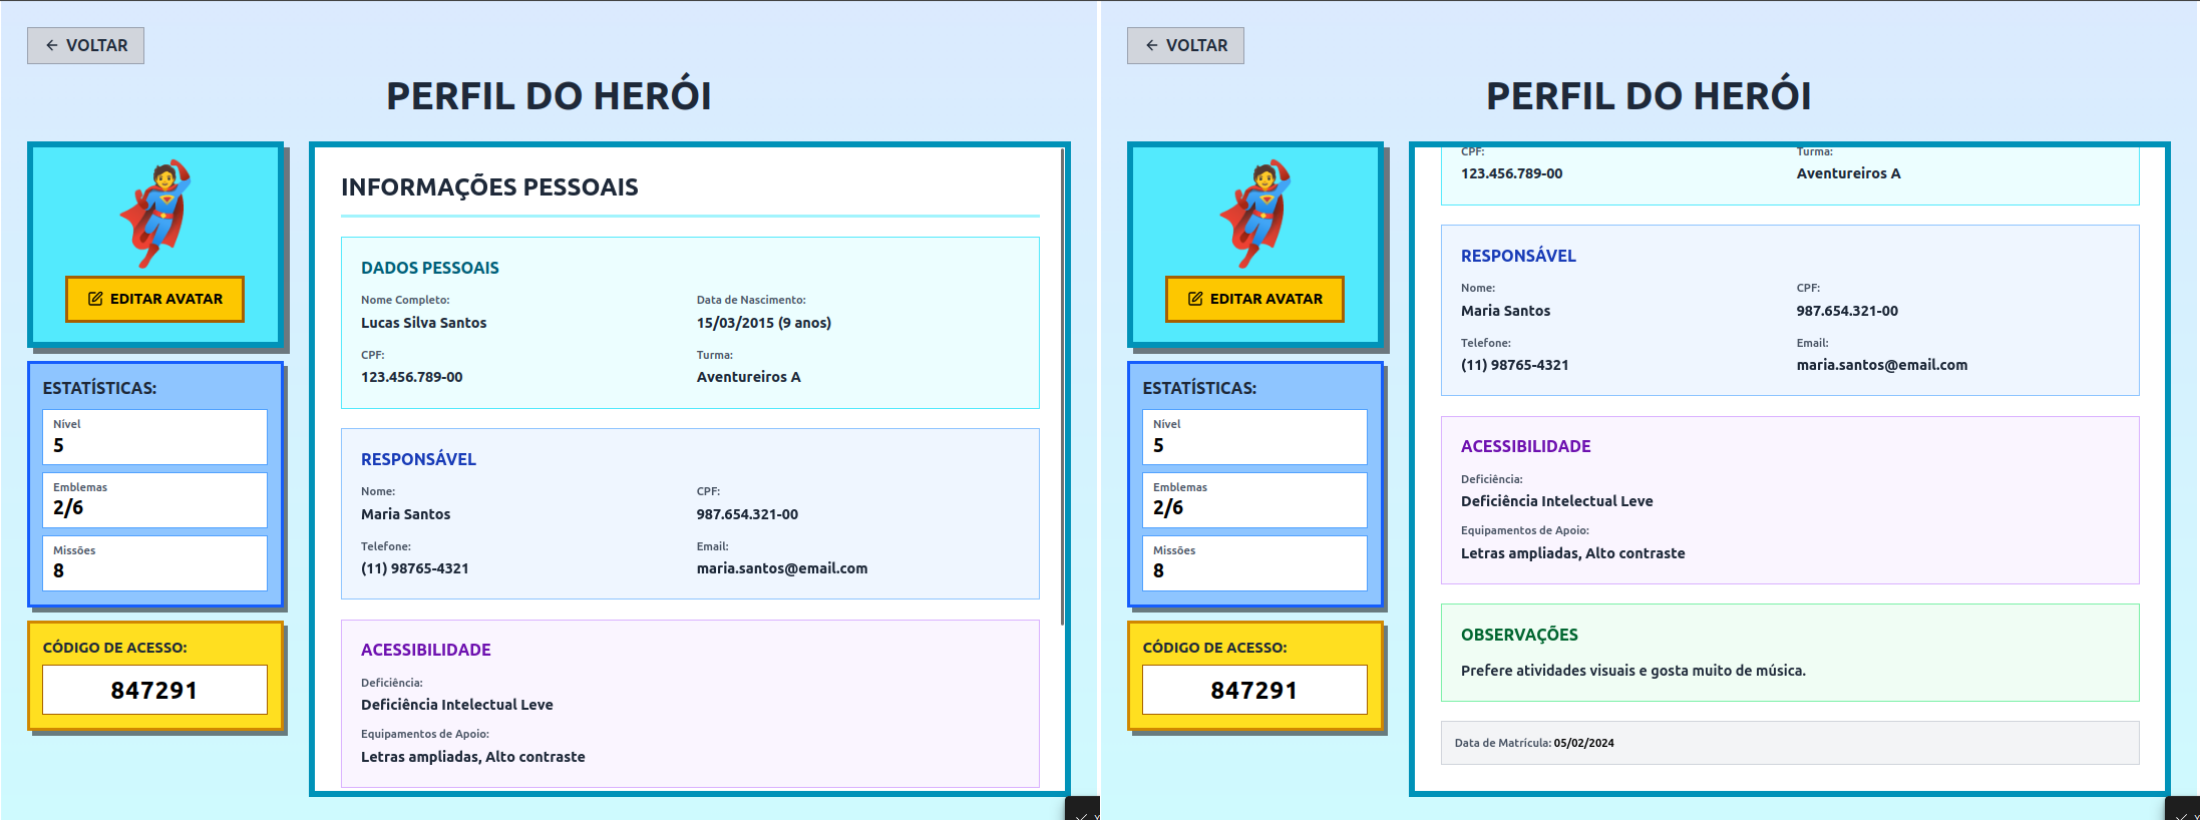
\includegraphics[width=0.85\textwidth]{tela05_perfil1.png}
  \caption*{\small\textit{Fonte: Autoria própria, 2026.}}
\end{figure}
\textbf{Perfil do Herói (Dados e Estatísticas):} Apresenta uma visão detalhada dos
atributos da classe \texttt{Explorador} e suas associações com as classes
\texttt{Responsável} e \texttt{Acessibilidade}, organizando informações cadastrais e de
desempenho. A tela é estruturada em seções lógicas que facilitam a leitura rápida de dados
como nível, missões concluídas, contatos de emergência e as configurações específicas de
acessibilidade necessárias para o suporte ao aluno.
 
\begin{figure}[H]
  \centering
  \caption*{Figura 6: Mapa do Tesouro (Trilha de Aprendizagem).}
  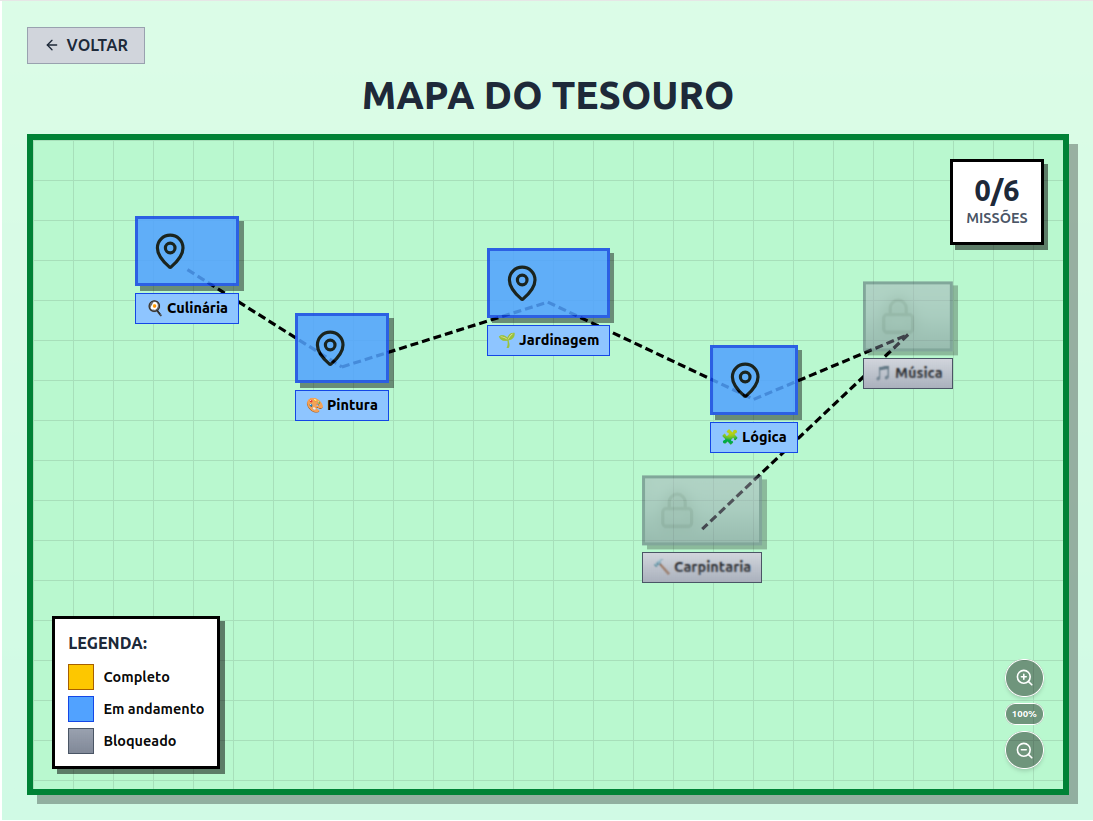
\includegraphics[width=0.85\textwidth]{tela07_mapa.png}
  \caption*{\small\textit{Fonte: Autoria própria, 2026.}}
\end{figure}
\textbf{Mapa do Tesouro (Trilha de Aprendizagem):} Representa graficamente o progresso
pedagógico através de uma estrutura de grafos, onde cada nó corresponde a uma instância
da classe \texttt{Missão}. A interface utiliza uma legenda de estados (Completo, Em
Andamento e Bloqueado) para gerenciar o fluxo de navegação do aluno, garantindo que a
lógica de pré-requisitos entre as atividades seja respeitada visualmente e sistemicamente.
 
\begin{figure}[H]
  \centering
  \caption*{Figura 7: Missão Culinária --- Salada de Frutas (Execução e Resultado).}
  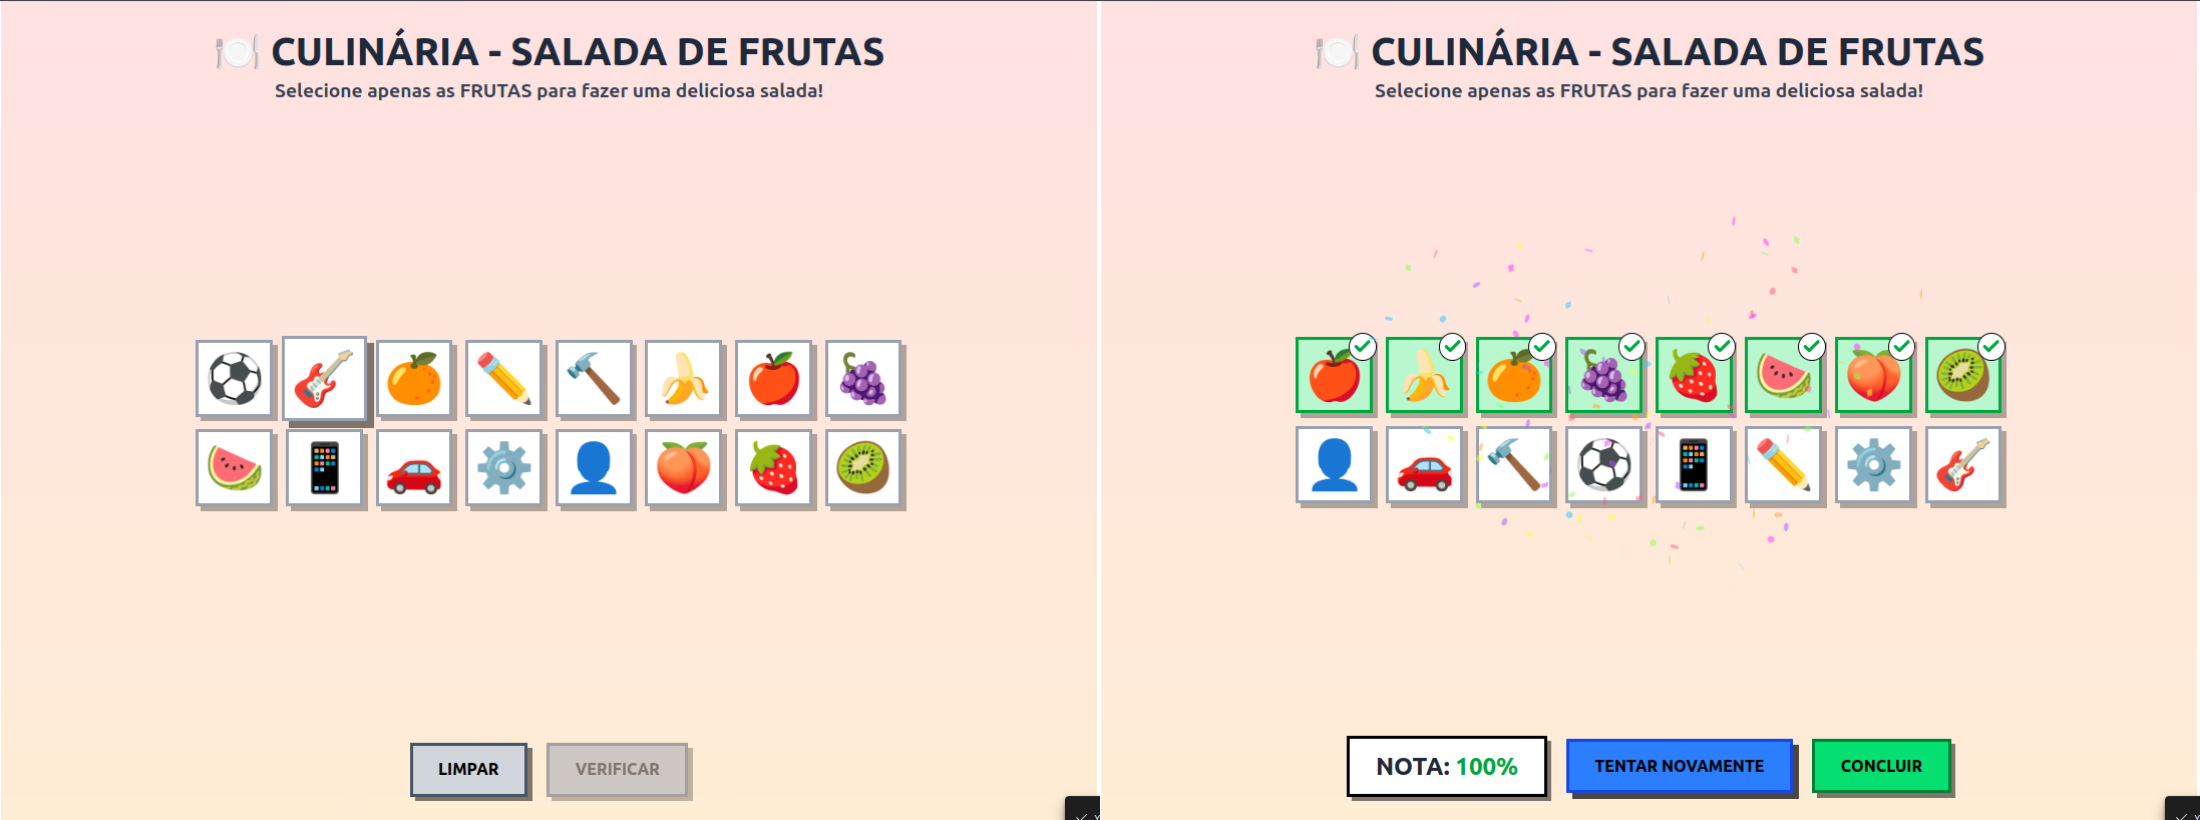
\includegraphics[width=0.85\textwidth]{tela08_culinaria_exec.png}
  \caption*{\small\textit{Fonte: Autoria própria, 2026.}}
\end{figure}
\textbf{Missão Culinária --- Salada de Frutas (Execução):} Interface de atividade
pedagógica que implementa a lógica de classificação de objetos, onde o usuário deve
interagir com uma coleção de itens para identificar elementos pertencentes à categoria
``Frutas''. A tela conta com métodos de controle para limpar a seleção atual ou submeter as
respostas para validação, testando as habilidades de discriminação visual e lógica do
explorador.
 
\textbf{Missão Culinária (Feedback de Resultado):} Tela de retorno que processa e exibe
o resultado da atividade anterior, utilizando reforços positivos visuais e métricas de
desempenho (nota percentual). Esta interface permite ao usuário decidir entre a repetição da
tarefa para melhoria de desempenho ou a conclusão definitiva, o que desencadeia a
atualização do estado da missão no objeto de progresso do aluno.
 
\begin{figure}[H]
  \centering
  \caption*{Figura 8: Missão Pintura --- Pinte o Desenho (Atividade Criativa e Finalizada).}
  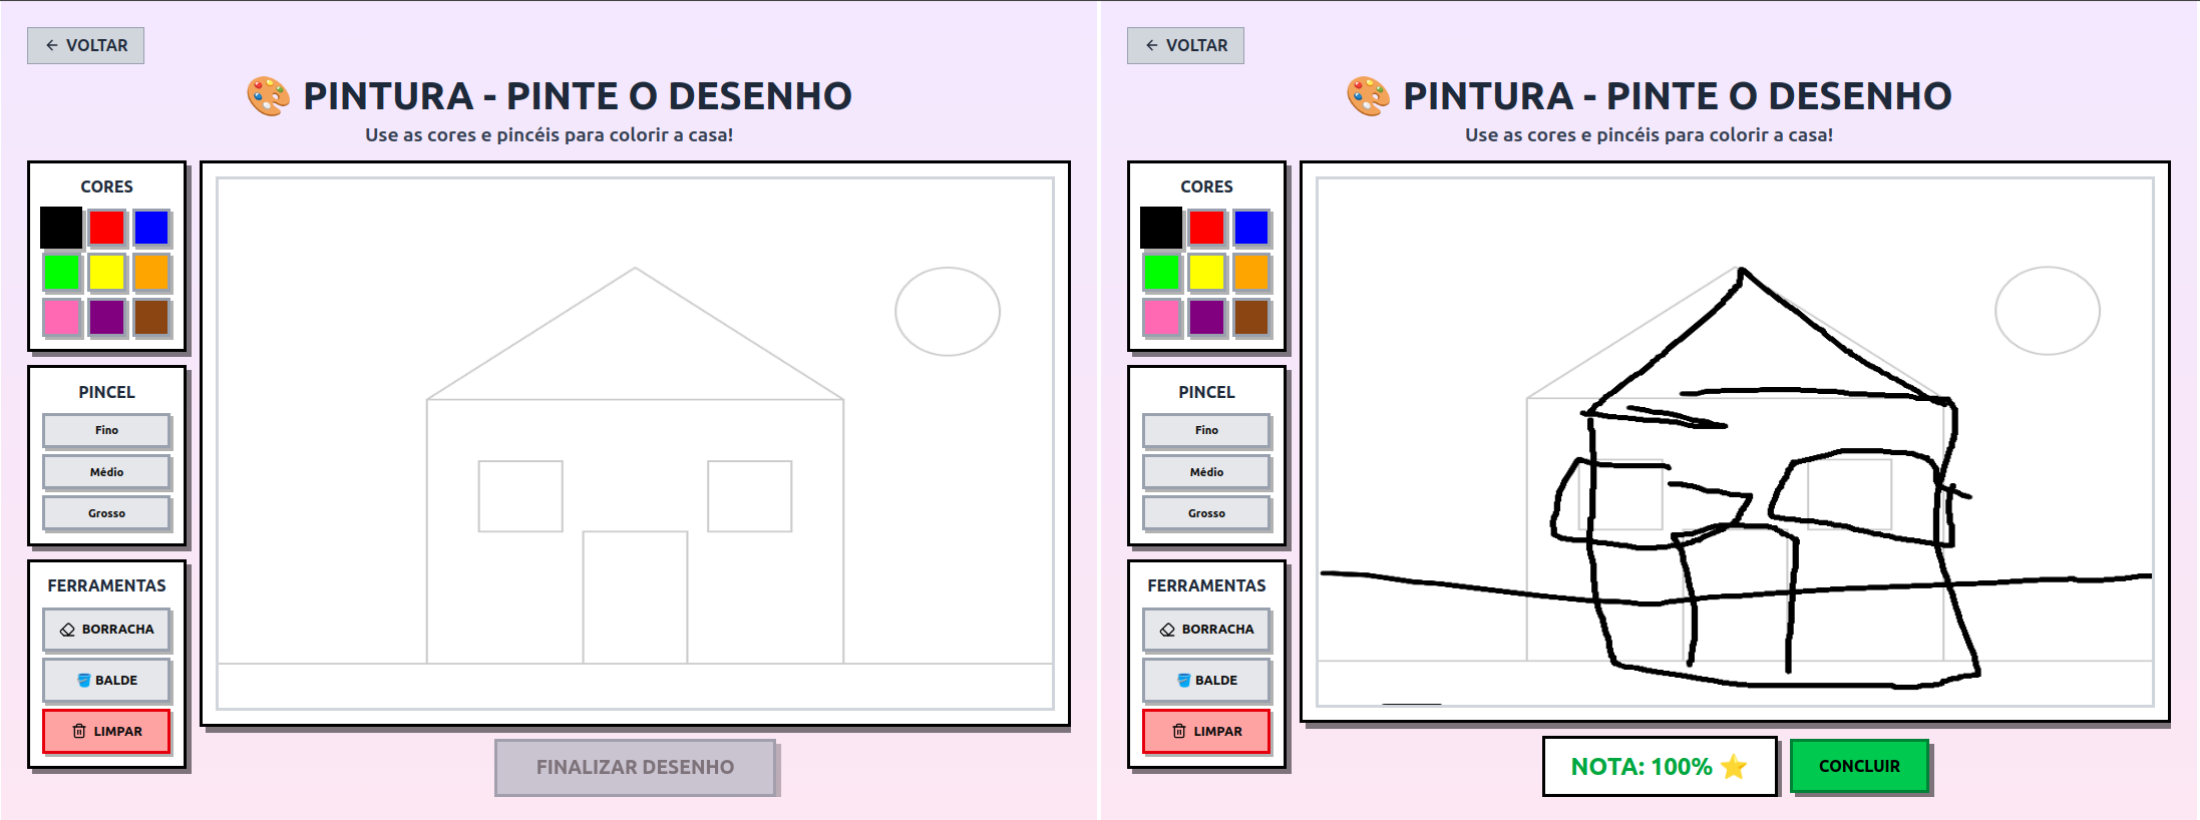
\includegraphics[width=0.85\textwidth]{tela10_pintura_exec.png}
  \caption*{\small\textit{Fonte: Autoria própria, 2026.}}
\end{figure}
\textbf{Missão Pintura (Atividade Criativa):} Interface de interação livre que disponibiliza
ferramentas para manipulação de cores e pincéis sobre um modelo pré-definido, visando o
desenvolvimento da motricidade fina. O projeto desta tela inclui um conjunto de comandos
para gestão do \textit{canvas} (limpar, balde de tinta, borracha), transformando a entrada
do usuário em dados visuais persistentes dentro do ambiente de aprendizagem.
 
\textbf{Missão Pintura --- Finalizada:} Esta interface de encerramento de atividade processa
os dados gerados no \textit{canvas} e apresenta o resultado final ao usuário, integrando
mecanismos de \textit{feedback} imediato que validam a conclusão da tarefa com uma nota
de aproveitamento. O objeto de controle gerencia a transição de estado da atividade,
permitindo que o explorador avance na jornada pedagógica ou retorne ao mapa principal.
 
\begin{figure}[H]
  \centering
  \caption*{Figura 9: Missão Jardinagem --- Plantar e Regar (Execução e Resultado).}
  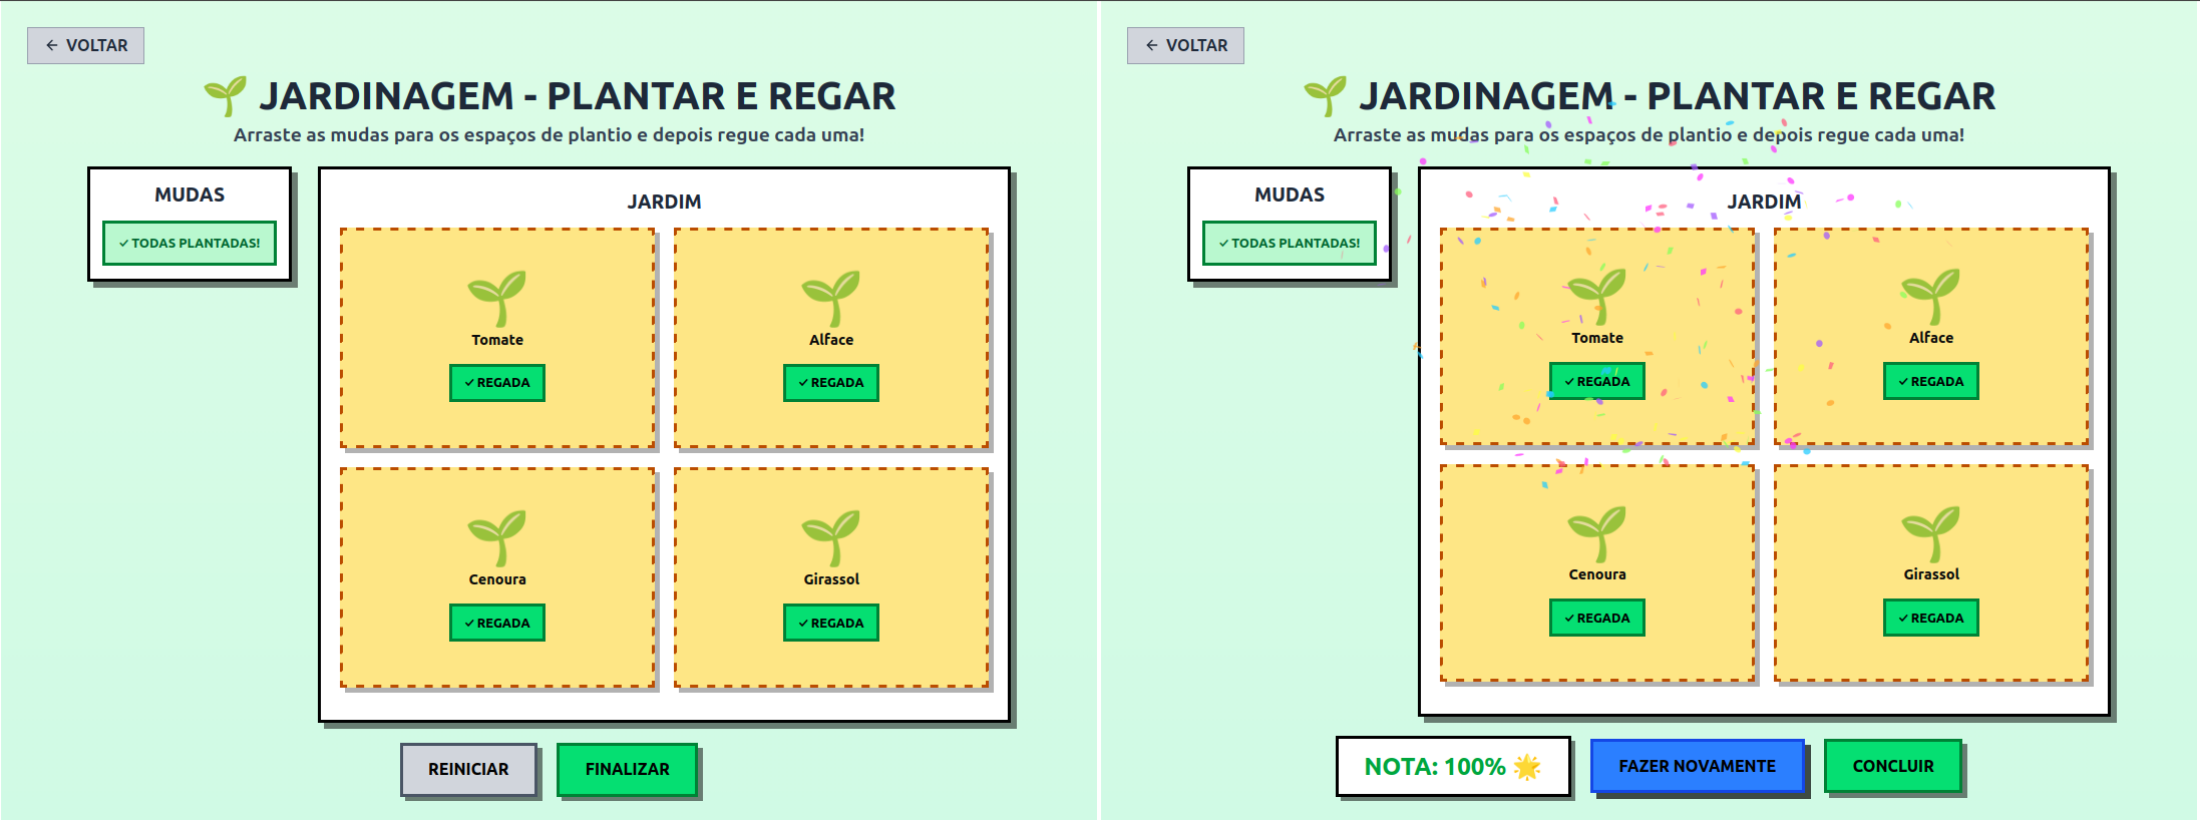
\includegraphics[width=0.85\textwidth]{tela12_jardinagem_exec.png}
  \caption*{\small\textit{Fonte: Autoria própria, 2026.}}
\end{figure}
\textbf{Missão Jardinagem (Execução):} Esta tela implementa uma lógica de interação
baseada em eventos de ``arrastar e soltar'' (\textit{Drag and Drop}), onde o usuário deve
associar mudas de plantas aos seus respectivos espaços de cultivo e, sequencialmente,
acionar o método de regar. A interface utiliza estados visuais claros (como o selo
``Regada'') para indicar a conclusão de sub-etapas da tarefa, auxiliando na compreensão de
sequenciamento lógico e cuidado procedimental.
 
\textbf{Missão Jardinagem (Resultado):} Funciona como a tela de encerramento do módulo
de jardinagem, exibindo o status final das plantas cultivadas e a pontuação obtida pelo
explorador através de um componente de progresso percentual. A interface utiliza elementos
festivos (confetes) como reforço positivo e oferece opções de fluxo para repetir a instância
da atividade ou consolidar o progresso no perfil do usuário.
 
\begin{figure}[H]
  \centering
  \caption*{Figura 10: Missão Quebra-Cabeça (Execução e Resultado).}
  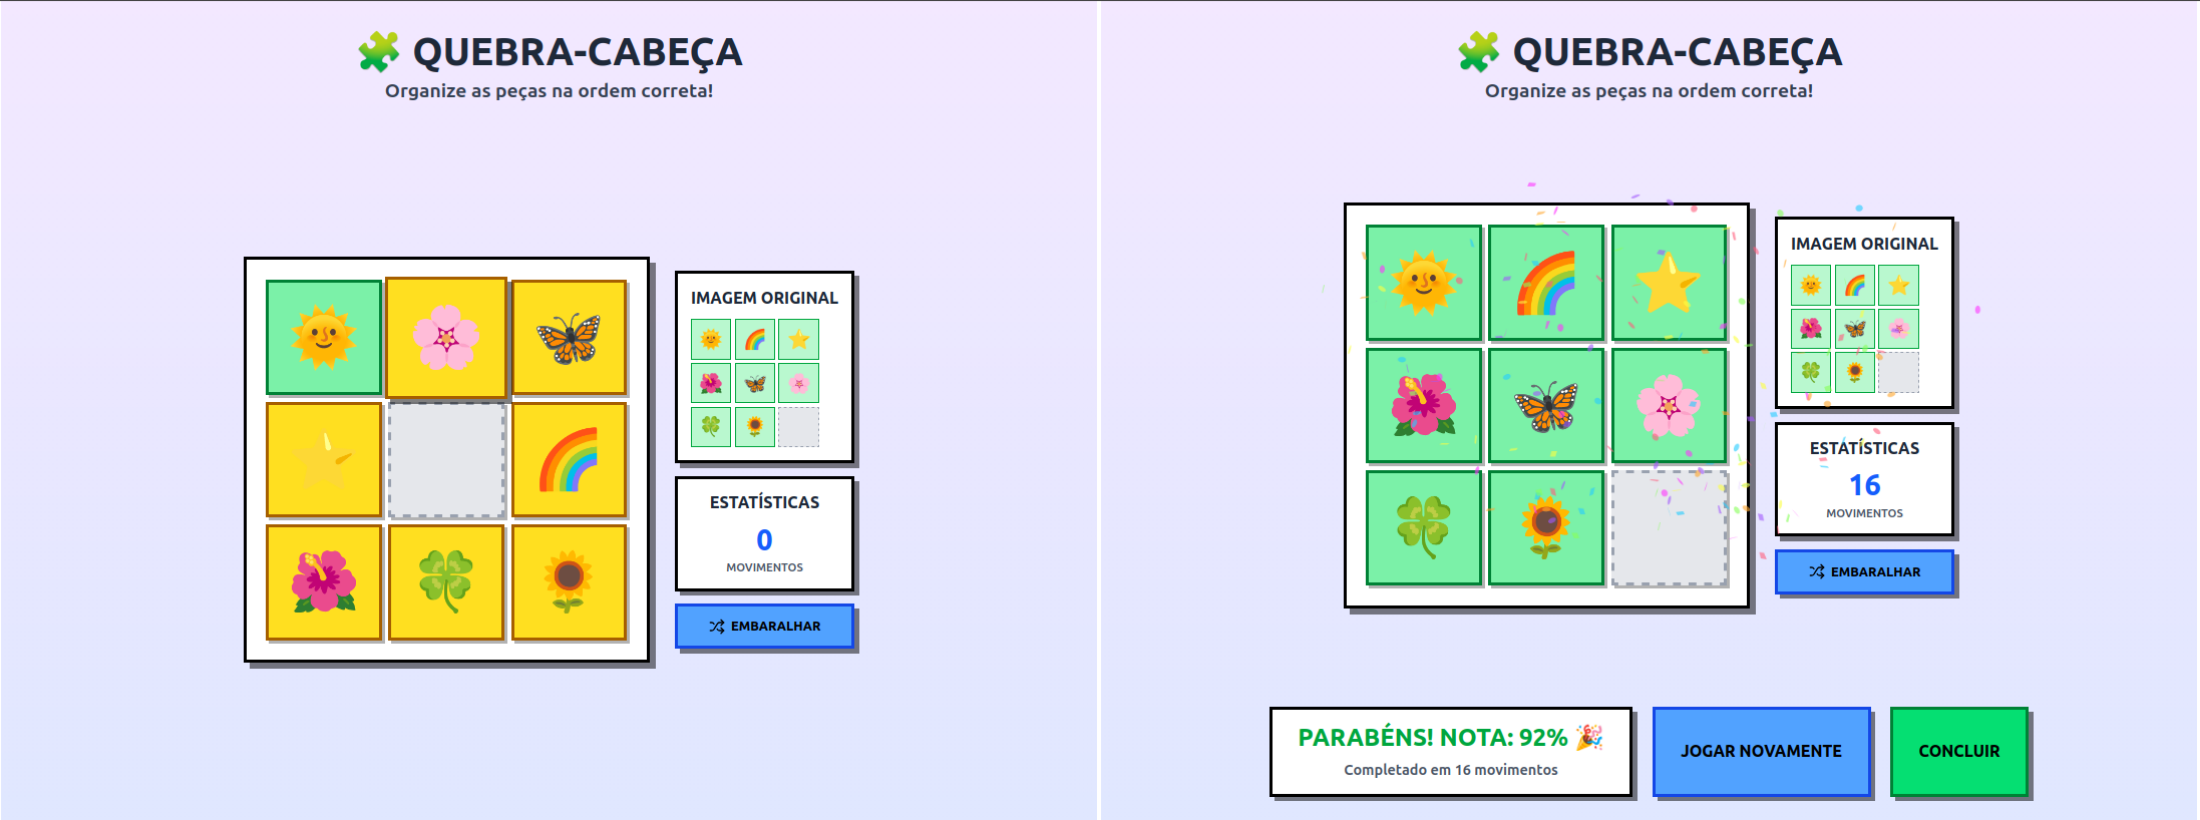
\includegraphics[width=0.85\textwidth]{tela14_quebracabeca_exec.png}
  \caption*{\small\textit{Fonte: Autoria própria, 2026.}}
\end{figure}
\textbf{Missão Quebra-Cabeça (Execução):} Esta interface apresenta um desafio de
organização espacial que manipula um \textit{array} de imagens fragmentadas, exigindo que
o usuário ordene as peças conforme um modelo de referência (objeto original). O sistema
monitora dinamicamente o atributo de ``movimentos'' e oferece um método de embaralhamento
para reiniciar o estado do jogo, estimulando funções executivas e percepção visual.
 
\textbf{Missão Quebra-Cabeça (Resultado):} Apresenta o fechamento da atividade de
raciocínio lógico, exibindo o desempenho final baseado no número de movimentos utilizados
e no percentual de montagem correta. A tela atua como um validador de conclusão para o
objeto \texttt{Missao}, atualizando os registros de conquistas do aluno e permitindo a
progressão para novos desafios dentro da arquitetura do mapa de aprendizagem.
 
\begin{figure}[H]
  \centering
  \caption*{Figura 11: Coleção de Emblemas.}
  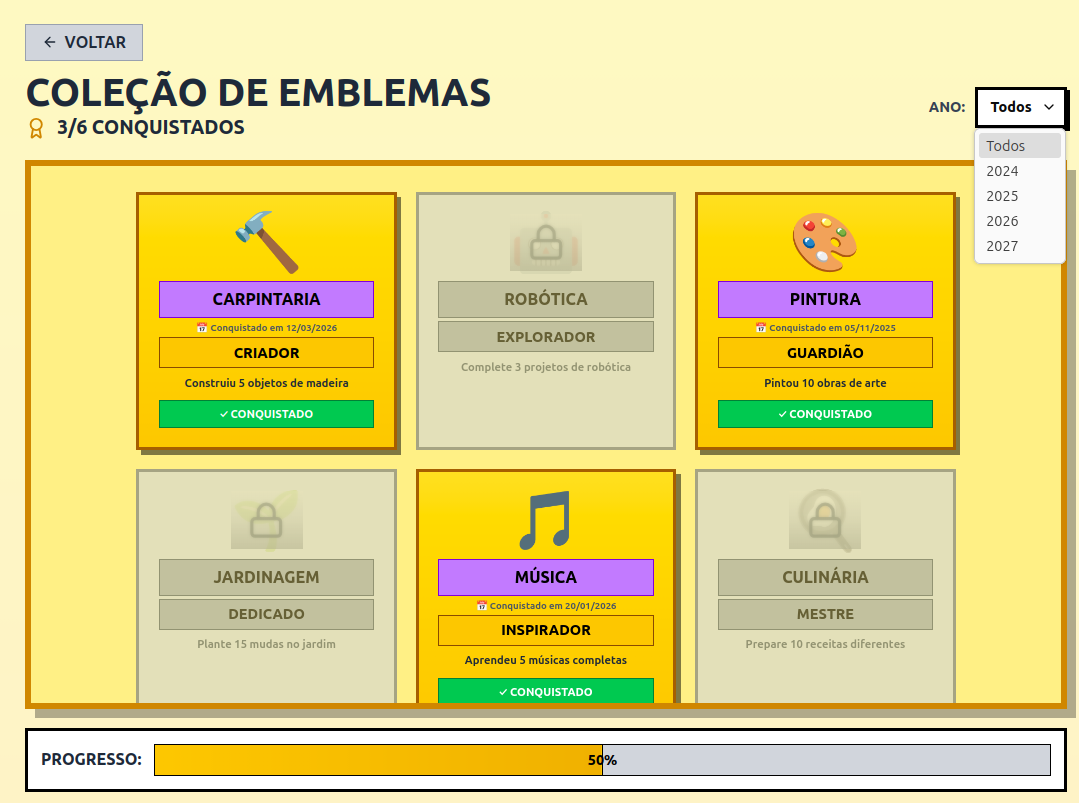
\includegraphics[width=0.85\textwidth]{tela16_emblemas.png}
  \caption*{\small\textit{Fonte: Autoria própria, 2026.}}
\end{figure}
\textbf{Coleção de Emblemas:} Esta tela atua como um repositório visual (\textit{Gallery})
que exibe as instâncias da classe \texttt{Emblema} conquistadas pelo explorador,
diferenciando conquistas ativas de bloqueadas através de filtros de saturação e opacidade.
A interface fornece uma visão consolidada do progresso geral do usuário por meio de uma
barra de progresso totalizadora, incentivando a completitude das atividades pedagógicas
distribuídas por categorias.
 
\begin{figure}[H]
  \centering
  \caption*{Figura 12: Evolução do Poder (Dashboard de Progressão).}
  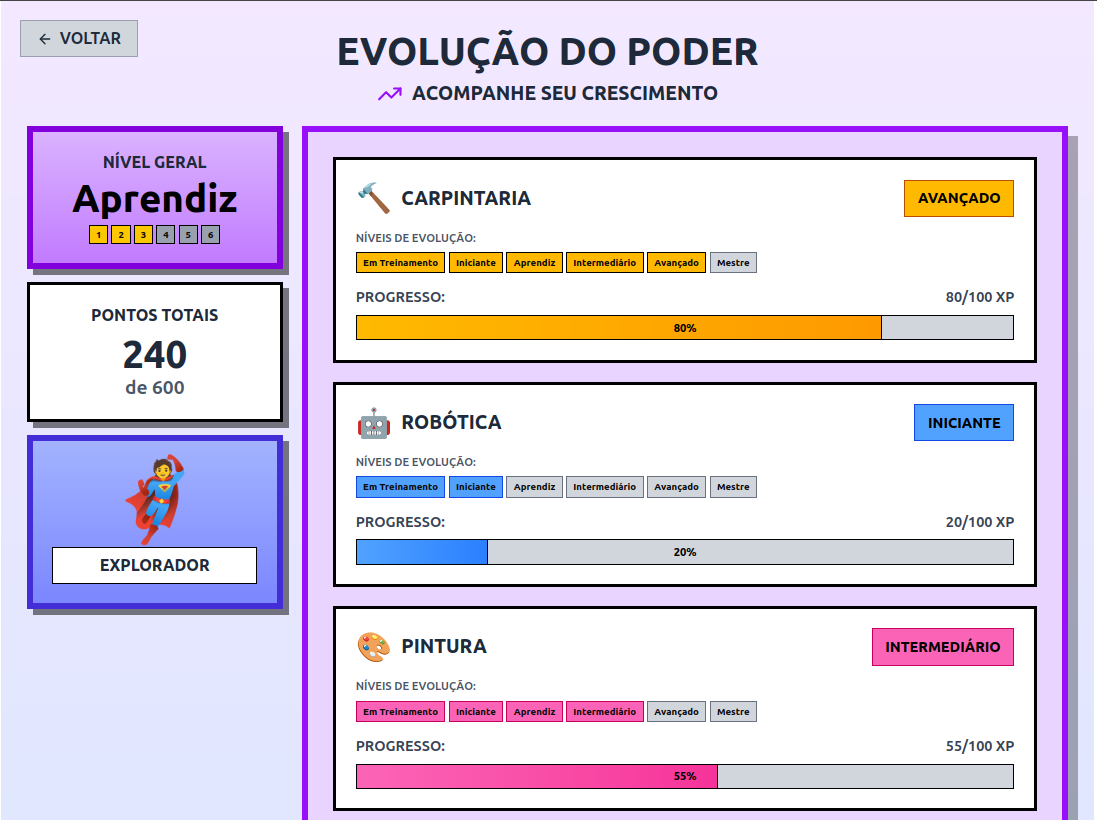
\includegraphics[width=0.85\textwidth]{tela17_evolucao.png}
  \caption*{\small\textit{Fonte: Autoria própria, 2026.}}
\end{figure}
\textbf{Evolução do Poder (Dashboard de Progressão):} Esta interface detalha o nível de
proficiência do usuário em diferentes competências (Carpintaria, Robótica, Pintura),
mapeando o progresso acumulado em barras de experiência (XP) específicas por categoria.
O design organiza os dados de forma que o aluno possa visualizar seu crescimento individual
em cada ``árvore de habilidades'', traduzindo métricas técnicas em nomenclaturas lúdicas
como ``Aprendiz'', ``Intermediário'' e ``Avançado''.
 
\begin{figure}[H]
  \centering
  \caption*{Figura 13: Diário do Explorador (Logs de Atividade).}
  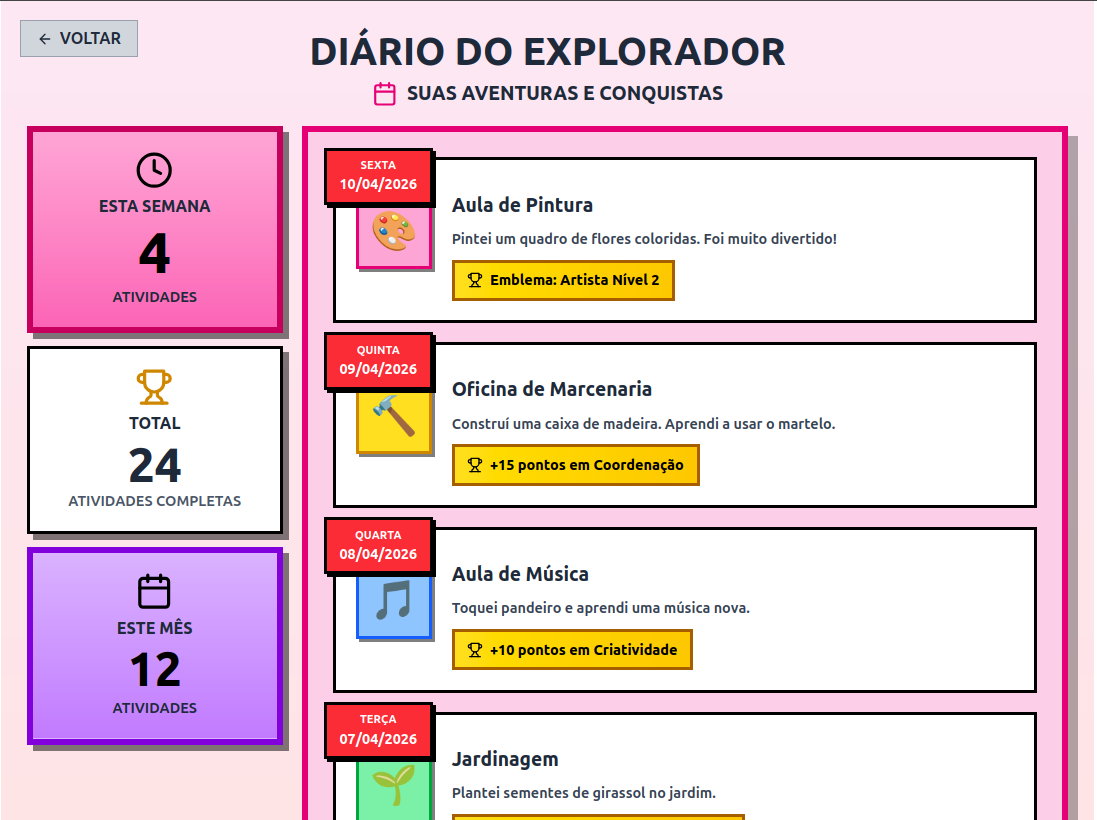
\includegraphics[width=0.85\textwidth]{tela18_diario.png}
  \caption*{\small\textit{Fonte: Autoria própria, 2026.}}
\end{figure}
\textbf{Diário do Explorador (Logs de Atividade):} Funciona como um histórico
cronológico de interações, listando as atividades concluídas e as recompensas obtidas em
cada data específica dentro da aplicação. Esta tela organiza os objetos de \textit{log} de
forma a fornecer estatísticas temporais (semanais e mensais) para o aluno e seus
responsáveis, facilitando o acompanhamento do engajamento e da evolução contínua dentro
do sistema.
 
% ==============================================================
\subsection{INTERFACES DO PERFIL ADMINISTRATIVO}
% ==============================================================
 
% --------------------------------------------------------------
\subsubsection{Mestre da Jornada}
% --------------------------------------------------------------
 
\begin{figure}[H]
  \centering
  \caption*{Figura 14: Login Administrativo --- Seleção de Perfil.}
  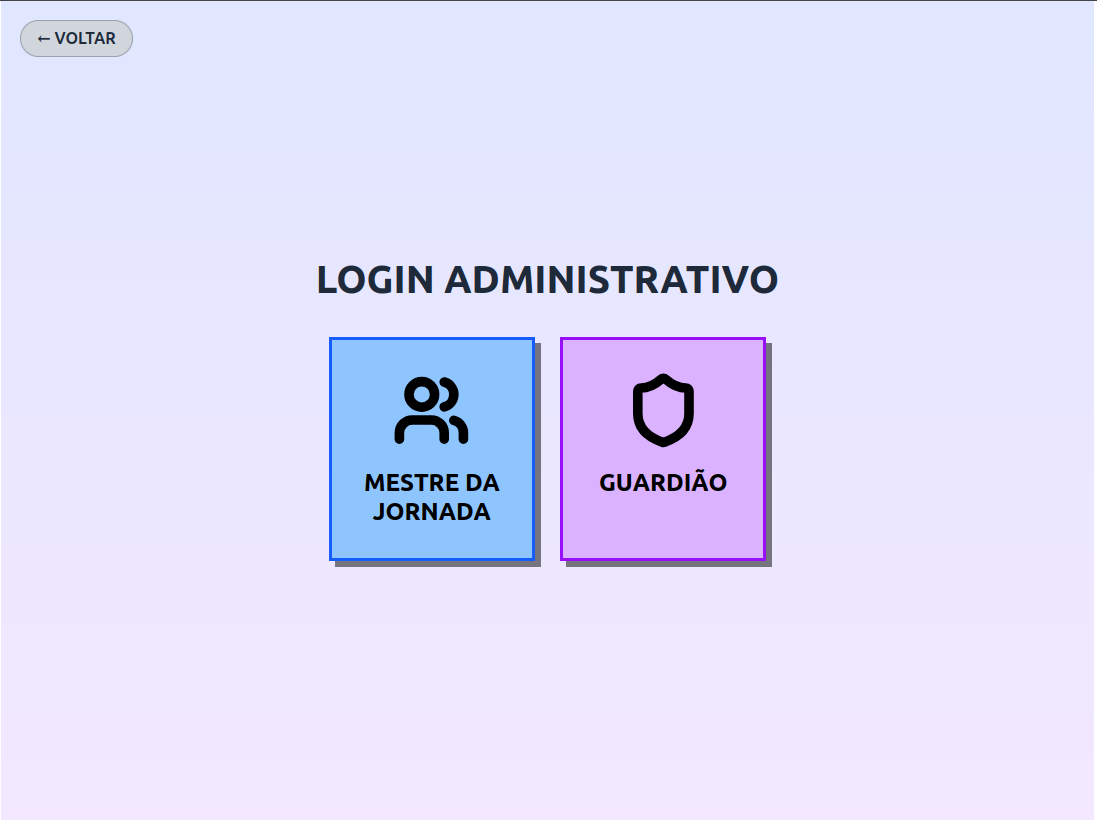
\includegraphics[width=0.85\textwidth]{adm01_login_selecao.png}
  \caption*{\small\textit{Fonte: Autoria própria, 2026.}}
\end{figure}
\textbf{Login Administrativo --- Seleção de Perfil:} Esta interface de fronteira
(\textit{Boundary}) direciona o acesso administrativo, permitindo ao usuário escolher entre
os papéis de ``Mestre da Jornada'' (professor) e ``Guardião'' (pedagogo) antes de inserir
suas credenciais. O design separa visualmente os dois perfis em blocos distintos e
iconograficamente diferenciados, garantindo que cada tipo de usuário seja encaminhado ao
seu respectivo ambiente de gestão de forma clara e sem ambiguidade.
 
\begin{figure}[H]
  \centering
  \caption*{Figura 15: Login Administrativo --- Formulário de Acesso (Mestre da Jornada).}
  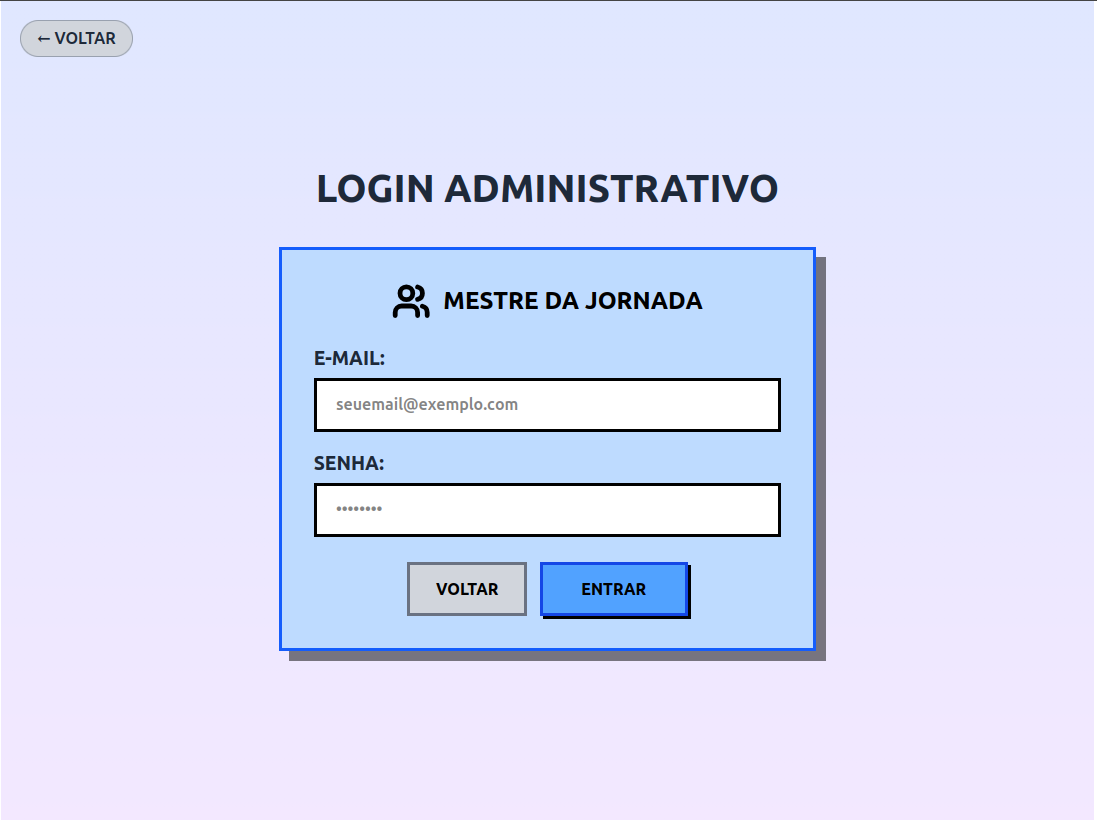
\includegraphics[width=0.85\textwidth]{adm02_login_form.png}
  \caption*{\small\textit{Fonte: Autoria própria, 2026.}}
\end{figure}
\textbf{Login Administrativo --- Formulário de Acesso (Mestre da Jornada):} Após a
seleção do perfil, esta tela exibe o formulário padrão de e-mail e senha para validação de
credenciais via classe \texttt{Autenticador}, servindo como portão de entrada às ferramentas
de gestão pedagógica. O design mantém a identidade visual do perfil selecionado por meio
de cores e ícones consistentes, reforçando ao usuário qual papel está sendo autenticado
antes de confirmar o acesso.
 
\begin{figure}[H]
  \centering
  \caption*{Figura 16: Painel do Mestre da Jornada --- (Dashboard).}
  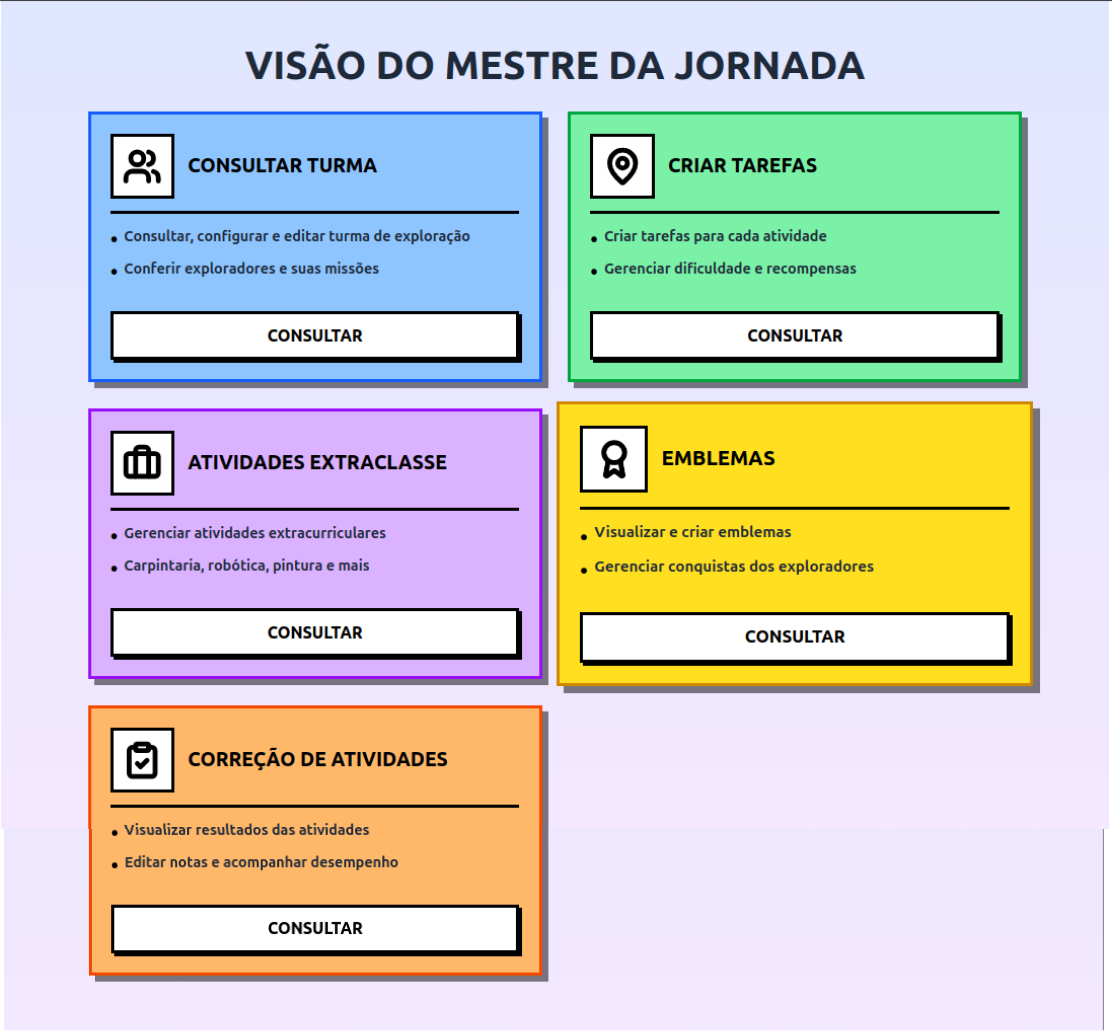
\includegraphics[width=0.85\textwidth]{adm03_painel_mestre.png}
  \caption*{\small\textit{Fonte: Autoria própria, 2026.}}
\end{figure}
\textbf{Painel do Mestre da Jornada (Dashboard):} Atua como o centro de comando do
professor, organizando as funcionalidades de Consultar Turma, Criar Tarefas, Atividades
Extraclasse, Emblemas e Correção de Atividades em cartões coloridos e descritivos. Cada
módulo apresenta um resumo de suas responsabilidades e um botão de acesso direto,
funcionando como uma fachada (\textit{Facade}) que centraliza e distribui as ações
pedagógicas disponíveis ao Mestre da Jornada dentro do ecossistema do sistema.
 
\begin{figure}[H]
  \centering
  \caption*{Figura 17: Visão de Turmas --- Turma ``Aventureiros A'' e Turma ``Aventureiros B''.}
  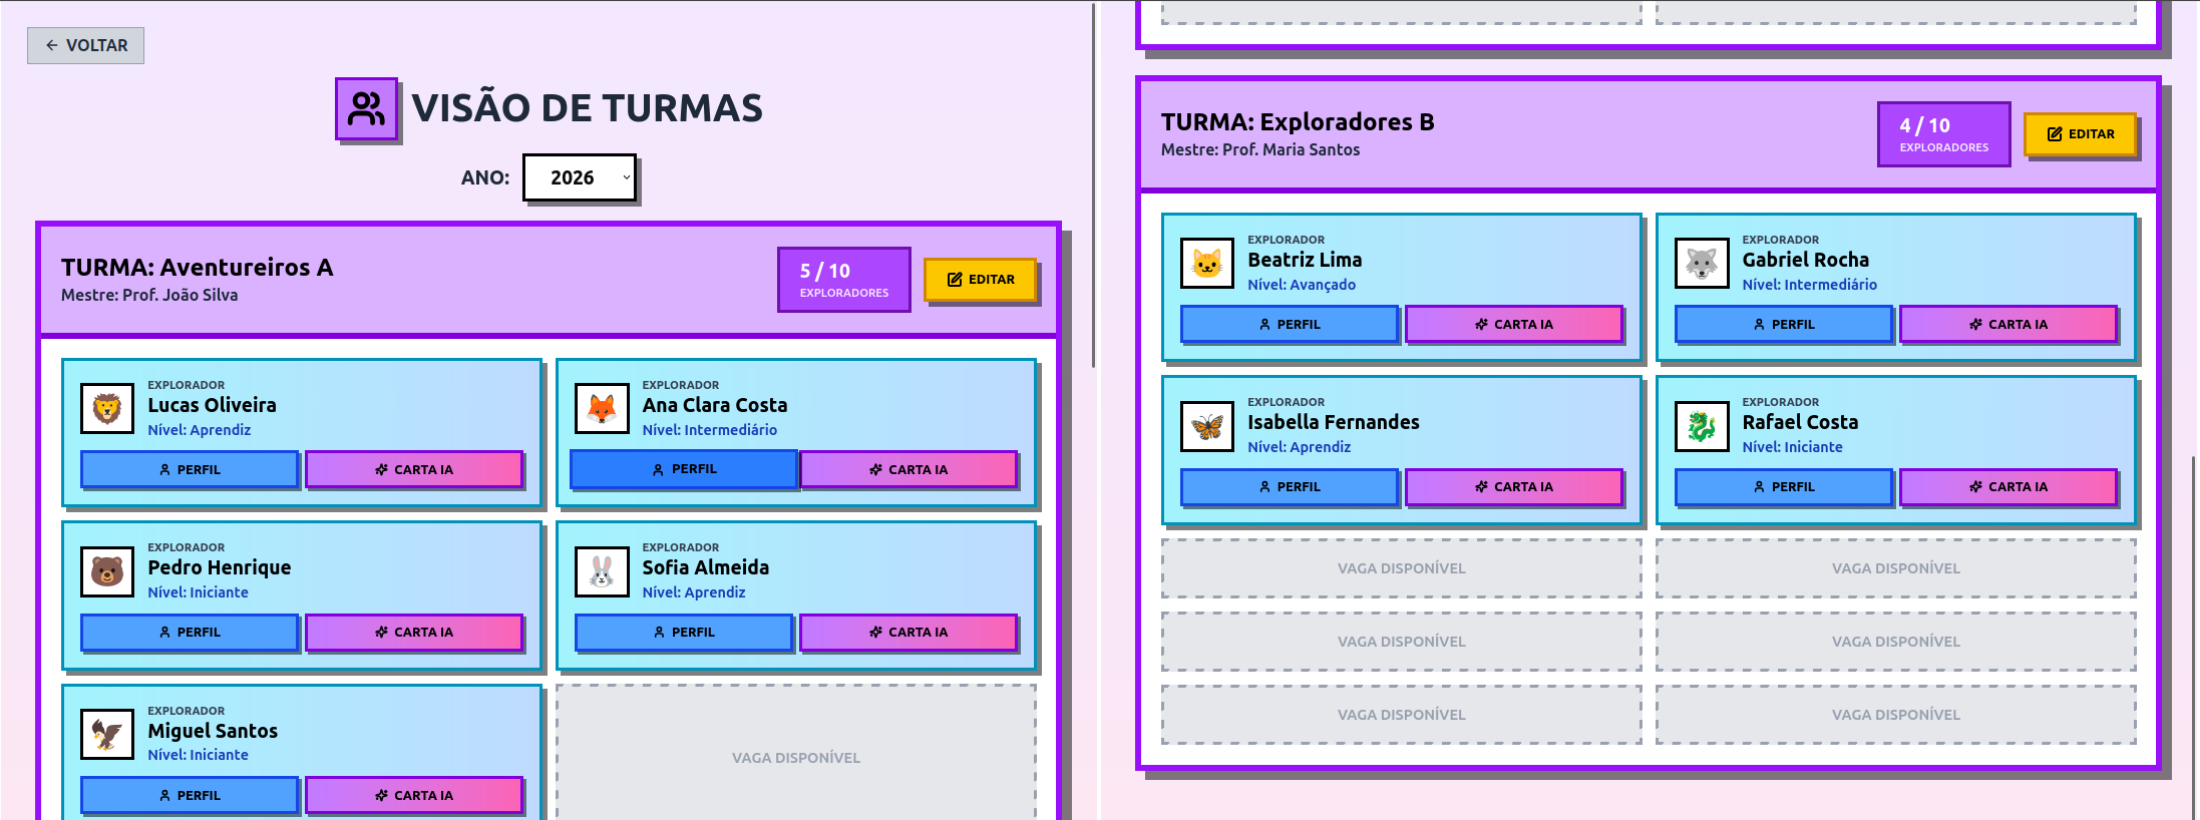
\includegraphics[width=0.85\textwidth]{adm08_visao_turmas2.png}
  \caption*{\small\textit{Fonte: Autoria própria, 2026.}}
\end{figure}
\textbf{Gerenciamento de Turmas --- Visão de Turmas:} Esta tela gerencia as instâncias
da classe \texttt{Turma}, exibindo os cartões de cada \texttt{Explorador} com seu nível
atual e disponibilizando ações diretas de acesso ao perfil individual ou geração de Carta de
Progresso via IA. A interface respeita o limite máximo de dez exploradores por turma,
indicando visualmente as vagas disponíveis, e permite ao professor alternar o ano letivo
para consultar composições históricas das equipes de exploração.
 
\begin{figure}[H]
  \centering
  \caption*{Figura 18: Editar Turma --- Configuração da Equipe de Exploração.}
  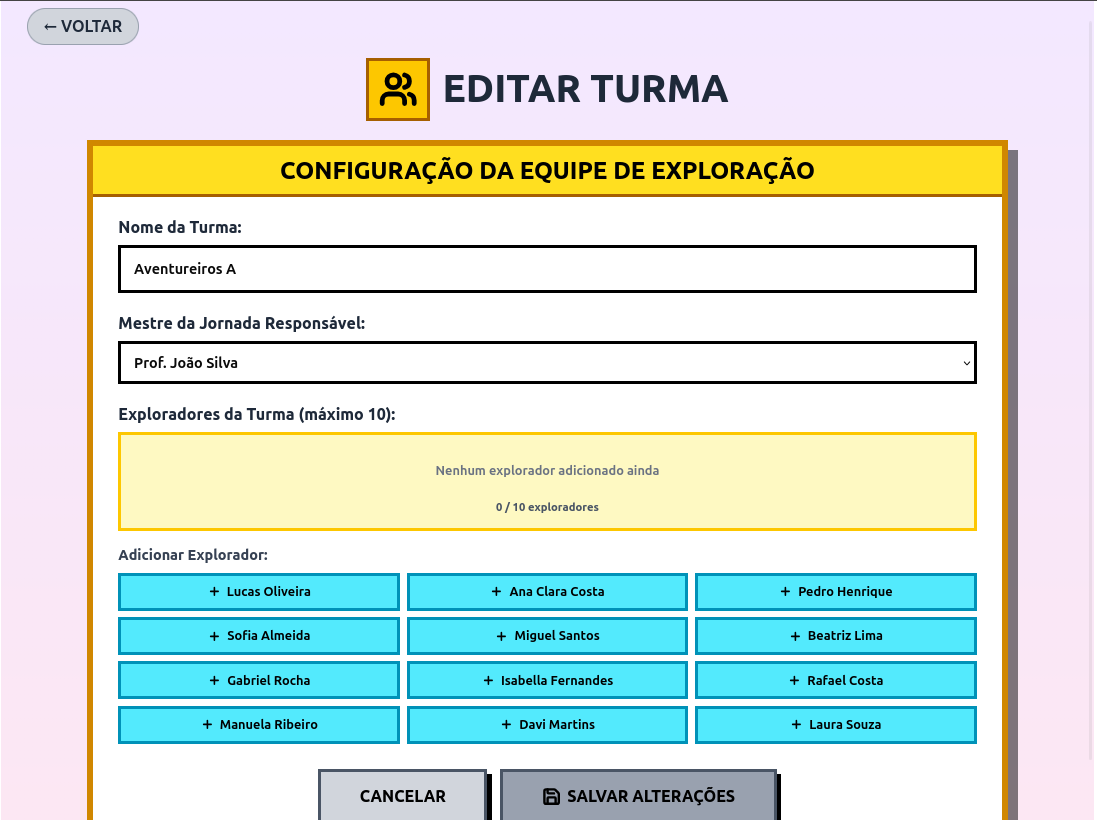
\includegraphics[width=0.85\textwidth]{adm07_editar_turma.png}
  \caption*{\small\textit{Fonte: Autoria própria, 2026.}}
\end{figure}
\textbf{Editar Turma:} Interface de formulário dedicada à gestão dos atributos da classe
\texttt{Turma}, permitindo editar o nome da equipe, vincular um Mestre da Jornada
responsável e adicionar ou remover exploradores do grupo. A tela respeita o limite máximo
de dez exploradores e exibe todos os alunos disponíveis para seleção, garantindo que o
balanceamento pedagógico seja mantido de forma controlada antes de persistir as alterações.
 
\begin{figure}[H]
  \centering
  \caption*{Figura 19: Carta de Progresso IA --- Seleção de Período e Resultado Gerado.}
  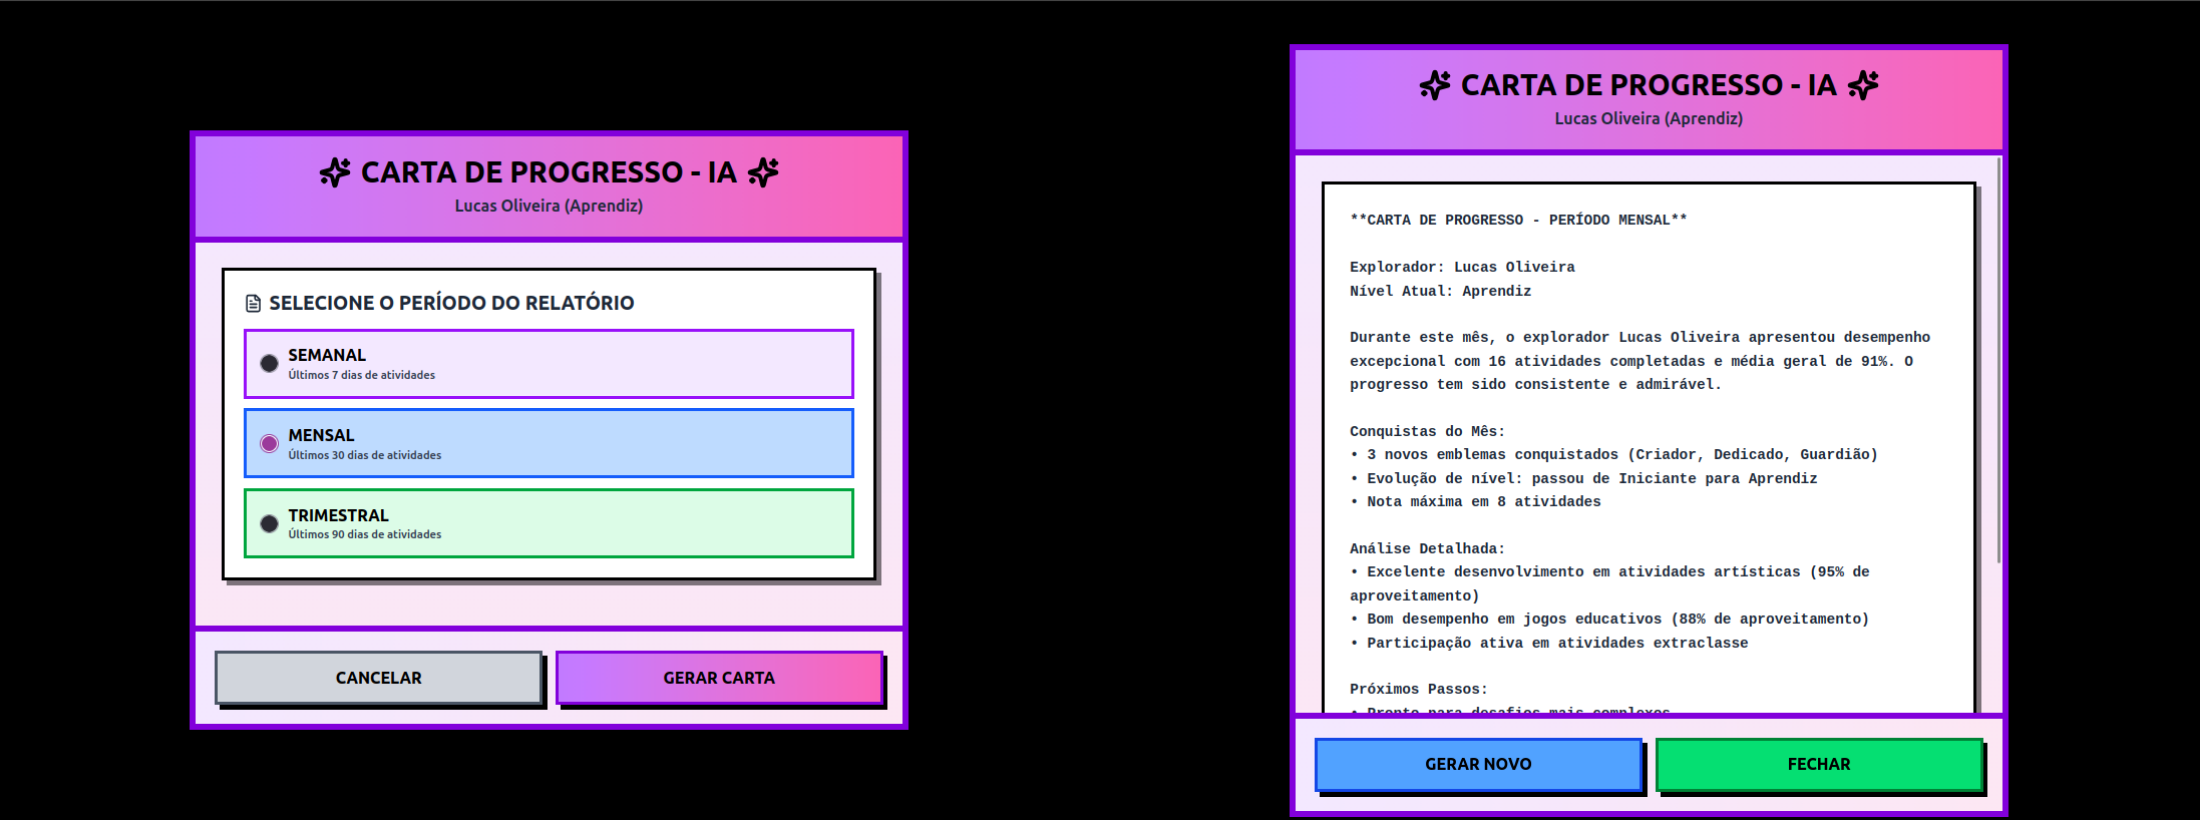
\includegraphics[width=0.75\textwidth]{adm05_carta_ia_periodo.png}
  \caption*{\small\textit{Fonte: Autoria própria, 2026.}}
\end{figure}
\textbf{Carta de Progresso IA --- Seleção de Período:} Interface modal que parametriza a
chamada ao serviço de Inteligência Artificial, permitindo ao Mestre da Jornada definir o
intervalo de análise (Semanal, Mensal ou Trimestral) antes de acionar a geração do relatório
personalizado do explorador. Esta tela atua como um objeto de controle que garante que a
Carta de Progresso seja elaborada com o escopo temporal correto conforme a necessidade
pedagógica.
 
\textbf{Carta de Progresso IA --- Resultado Gerado:} Exibe o texto personalizado produzido
pela Inteligência Artificial com base no histórico de conquistas do explorador, traduzindo
dados quantitativos em uma narrativa acolhedora direcionada aos responsáveis. A interface
apresenta o conteúdo em formato de documento estruturado, cobrindo conquistas do período,
análise por categoria de atividade e próximos passos sugeridos, encerrando o ciclo de
comunicação entre o sistema e a família do aluno.
 
\begin{figure}[H]
  \centering
  \caption*{Figura 20: Criar Tarefas por Atividade --- Lista de Missões.}
  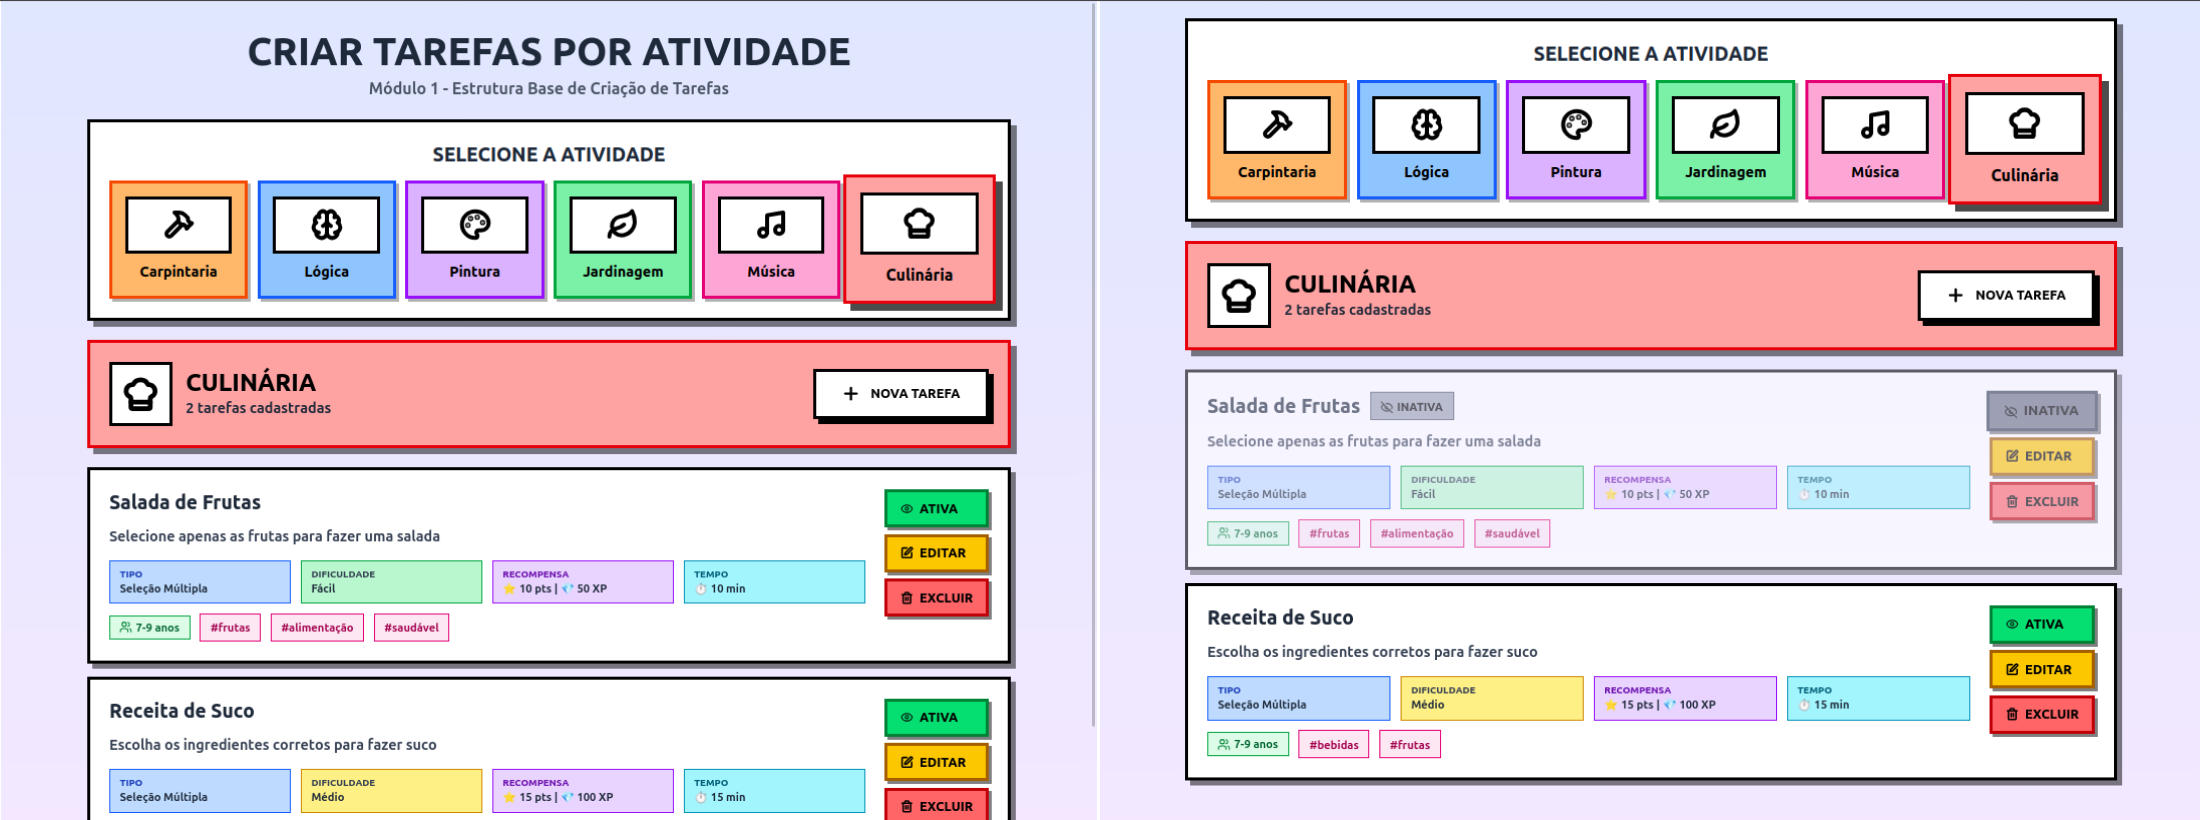
\includegraphics[width=0.85\textwidth]{adm10_criar_tarefas.png}
  \caption*{\small\textit{Fonte: Autoria própria, 2026.}}
\end{figure}
\textbf{Criar Tarefas por Atividade --- Lista de Missões:} Interface de listagem que exibe
as tarefas cadastradas para a categoria selecionada, permitindo ao Mestre da Jornada
visualizar os parâmetros de cada missão (tipo, dificuldade, recompensa, tempo e
\textit{tags}) e acionar operações de criação, edição ou exclusão. O status de cada tarefa
(Ativa ou Inativa) é exibido de forma destacada, permitindo ao professor controlar quais
atividades estão disponíveis para os exploradores sem precisar excluí-las do sistema.
 
\textbf{Gerenciar Tarefas --- Lista com Status Atualizado:} Apresenta o estado atual do
repositório de tarefas da categoria selecionada após operações de criação ou edição,
destacando visualmente a diferença entre tarefas Ativas (disponíveis aos exploradores) e
Inativas (suspensas). O Mestre pode alternar o status de cada tarefa sem excluí-la,
preservando o histórico de configurações e permitindo a reativação futura das missões.
\begin{figure}[H]
  \centering
  \caption*{Figura 21: Nova Tarefa --- Identificação, Configurações e Faixa Etária.}
  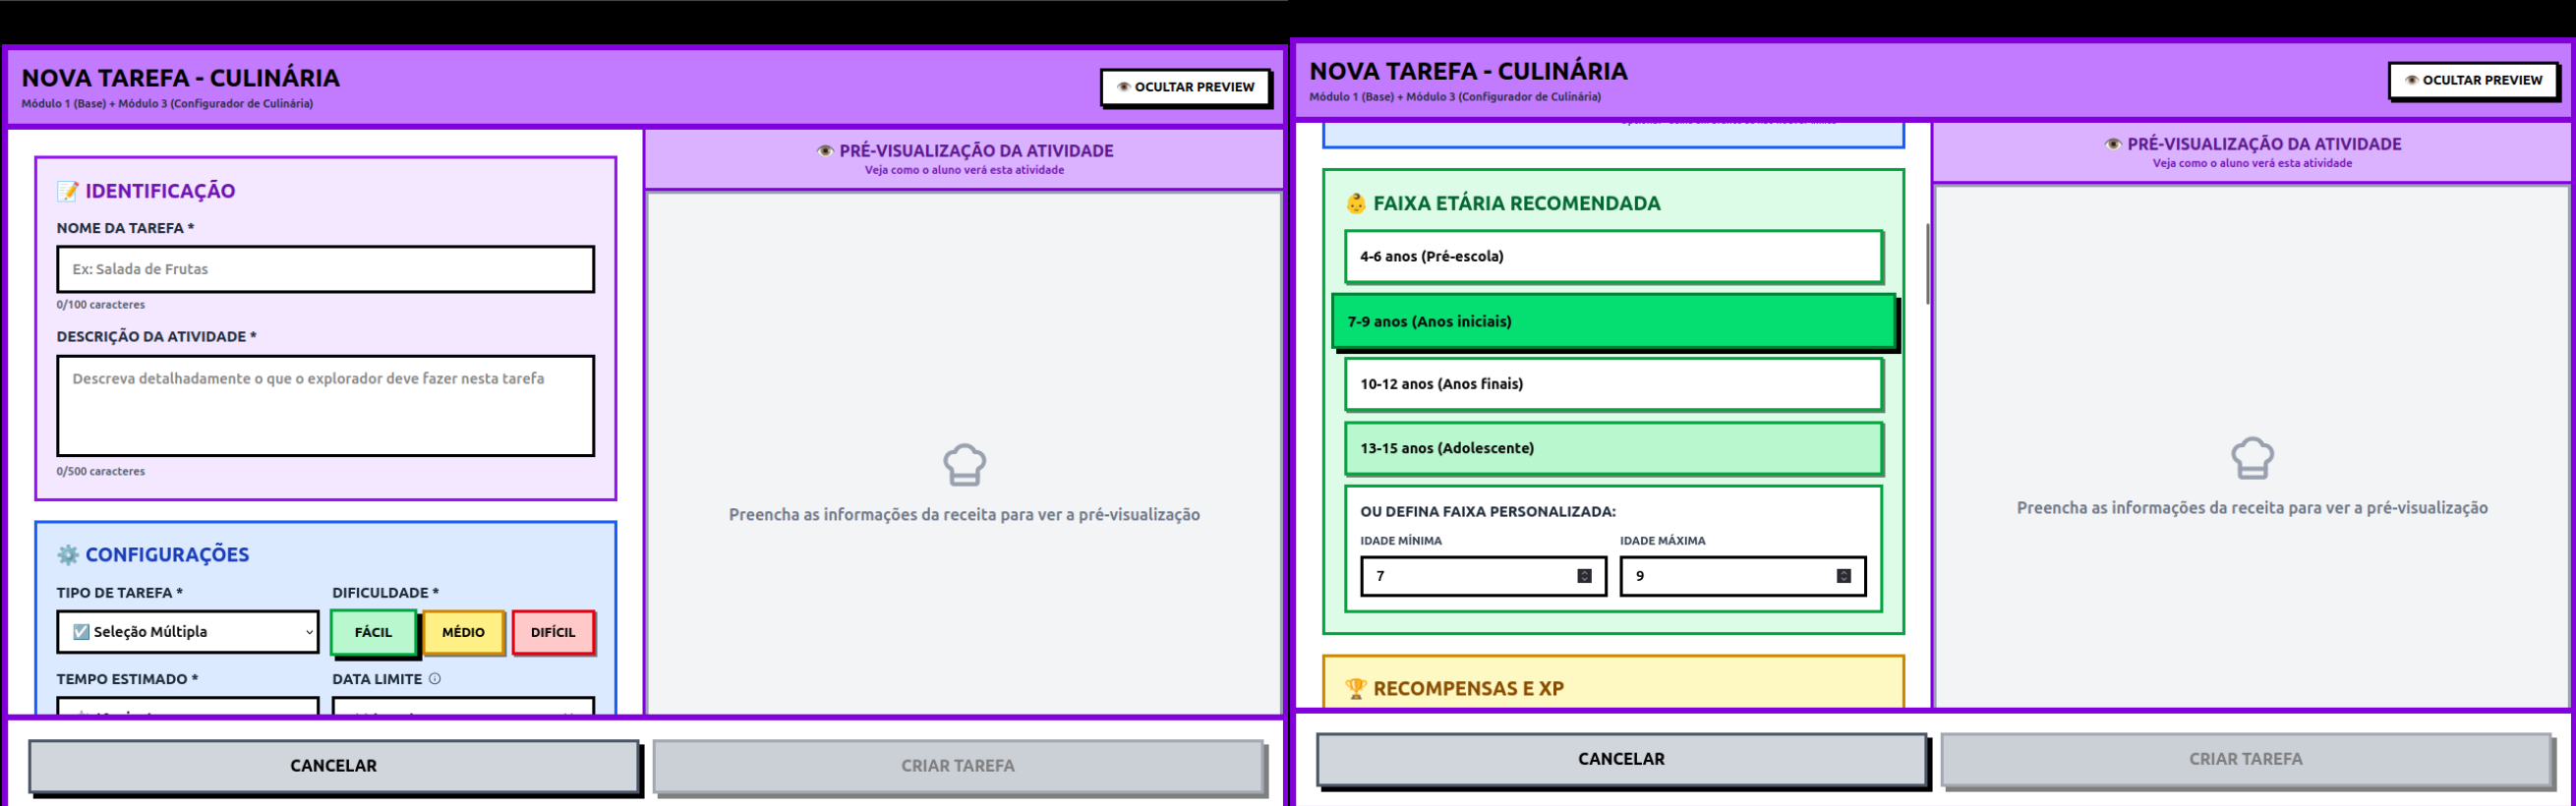
\includegraphics[width=0.85\textwidth]{adm12_nova_tarefa_identificacao2.png}
  \caption*{\small\textit{Fonte: Autoria própria, 2026.}}
\end{figure}
\textbf{Nova Tarefa --- Identificação e Configurações:} Tela de criação de missão que
solicita os metadados fundamentais do objeto \texttt{Missão}, como nome, descrição,
tipo de tarefa e nível de dificuldade (Fácil, Médio ou Difícil). A interface adota um
\textit{layout} dividido entre formulário de preenchimento e painel de pré-visualização ao
vivo, permitindo ao professor avaliar como a atividade será apresentada ao explorador antes
de confirmá-la no sistema.
 
\textbf{Nova Tarefa --- Faixa Etária Recomendada:} Esta seção do formulário de criação
define o público-alvo da missão por meio de opções predefinidas (4--6, 7--9, 10--12 e
13--15 anos) ou de uma faixa personalizada com campos de idade mínima e máxima. A
configuração da faixa etária permite ao sistema filtrar e recomendar tarefas adequadas ao
perfil de desenvolvimento de cada explorador, garantindo que os desafios pedagógicos sejam
sempre apropriados para a idade do usuário.
 
\begin{figure}[H]
  \centering
  \caption*{Figura 22: Nova Tarefa --- Recompensas, XP, \textit{Tags} e Configurador de Culinária}
  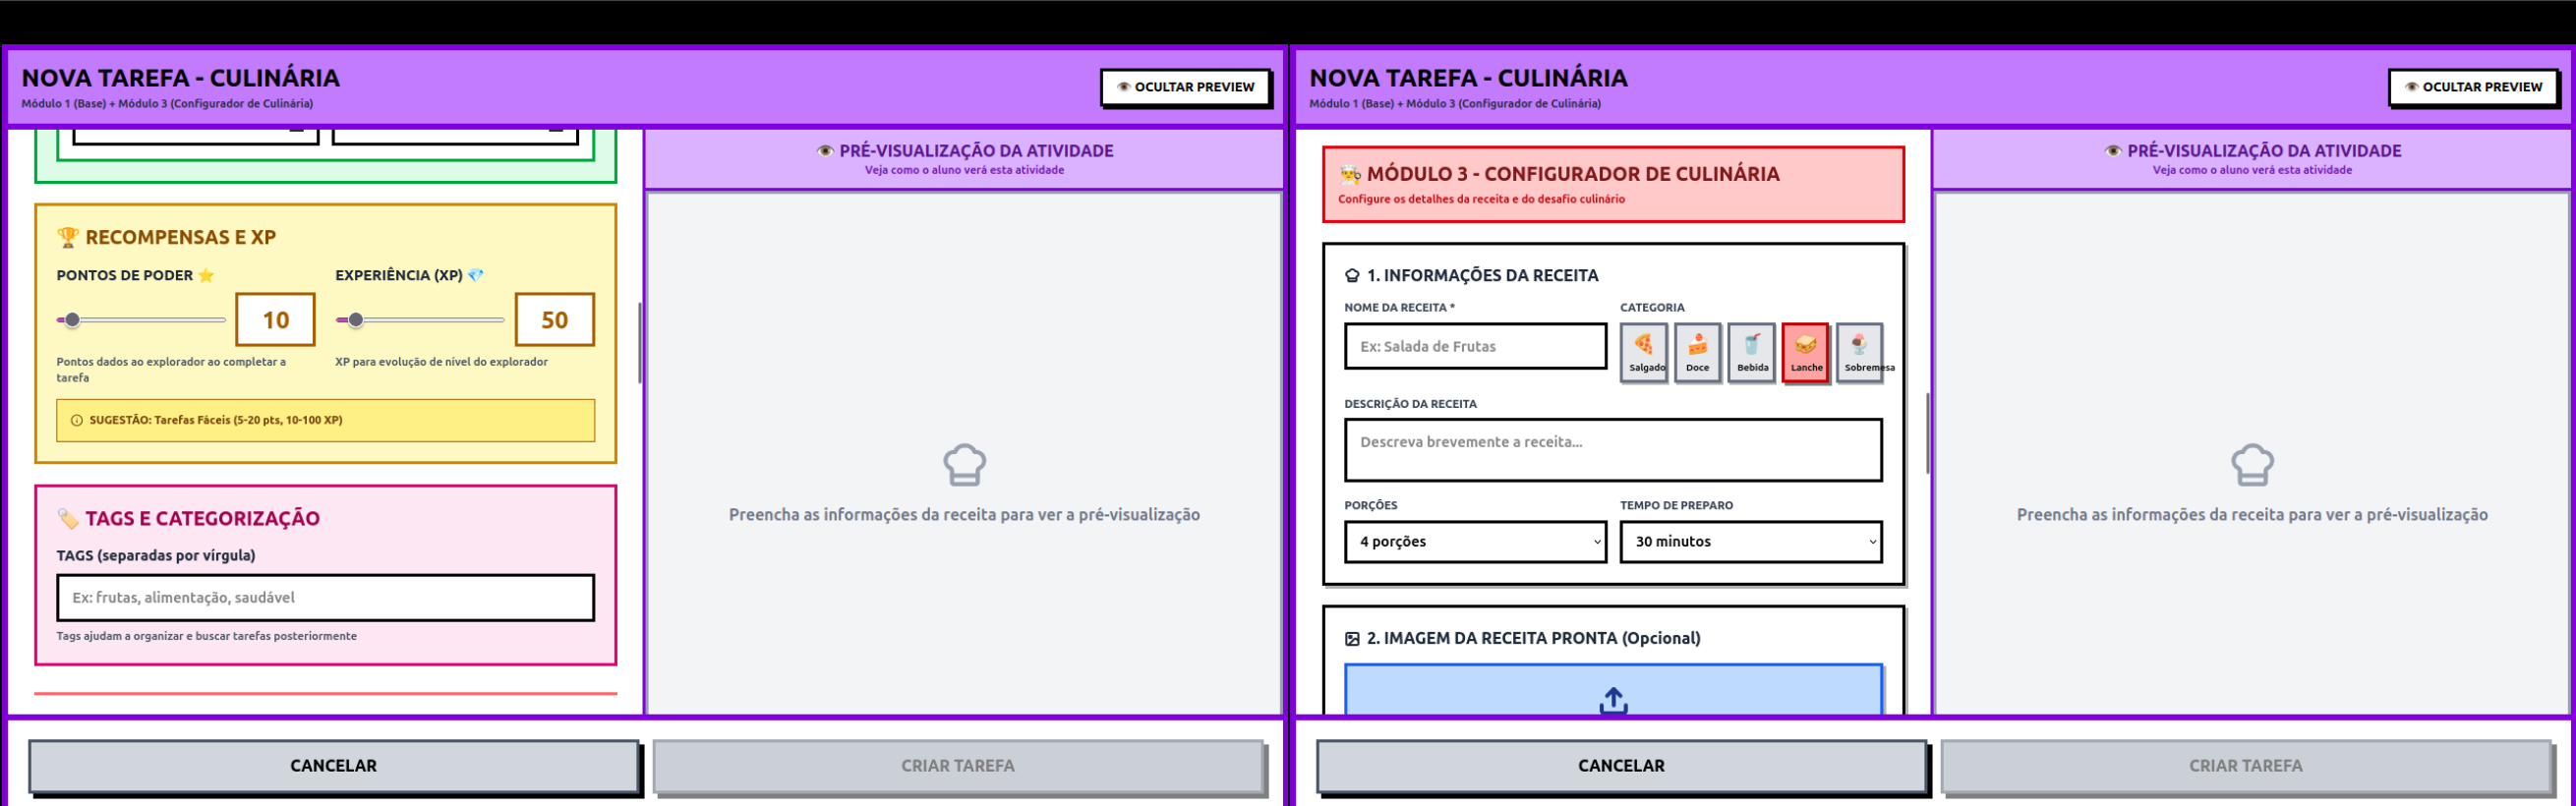
\includegraphics[width=0.85\textwidth]{adm14_nova_tarefa_recompensas.png}
  \caption*{\small\textit{Fonte: Autoria própria, 2026.}}
\end{figure}
\textbf{Nova Tarefa --- Recompensas, XP e \textit{Tags}:} Seção do formulário dedicada
à configuração do sistema de recompensas da missão, onde o Mestre define os Pontos de
Poder e a quantidade de Experiência (XP) concedidos ao explorador ao completar a tarefa,
com controles deslizantes e sugestões automáticas conforme o nível de dificuldade. O campo
de \textit{tags} complementa o cadastro com palavras-chave de categorização, facilitando a
busca e a organização pedagógica das tarefas no repositório do sistema.
 
\textbf{Nova Tarefa --- Módulo 3: Configurador de Culinária:} Este módulo especializado
complementa o formulário base com informações específicas da atividade culinária,
permitindo definir nome e descrição da receita, selecionar sua categoria (Salgado, Doce,
Bebida, Lanche ou Sobremesa) e configurar porções e tempo de preparo. A arquitetura
modular do formulário evidencia o padrão \textit{Decorator}, onde funcionalidades específicas
de cada categoria de atividade são adicionadas ao objeto base sem alterar sua estrutura
central.
 
\begin{figure}[H]
  \centering
  \caption*{Figura 23: Nova Tarefa --- Ingredientes e Modo de Preparo.}
  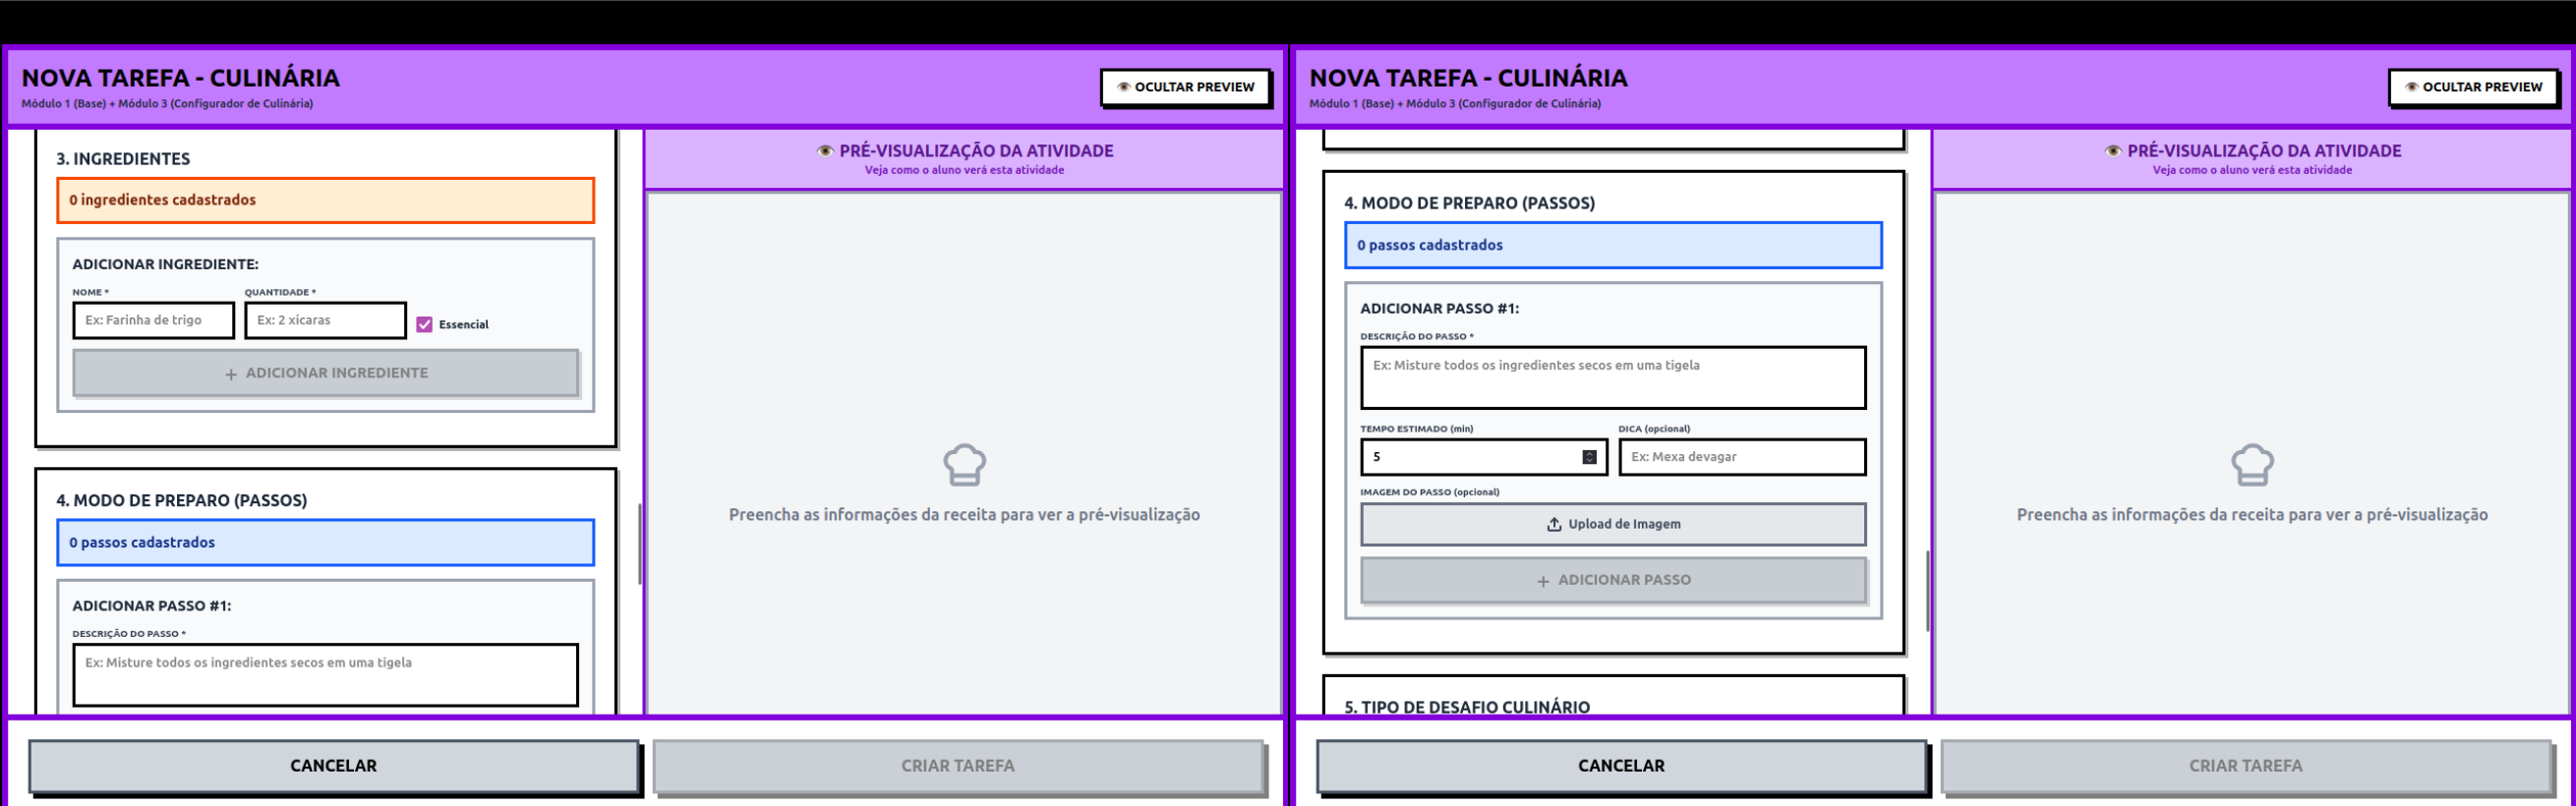
\includegraphics[width=0.85\textwidth]{adm16_nova_tarefa_ingredientes.png}
  \caption*{\small\textit{Fonte: Autoria própria, 2026.}}
\end{figure}
\textbf{Nova Tarefa --- Ingredientes e Modo de Preparo:} Esta seção gerencia as coleções
de objetos \texttt{Ingrediente} e \texttt{Passo} associados à receita, permitindo ao Mestre
adicionar itens individualmente com nome, quantidade e marcação de essencialidade. A
interface fornece \textit{feedback} imediato sobre o estado do cadastro, orientando o
preenchimento incremental e garantindo que a estrutura de dados da atividade esteja
completa antes da criação da tarefa no sistema.
 
\textbf{Nova Tarefa --- Cadastro de Passos do Preparo:} Permite ao Mestre detalhar cada
etapa do modo de preparo da receita, definindo descrição do passo, tempo estimado em
minutos, dica opcional e imagem ilustrativa. Cada entrada representa um objeto
\texttt{Passo} que compõe a lista sequencial do desafio culinário, enriquecendo a
experiência pedagógica com informações visuais e temporais que auxiliam o explorador
durante a execução da atividade.
 
\begin{figure}[H]
  \centering
  \caption*{Figura 24: Nova Tarefa --- Tipo de Desafio e Configurações Finais.}
  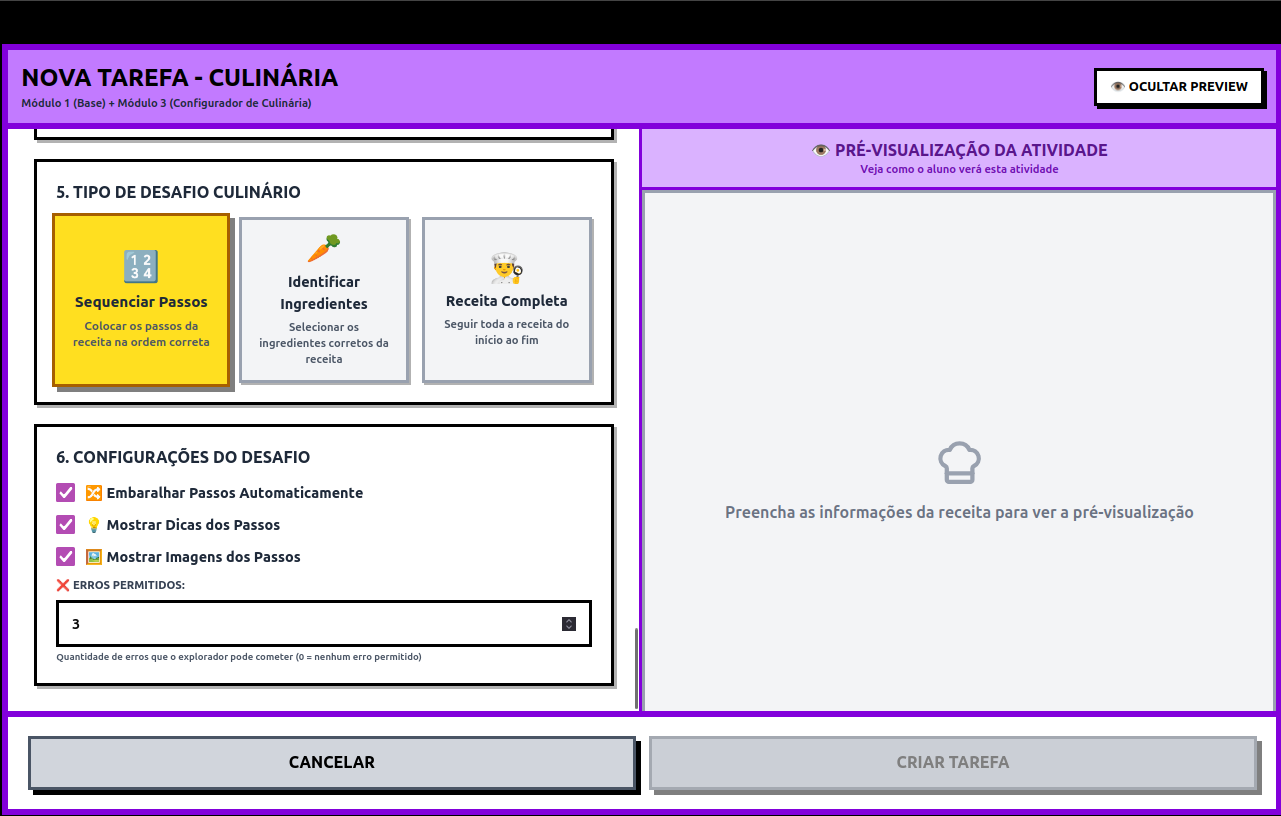
\includegraphics[width=0.85\textwidth]{adm18_nova_tarefa_desafio.png}
  \caption*{\small\textit{Fonte: Autoria própria, 2026.}}
\end{figure}
\textbf{Nova Tarefa --- Tipo de Desafio e Configurações Finais:} Etapa conclusiva do
formulário que define a mecânica de interação do desafio culinário, oferecendo três
modalidades: ``Sequenciar Passos'', ``Identificar Ingredientes'' e ``Receita Completa''. As
configurações adicionais permitem ajustar embaralhamento de passos, exibição de dicas e
imagens, e o número máximo de erros permitidos, personalizando o nível de dificuldade
operacional da missão.
 
\begin{figure}[H]
  \centering
  \caption*{Figura 25: Modal Editar Tarefa.}
  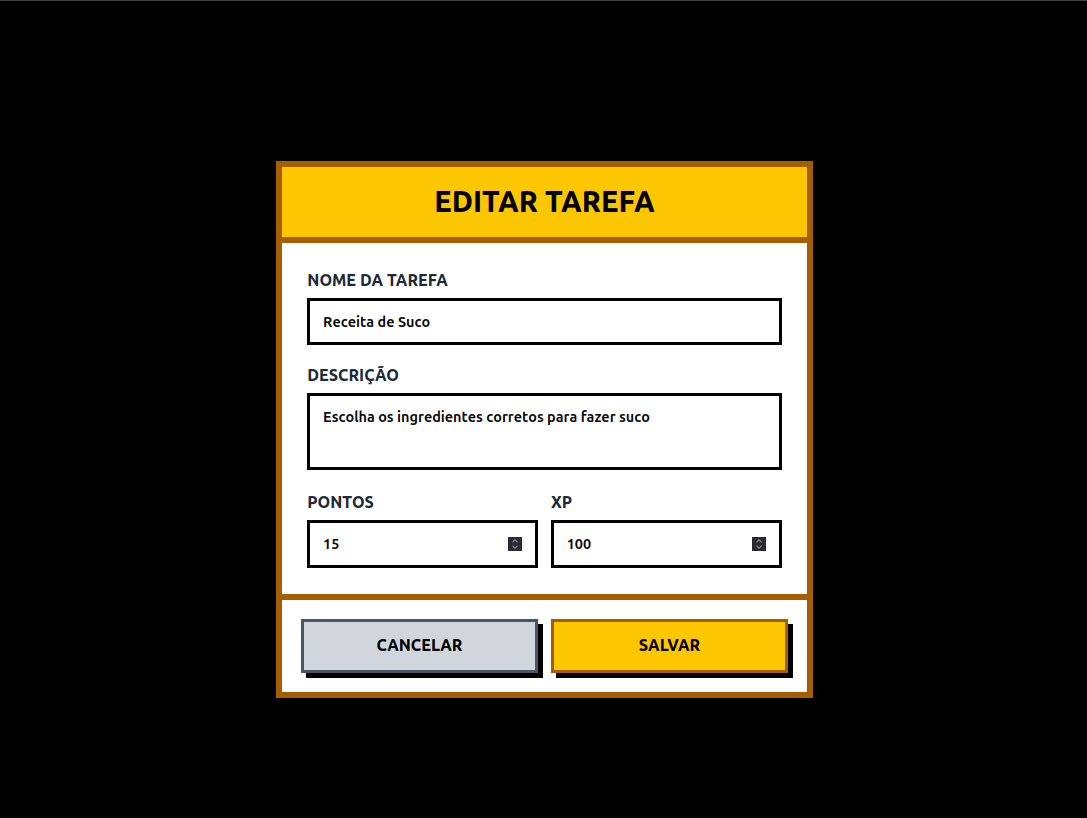
\includegraphics[width=0.75\textwidth]{adm20_editar_tarefa.png}
  \caption*{\small\textit{Fonte: Autoria própria, 2026.}}
\end{figure}
\textbf{Modal Editar Tarefa:} Interface modal compacta que permite ao Mestre da Jornada
atualizar os atributos essenciais de uma tarefa existente --- nome, descrição, pontos e XP
--- sem a necessidade de percorrer todo o fluxo de criação novamente. O modal atua como
um objeto de controle de edição rápida, reduzindo a fricção na manutenção do conteúdo
pedagógico e garantindo que ajustes pontuais possam ser aplicados de forma ágil.
 
\begin{figure}[H]
  \centering
  \caption*{Figura 26: Gerenciar Atividades Extraclasse.}
  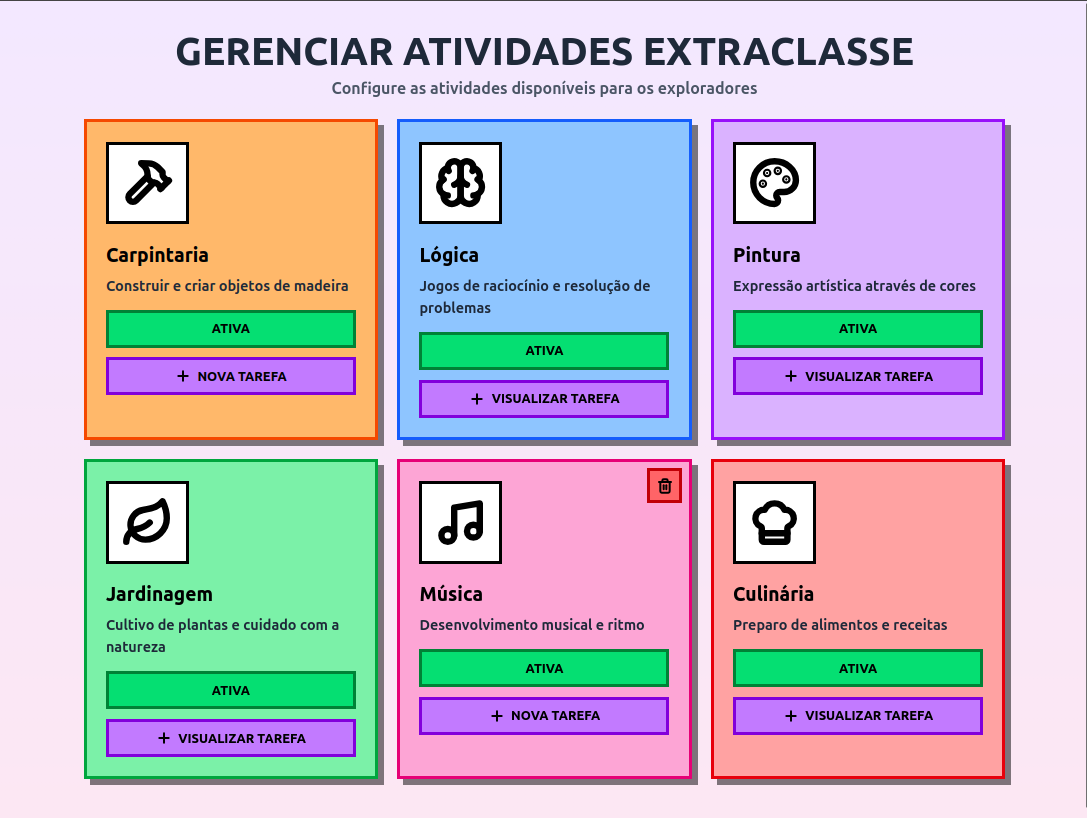
\includegraphics[width=0.85\textwidth]{adm21_extraclasse.png}
  \caption*{\small\textit{Fonte: Autoria própria, 2026.}}
\end{figure}
\textbf{Gerenciar Atividades Extraclasse:} Esta tela exibe o catálogo completo das
categorias de atividades disponíveis no sistema (Carpintaria, Lógica, Pintura, Jardinagem,
Música e Culinária), permitindo ao Mestre da Jornada visualizar o status de cada modalidade
e acessar diretamente a criação ou visualização de tarefas vinculadas. Cada cartão de
categoria funciona como um ponto de entrada para a gestão de conteúdo daquela disciplina
extracurricular, organizado de forma intuitiva e visualmente diferenciada por cores.
 
\begin{figure}[H]
  \centering
  \caption*{Figura 27: Gerenciar Emblemas.}
  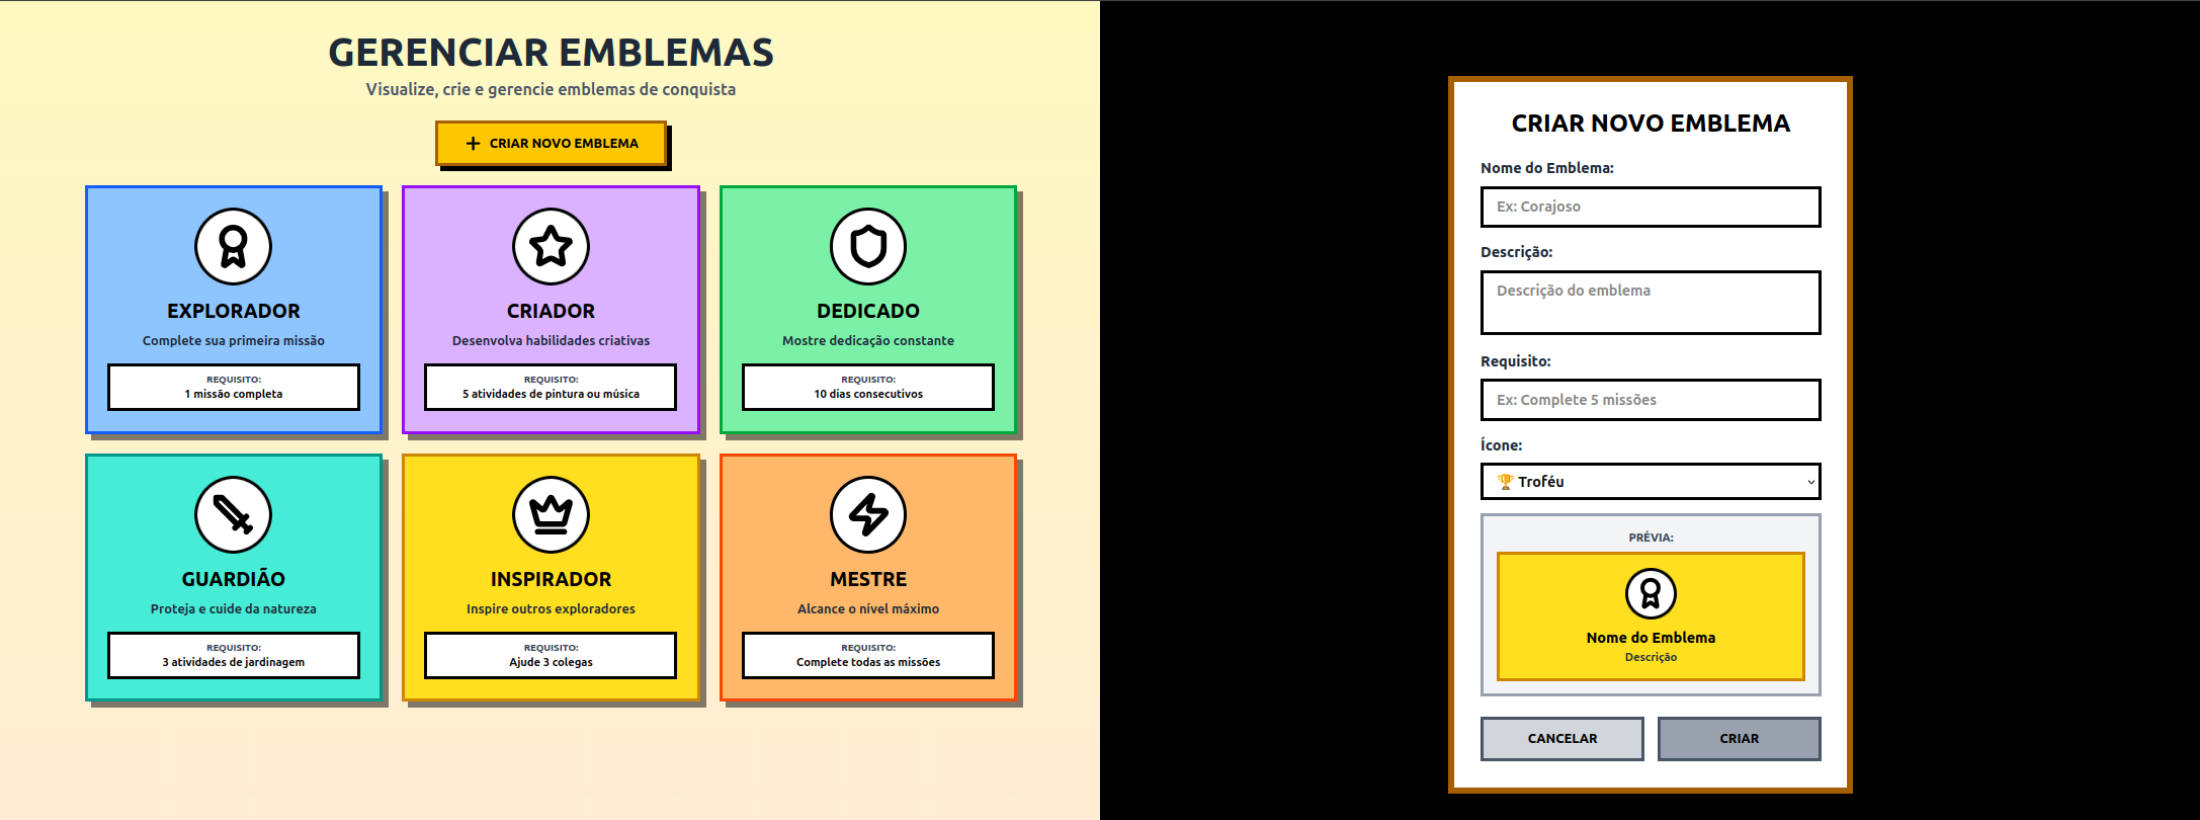
\includegraphics[width=0.85\textwidth]{adm22_emblemas_lista.png}
  \caption*{\small\textit{Fonte: Autoria própria, 2026.}}
\end{figure}
\textbf{Gerenciar Emblemas:} Interface que exibe o repositório de instâncias da classe
\texttt{Emblema} cadastradas no sistema, apresentando para cada conquista o nome, a
descrição motivacional e o requisito necessário para desbloqueá-la. A tela permite ao Mestre
criar novos emblemas, mantendo o catálogo de recompensas pedagógicas alinhado às metas
e progressões definidas no planejamento curricular do sistema gamificado.
 
\textbf{Modal Criar Novo Emblema:} Interface modal de cadastro que permite ao Mestre
instanciar um novo objeto \texttt{Emblema}, definindo nome, descrição, requisito de
desbloqueio e ícone representativo. A tela inclui um componente de pré-visualização que
renderiza em tempo real o cartão visual do emblema conforme os dados são inseridos,
garantindo que a aparência final da conquista seja validada antes de ser persistida no sistema.
 
\begin{figure}[H]
  \centering
  \caption*{Figura 28: Correção de Atividades --- Visualização Geral.}
  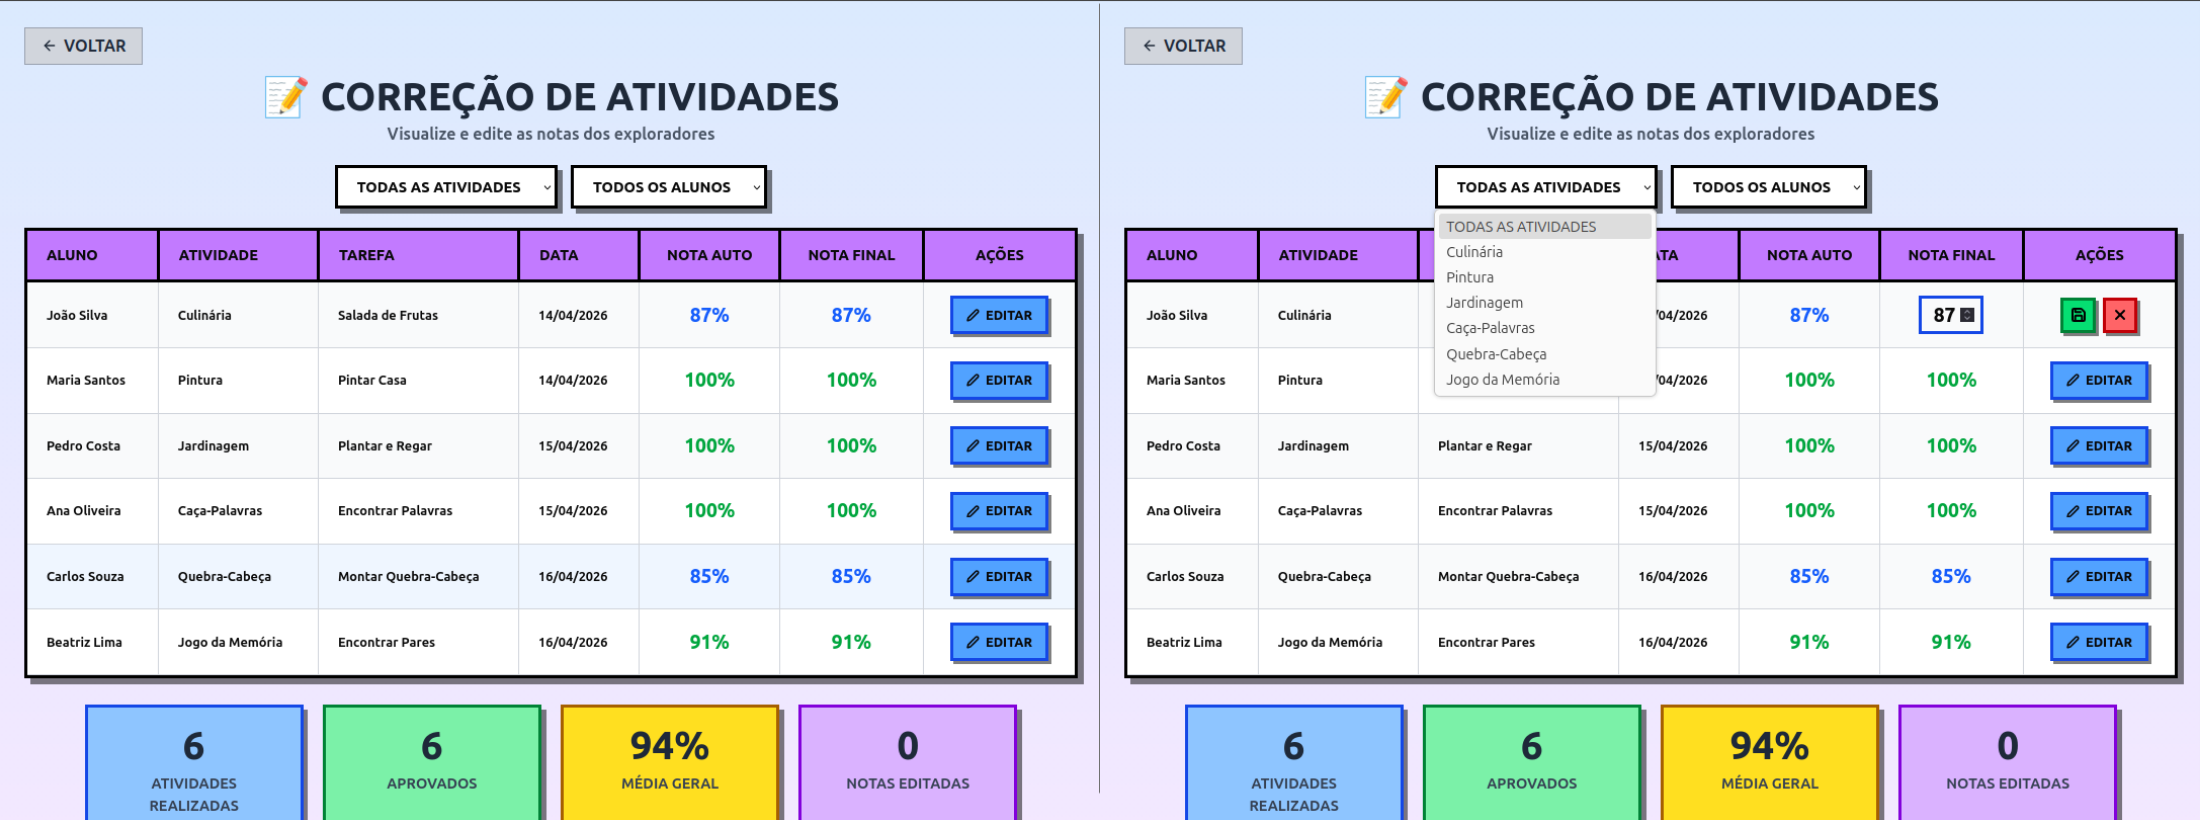
\includegraphics[width=0.85\textwidth]{adm25_correcao_lista.png}
  \caption*{\small\textit{Fonte: Autoria própria, 2026.}}
\end{figure}
\begin{figure}[H]
  \centering
  \caption*{Figura 29: Correção de Atividades --- Filtro por Atividade.}
  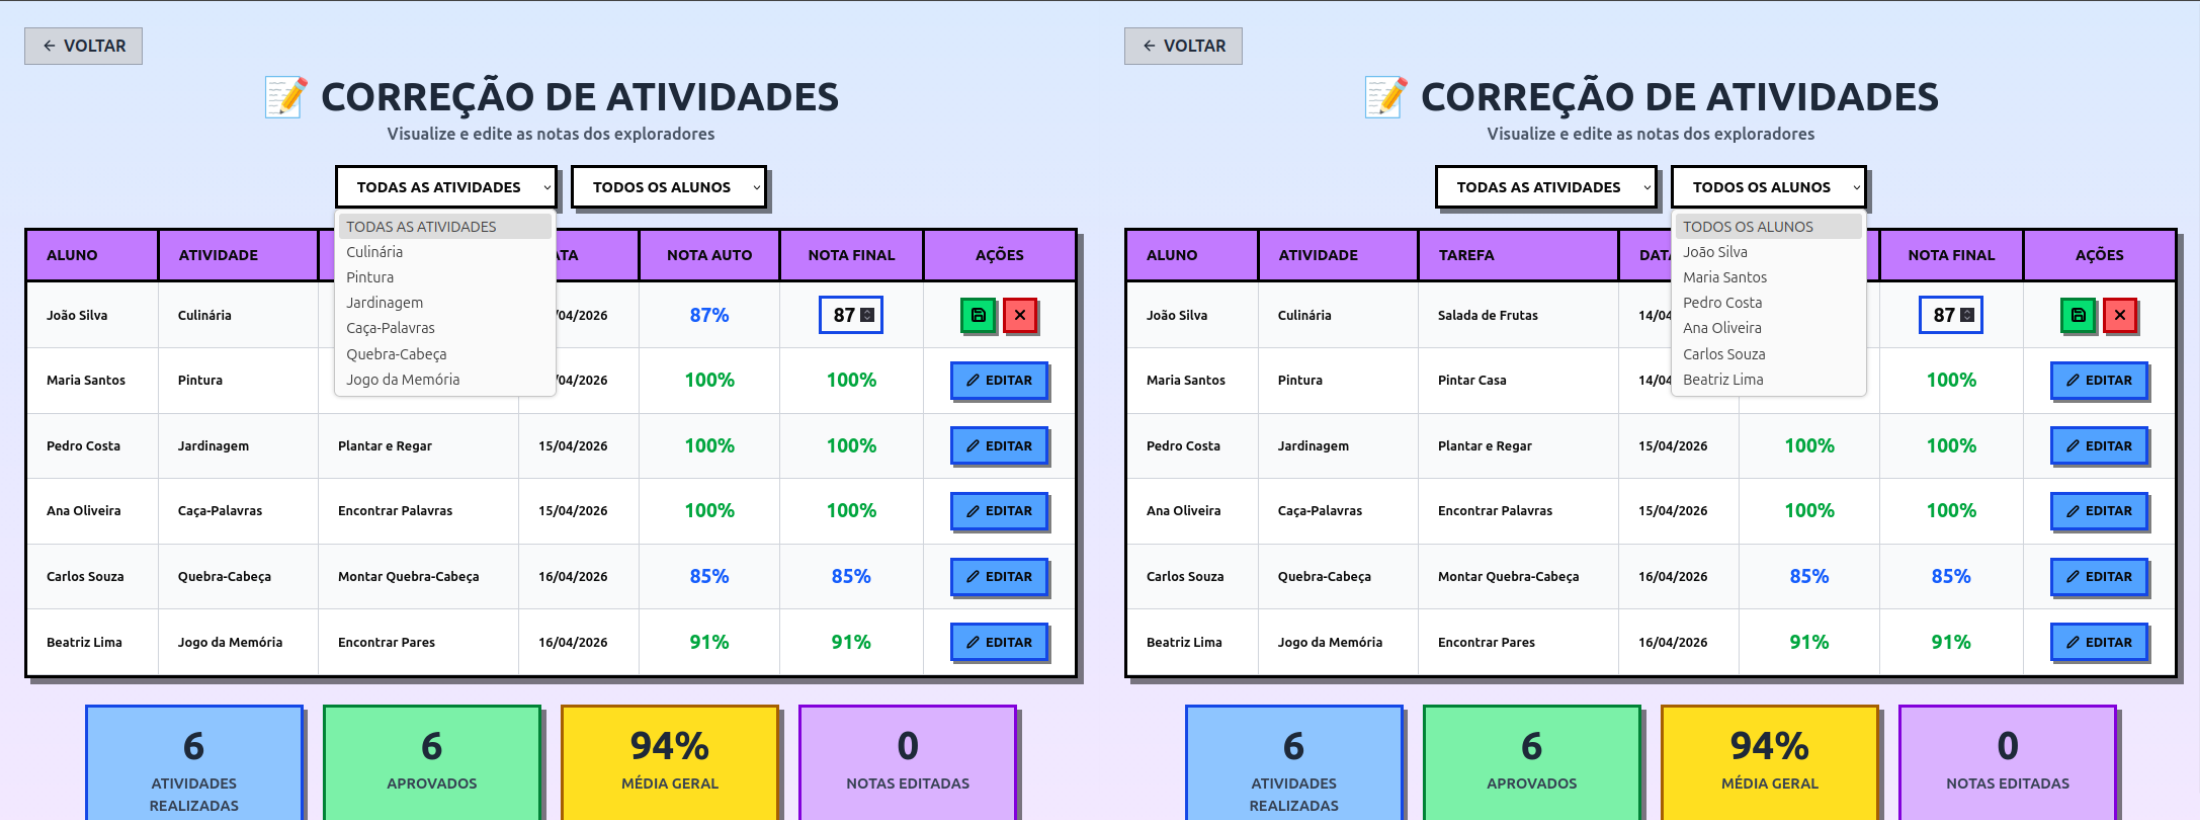
\includegraphics[width=0.85\textwidth]{adm27_correcao_filtro_atividade.png}
  \caption*{\small\textit{Fonte: Autoria própria, 2026.}}
\end{figure}
\textbf{Correção de Atividades:} Esta interface tabular centraliza o controle avaliativo do
Mestre da Jornada, exibindo para cada registro o aluno, a atividade, a tarefa, a data de
realização, a nota automática gerada pelo sistema e a nota final editável. O professor pode
sobrepor a avaliação automática com um julgamento qualitativo diretamente na célula da
tabela, enquanto os painéis de estatísticas na base fornecem indicadores agregados como
total de atividades realizadas, aprovados, média geral e notas editadas. Os filtros por
atividade e por aluno permitem segmentar a visualização para acompanhamentos
individualizados ou por modalidade pedagógica.
 
% --------------------------------------------------------------
\subsubsection{Guardião (Pedagogo)}
% --------------------------------------------------------------
 
\begin{figure}[H]
  \centering
  \caption*{Figura 30: Login Administrativo --- Formulário de Acesso (Guardião).}
  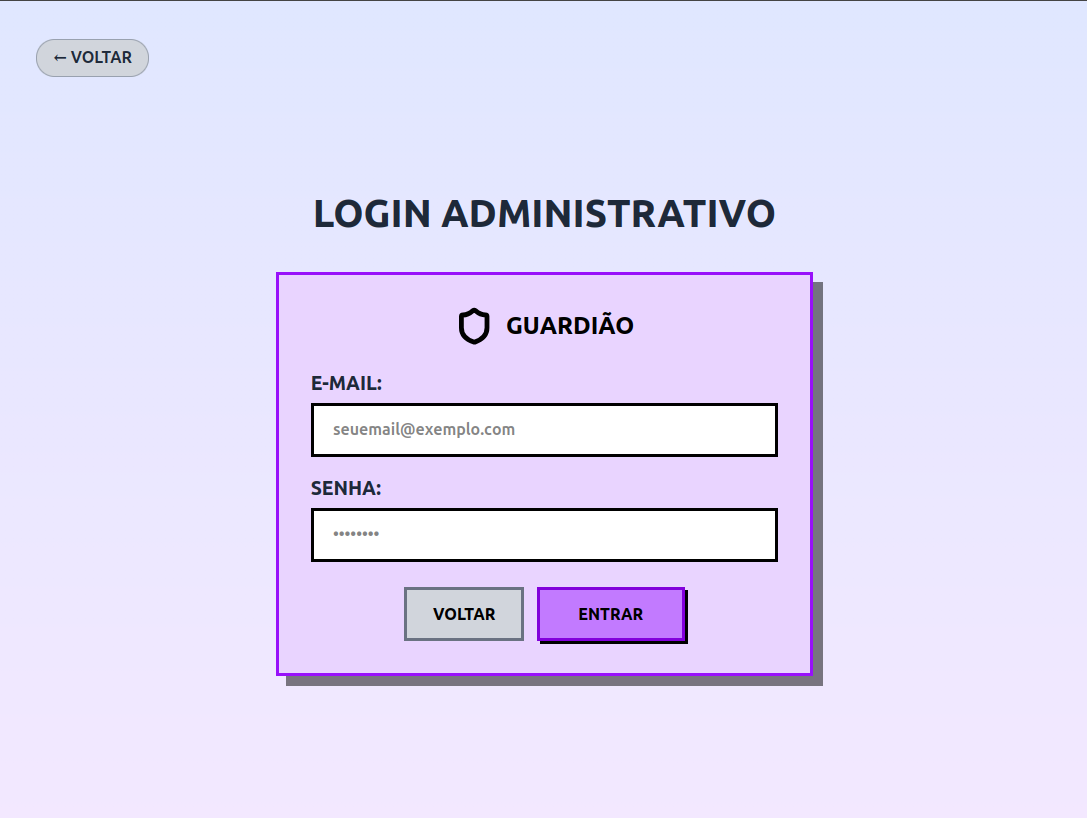
\includegraphics[width=0.85\textwidth]{adm29_login_guardiao.png}
  \caption*{\small\textit{Fonte: Autoria própria, 2026.}}
\end{figure}
\textbf{Login Administrativo --- Formulário de Acesso (Guardião):} Espelhando
estruturalmente o login do Mestre da Jornada, esta tela autentica o perfil \texttt{Guardião}
(pedagogo) por meio de e-mail e senha, distinguindo-se pelo esquema de cores roxo e pelo
ícone de escudo que reforça visualmente o nível de privilégio elevado deste papel. Após a
validação, o Guardião é direcionado à Área Administrativa, que concentra as funções de
cadastro e supervisão global do sistema.
 
\begin{figure}[H]
  \centering
  \caption*{Figura 31: Área Administrativa --- Painel do Guardião.}
  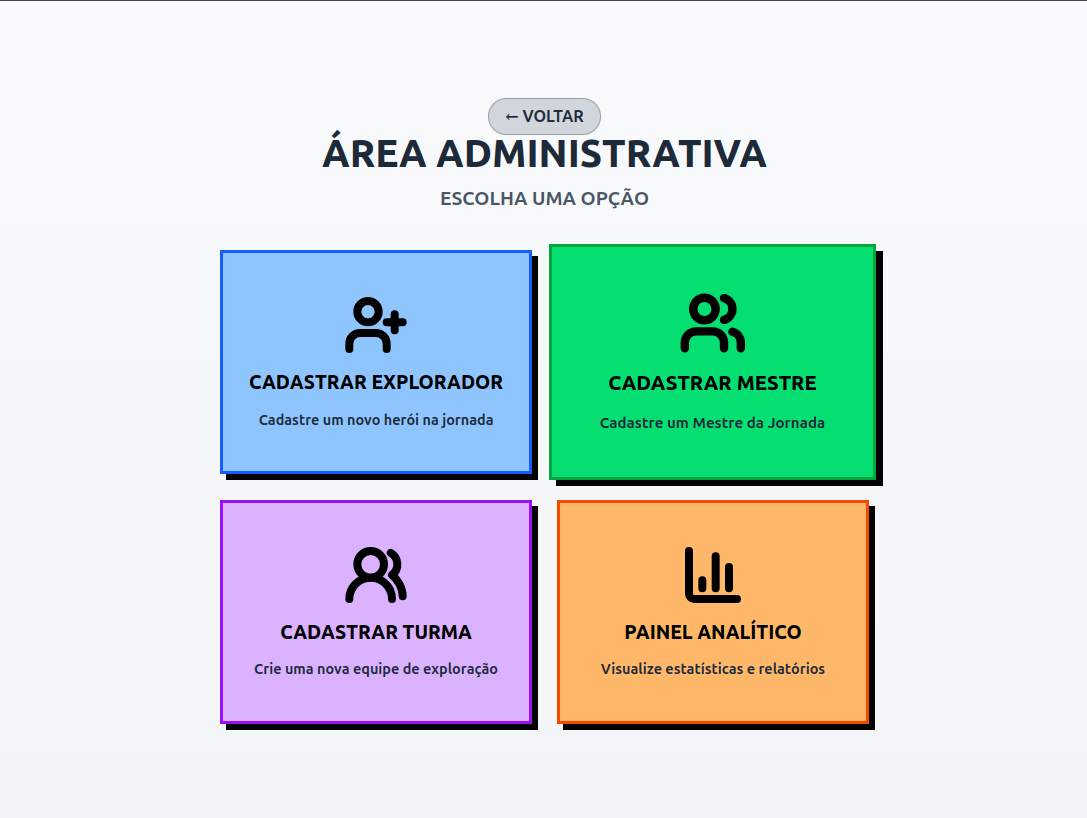
\includegraphics[width=0.85\textwidth]{adm30_area_administrativa.png}
  \caption*{\small\textit{Fonte: Autoria própria, 2026.}}
\end{figure}
\textbf{Área Administrativa --- Painel do Guardião:} Atua como o dashboard central do
perfil de mais alto privilégio no sistema, disponibilizando acesso direto aos módulos de
Cadastrar Explorador, Cadastrar Mestre, Cadastrar Turma e Painel Analítico. A interface
organiza essas responsabilidades em uma grade de quatro cartões coloridos e
autoexplicativos, permitindo ao Guardião supervisionar a estrutura pedagógica e
populacional da plataforma com acesso centralizado a todas as operações de gestão global.
 
\begin{figure}[H]
  \centering
  \caption*{Figura 32: Cadastro de Explorador --- Formulário (parte superior).}
  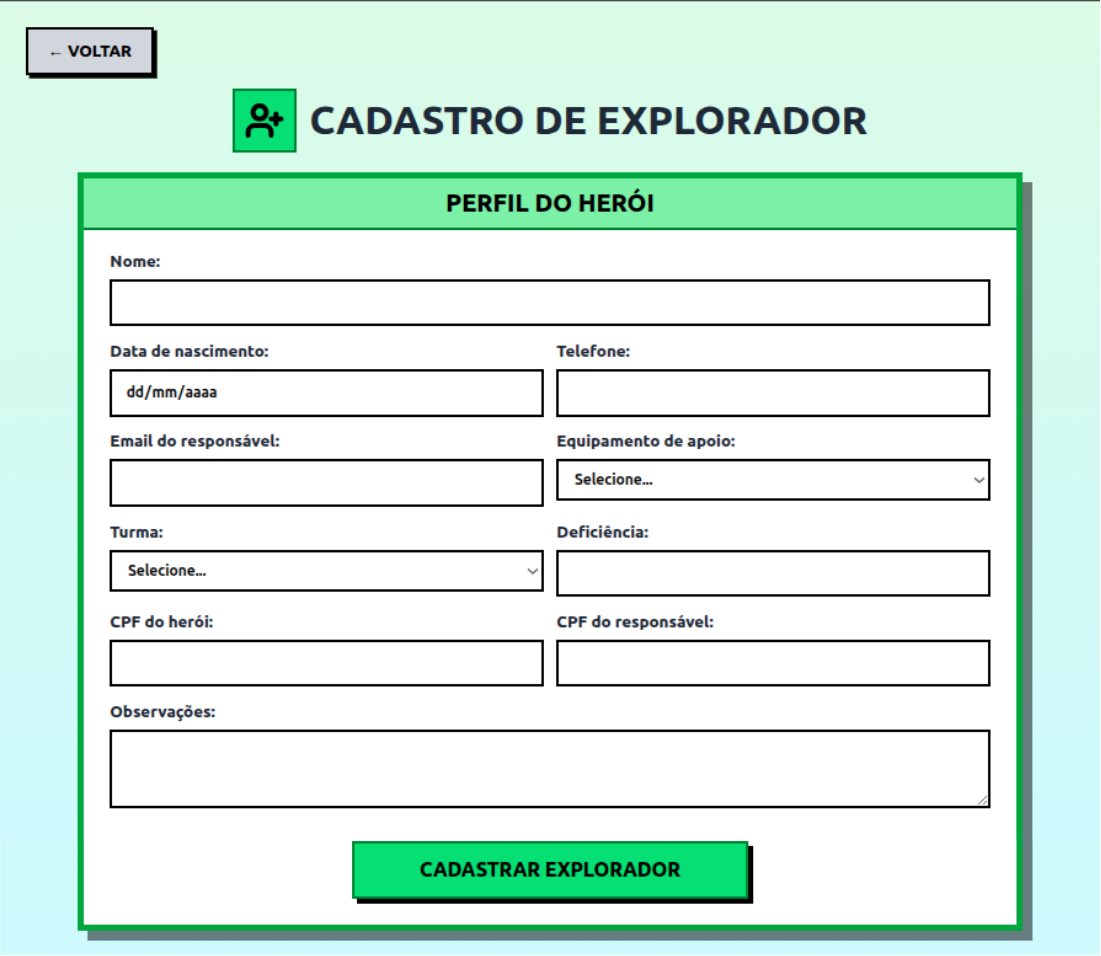
\includegraphics[width=0.85\textwidth]{adm31_cadastro_explorador1.png}
  \caption*{\small\textit{Fonte: Autoria própria, 2026.}}
\end{figure}
\textbf{Cadastro de Explorador --- Perfil do Herói:} Interface de formulário completo
responsável pela criação de um novo objeto \texttt{Explorador} no sistema, consolidando
em uma única tela todos os atributos essenciais: nome, data de nascimento, telefone, e-mail
do responsável, equipamento de apoio, turma, deficiência, CPFs do herói e do responsável,
e observações pedagógicas. O campo de equipamento de apoio integra diretamente a
classe \texttt{Acessibilidade}, garantindo que as necessidades especiais do aluno sejam
capturadas no momento da matrícula para configurar automaticamente sua experiência
no sistema.
 
\begin{figure}[H]
  \centering
  \caption*{Figura 33: Cadastro de Explorador --- Confirmação de Sucesso.}
  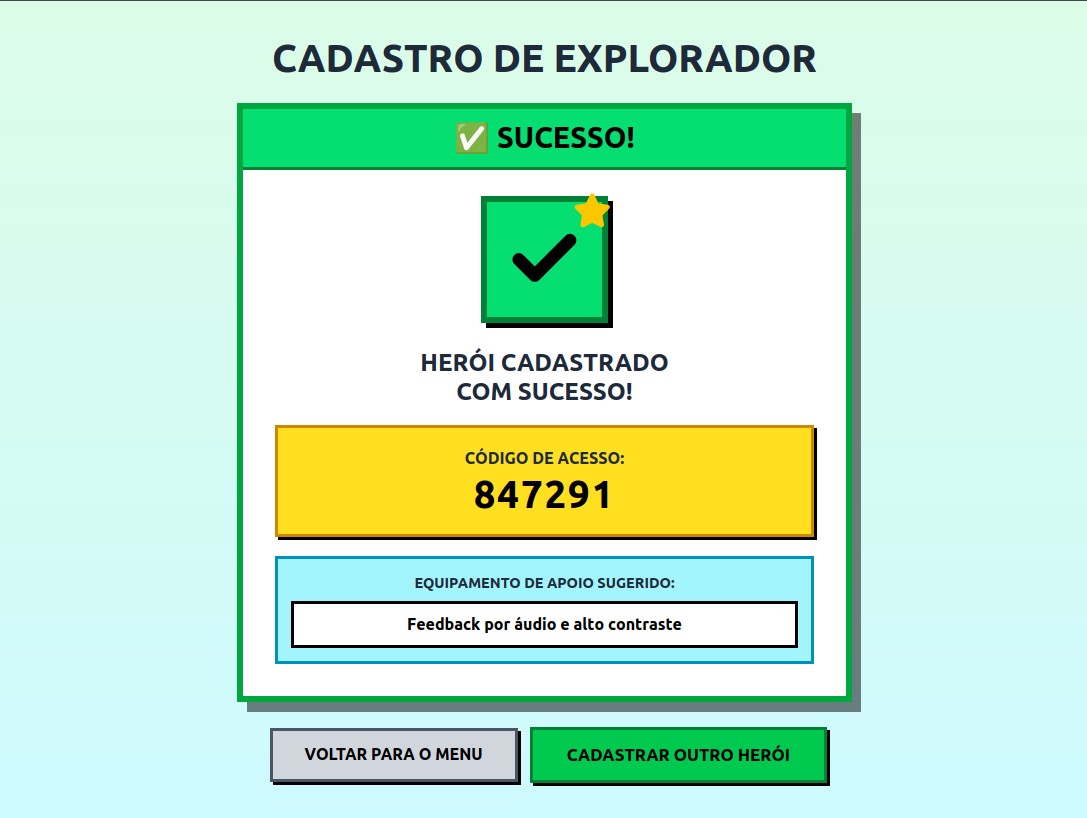
\includegraphics[width=0.85\textwidth]{adm34_cadastro_explorador_sucesso.png}
  \caption*{\small\textit{Fonte: Autoria própria, 2026.}}
\end{figure}
\textbf{Cadastro de Explorador --- Confirmação de Sucesso:} Tela de retorno que confirma
a persistência bem-sucedida do objeto \texttt{Explorador} no banco de dados e exibe
imediatamente o Código de Acesso gerado automaticamente pelo sistema, juntamente com
o Equipamento de Apoio sugerido com base no perfil de acessibilidade informado. Esta
interface encerra o fluxo de cadastro fornecendo ao Guardião as credenciais físicas que
serão entregues ao aluno, garantindo rastreabilidade e imediata operacionalidade da
identidade digital criada.
 
\begin{figure}[H]
  \centering
  \caption*{Figura 34: Cadastro de Mestre da Jornada --- Formulário.}
  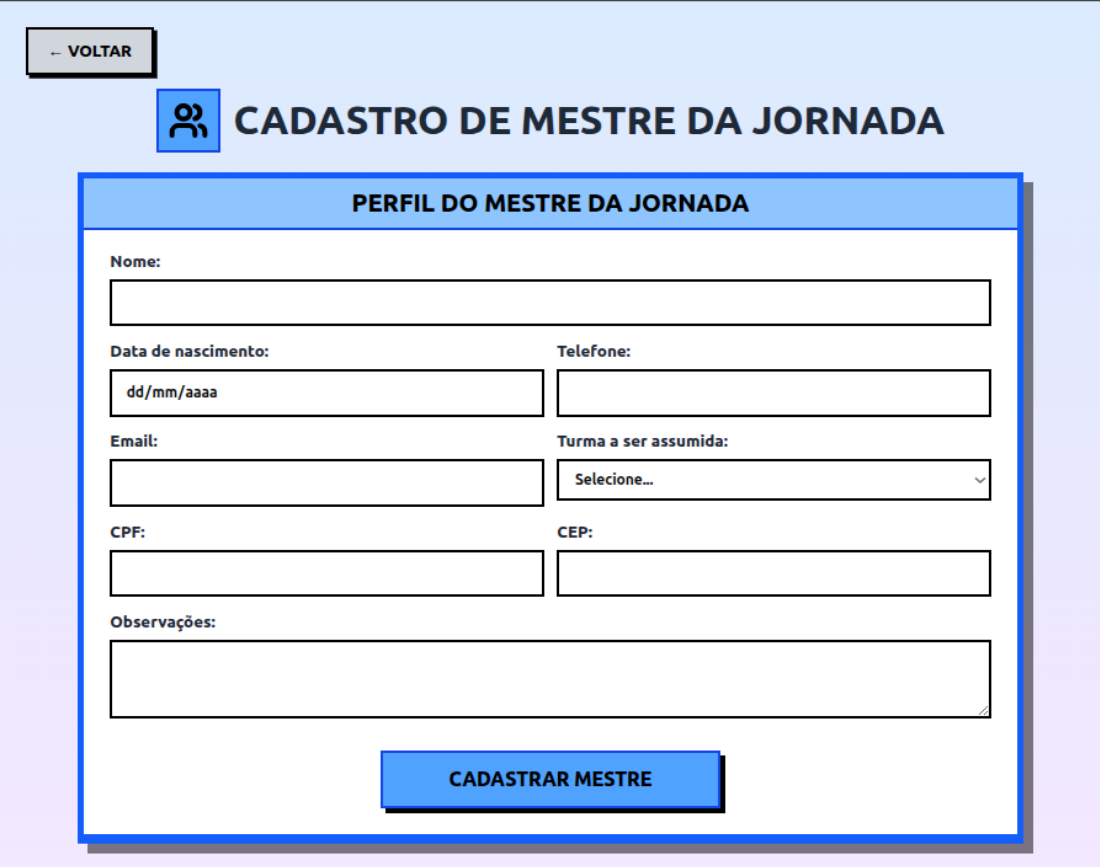
\includegraphics[width=0.85\textwidth]{adm33_cadastro_mestre.png}
  \caption*{\small\textit{Fonte: Autoria própria, 2026.}}
\end{figure}
\textbf{Cadastro de Mestre da Jornada --- Perfil do Mestre:} Interface de formulário
dedicada à criação de um novo objeto \texttt{MestreJornada} no sistema, coletando atributos
como nome, data de nascimento, telefone, e-mail, turma a ser assumida, CPF, CEP e
observações. O campo ``Turma a ser assumida'' realiza a associação direta entre o professor
e sua classe de exploradores já no ato do cadastro, simplificando a configuração inicial da
estrutura pedagógica e garantindo que o Mestre possa acessar seu painel imediatamente
após a ativação da conta.
 
\begin{figure}[H]
  \centering
  \caption*{Figura 35: Cadastro de Mestre da Jornada --- Confirmação de Sucesso.}
  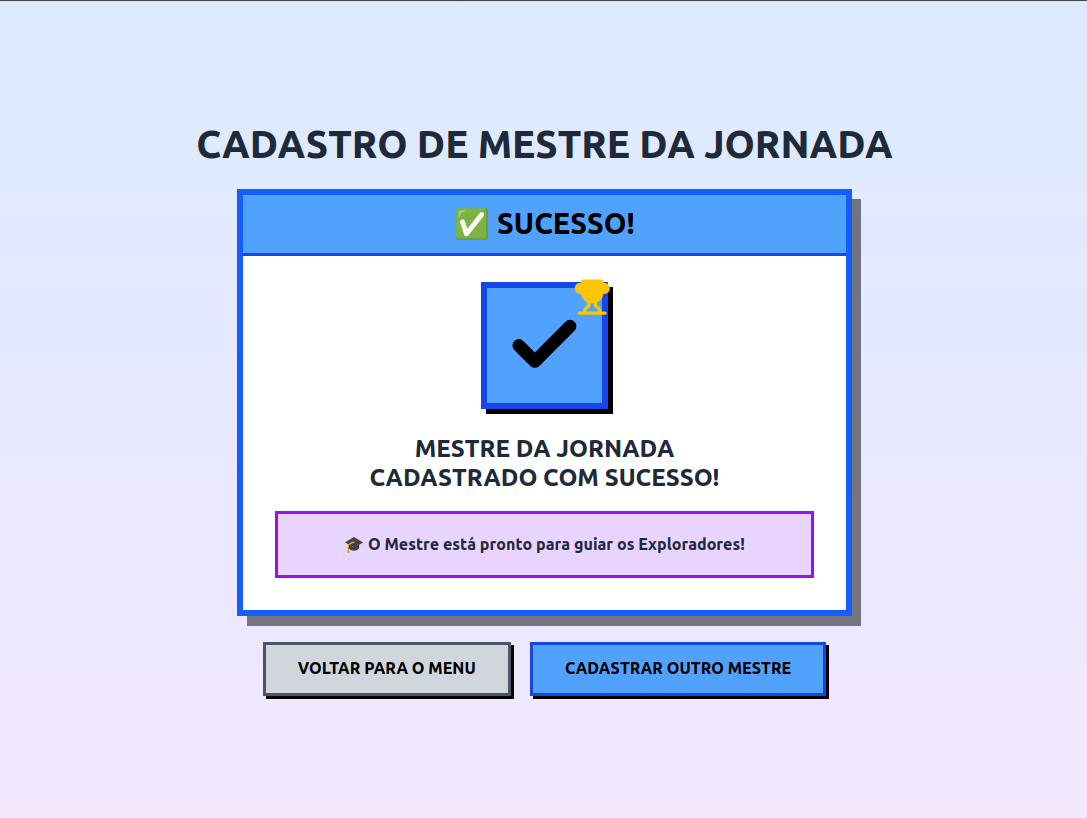
\includegraphics[width=0.85\textwidth]{adm35_cadastro_mestre_sucesso.png}
  \caption*{\small\textit{Fonte: Autoria própria, 2026.}}
\end{figure}
\textbf{Cadastro de Mestre da Jornada --- Confirmação de Sucesso:} Tela de retorno que
confirma o registro bem-sucedido do professor no sistema por meio de \textit{feedback}
visual positivo, informando que o Mestre está pronto para guiar os Exploradores. A interface
oferece ações de continuidade para retornar ao menu administrativo ou cadastrar outro
Mestre, encerrando o fluxo de onboarding do professor e tornando sua conta imediatamente
disponível para autenticação no sistema.
 
\begin{figure}[H]
  \centering
  \caption*{Figura 36: Cadastro de Turma --- Configuração da Equipe (parte superior).}
  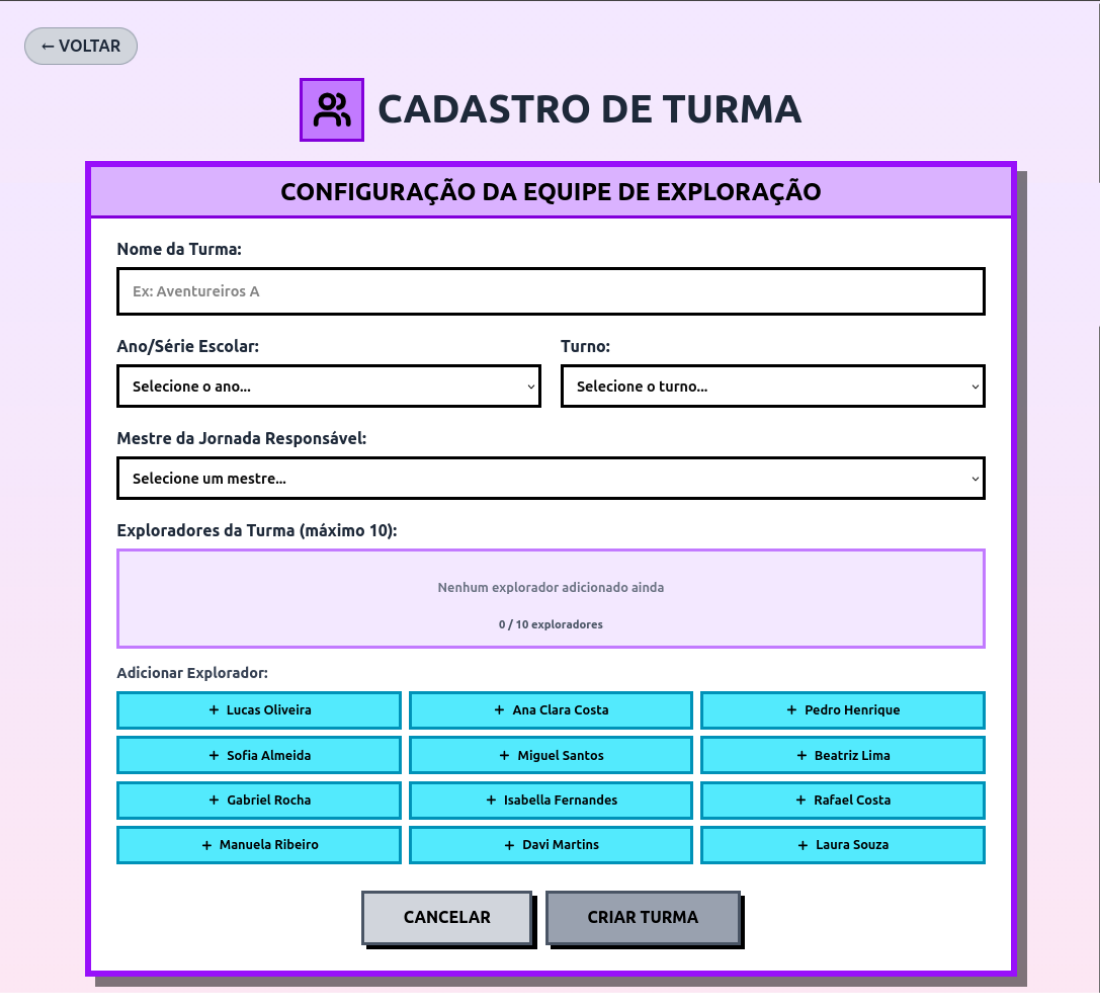
\includegraphics[width=0.85\textwidth]{adm36_cadastro_turma1.png}
  \caption*{\small\textit{Fonte: Autoria própria, 2026.}}
\end{figure}
\textbf{Cadastro de Turma --- Configuração da Equipe de Exploração:} Interface de
formulário responsável pela criação de um novo objeto \texttt{Turma}, solicitando nome da
turma, ano/série escolar, turno e Mestre da Jornada responsável, além de permitir a adição
imediata de exploradores ao grupo mediante clique nos botões de cada aluno disponível.
A tela mantém o contador de exploradores adicionados em tempo real (0/10), garantindo
que o limite máximo seja respeitado e que a composição inicial da equipe seja definida já
no momento da criação da turma pelo Guardião.
 
\begin{figure}[H]
  \centering
  \caption*{Figura 37: Painel Analítico Geral --- Visão Inicial (sem turma selecionada).}
  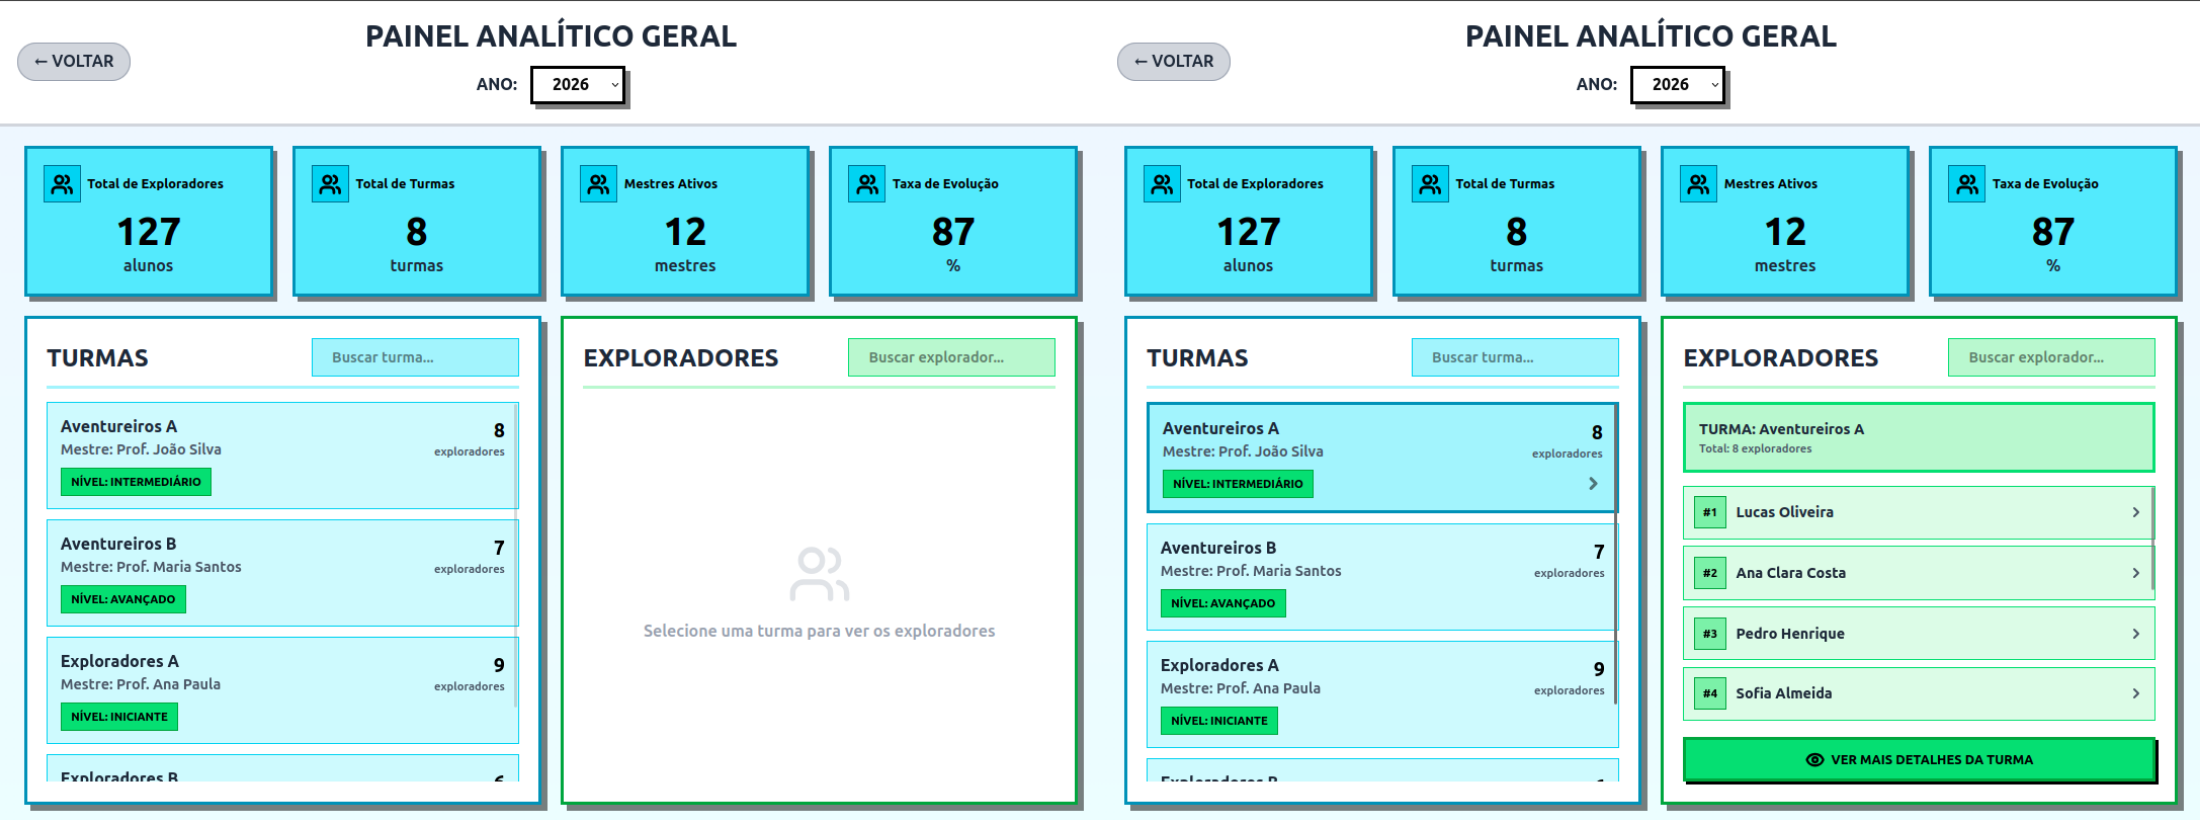
\includegraphics[width=0.85\textwidth]{adm38_painel_analitico1.png}
  \caption*{\small\textit{Fonte: Autoria própria, 2026.}}
\end{figure}
\begin{figure}[H]
  \centering
  \caption*{Figura 38: Painel Analítico Geral --- Filtro por Ano Letivo.}
  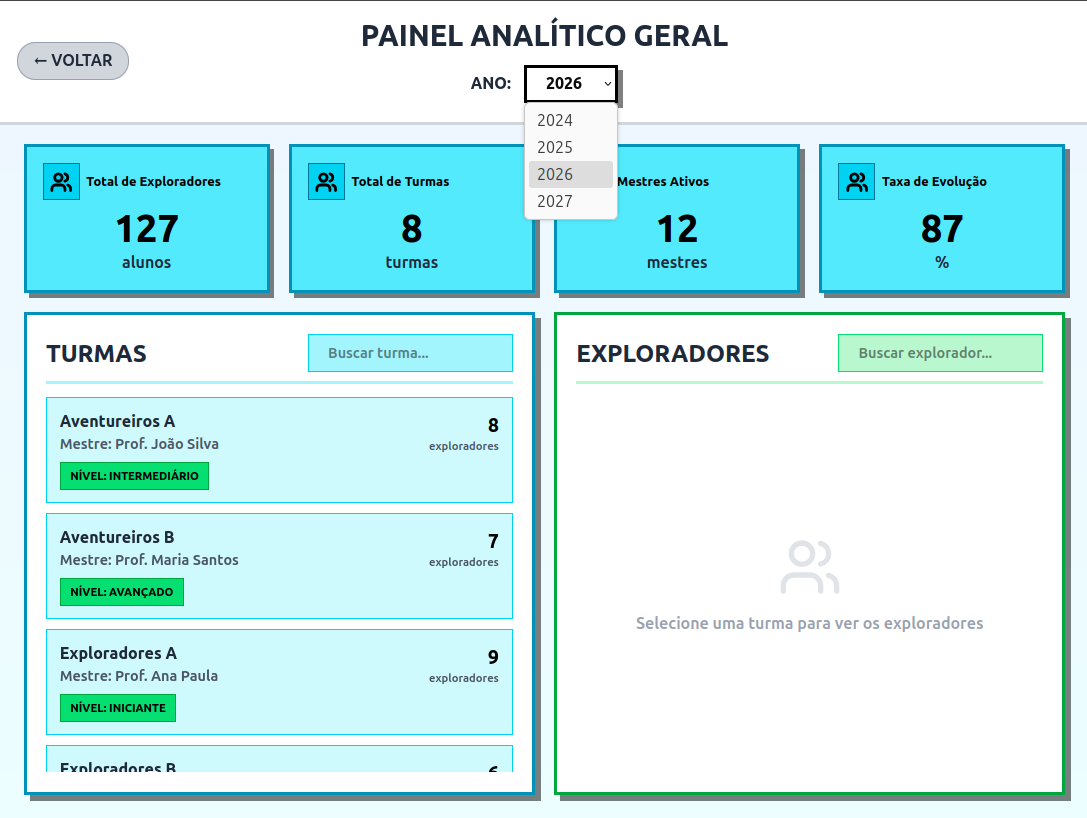
\includegraphics[width=0.85\textwidth]{adm40_painel_analitico3.png}
  \caption*{\small\textit{Fonte: Autoria própria, 2026.}}
\end{figure}
\textbf{Painel Analítico Geral (Visão do Guardião):} Esta interface fornece ao Guardião
uma visão macro do ecossistema pedagógico por meio de indicadores agregados (total de
exploradores, turmas, mestres ativos e taxa de evolução) e de dois painéis interativos de
navegação: a lista de Turmas à esquerda e a grade de Exploradores à direita, que se
popula dinamicamente ao selecionar uma turma. A funcionalidade de filtro por ano letivo
permite comparar a evolução institucional entre diferentes ciclos, enquanto o botão ``Ver
Mais Detalhes da Turma'' expande a análise para o nível individual de cada explorador,
tornando este painel o principal instrumento de tomada de decisão pedagógica da
plataforma.
 
% ============================================================
 
\section{DIAGRAMA DE CASOS DE USO}
% ============================================================
 
A modelagem de casos de uso foi organizada por atores e subsistemas, com o objetivo de
facilitar a compreensão das responsabilidades de cada perfil dentro da plataforma.
Os diagramas representam as interações entre os usuários e as funcionalidades
principais do sistema gamificado. A visão geral da organização é apresentada inicialmente
por meio de uma árvore hierárquica, seguida pelos diagramas UML detalhados de cada perfil
de usuário.
 
% ==============================================================
\subsection{Árvore de Organização do Modelo de Casos de Uso}
% ==============================================================
 
A árvore de organização do modelo de casos de uso apresenta a estrutura hierárquica
completa das funcionalidades do Sistema Gamificado de Atividades, organizada a partir de
três níveis principais: \textbf{Visão de Projeto}, \textbf{Visão de Casos de Uso} e
\textbf{Casos de Uso} por perfil de ator.
 
\begin{figure}[H]
    \centering
    \caption*{Árvore de Organização do Modelo de Casos de Uso.}
    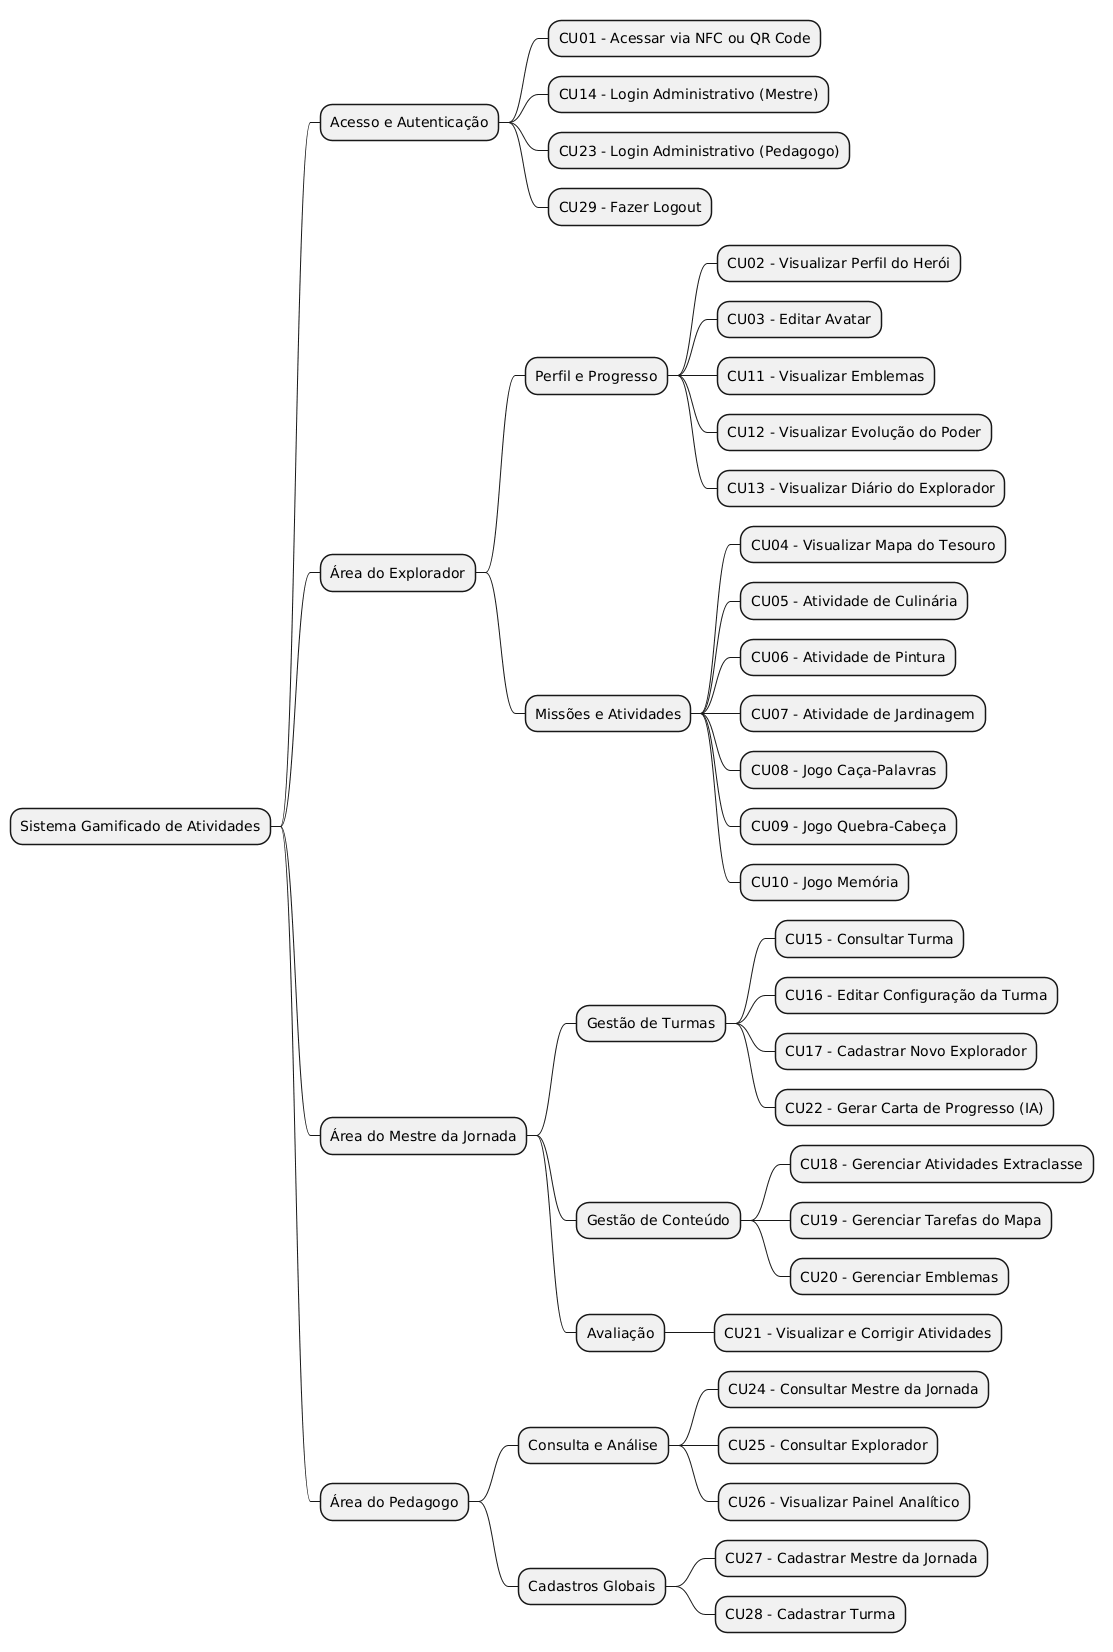
\includegraphics[width=0.95\textwidth]{arvore-cu.png}
    \caption*{\small\textit{Fonte: Adaptado de ChatGPT, 2026. Gerada via PlantUML.}}
\end{figure}
 
A raiz da árvore representa o \textbf{Sistema Gamificado de Atividades} e se ramifica
em duas visões complementares. A \textbf{Visão de Projeto} agrupa os três atores do
sistema --- Explorador (Aluno), Mestre da Jornada (Professor) e Pedagogo (Guardião) ---,
deixando explícita a separação de responsabilidades entre os perfis de acesso. A
\textbf{Visão de Casos de Uso} expande cada ator em seus respectivos agrupamentos
funcionais, distribuídos conforme a seguir.
 
O \textbf{Explorador} possui casos de uso organizados em três grupos: \textit{Acesso e
Autenticação} (CU01 e CU29), \textit{Perfil e Progresso} (CU02, CU03, CU11, CU12 e
CU13) e \textit{Missões e Atividades} (CU04 a CU10). Esses agrupamentos refletem as
três grandes jornadas do aluno na plataforma: entrar no sistema, acompanhar seu
desenvolvimento e executar as atividades pedagógicas gamificadas.
 
O \textbf{Mestre da Jornada} organiza seus casos de uso em quatro grupos:
\textit{Acesso e Autenticação} (CU14 e CU29), \textit{Gestão de Turmas} (CU15, CU16,
CU17 e CU22), \textit{Gestão de Conteúdo} (CU18, CU19 e CU20) e \textit{Avaliação}
(CU21). Essa estrutura evidencia a dupla responsabilidade do professor: gerenciar a
composição pedagógica das turmas e acompanhar o desempenho individual dos exploradores.
 
O \textbf{Pedagogo} concentra seus casos de uso em três grupos: \textit{Acesso e
Autenticação} (CU23 e CU29), \textit{Consulta e Análise} (CU24, CU25 e CU26) e
\textit{Cadastros Globais} (CU27 e CU28). Esse agrupamento traduz a atuação estratégica
do coordenador pedagógico, que atua predominantemente na supervisão institucional e na
configuração inicial da estrutura do sistema.
 
Vale destacar que o caso de uso \textbf{CU29 --- Fazer Logout} é compartilhado pelos
três perfis, aparecendo de forma recorrente na árvore dentro do grupo \textit{Acesso e
Autenticação} de cada ator. Essa repetição é intencional e reforça que o encerramento de
sessão é uma responsabilidade transversal, independente do nível de privilégio do usuário
autenticado.
 
\clearpage
\subsection{Perfil Explorador (Aluno)}
 
O ator ``Explorador'' representa o aluno que interage diretamente com as atividades
pedagógicas gamificadas da plataforma. Este perfil possui funcionalidades voltadas ao
acesso do sistema, visualização de progresso, personalização do avatar, execução de
atividades extraclasses e participação em minijogos educacionais.
 
As relações de dependência entre casos de uso foram modeladas utilizando os estereótipos
\textit{<<include>>} e \textit{<<extend>>}, permitindo representar reutilização de
funcionalidades e comportamentos opcionais dentro do fluxo principal de interação.
 
\begin{figure}[H]
    \centering
    \caption*{Diagrama de Casos de Uso --- Perfil Explorador (Aluno).}
    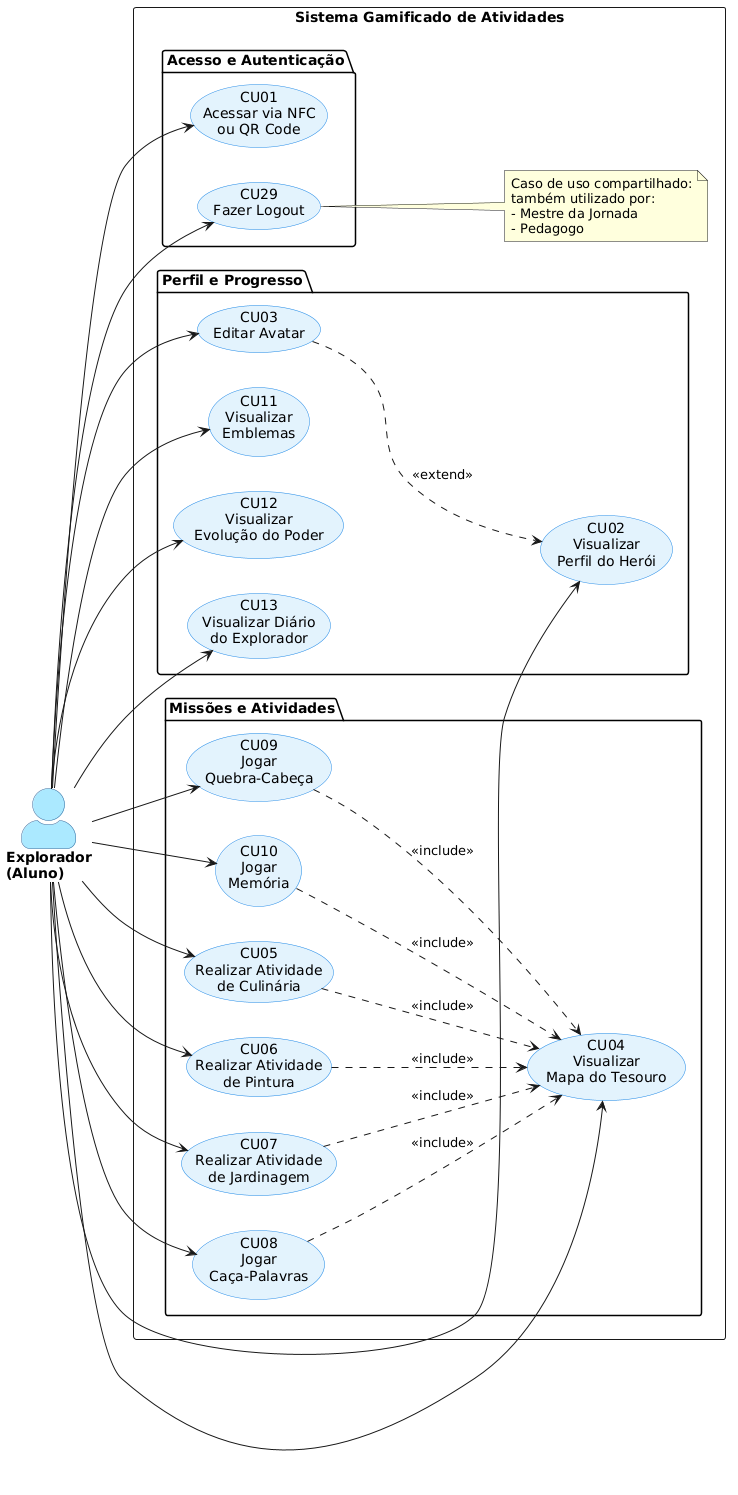
\includegraphics[width=0.65\textwidth]{cu-explorador.png}
    \caption*{\small\textit{Fonte: Adaptado de Claude (Anthropic), 2026. Gerado via PlantUML.}}
\end{figure}
 
\textbf{Descrição Geral dos Casos de Uso do Explorador:}
 
\begin{itemize}
    \item \textbf{CU01 --- Acessar via NFC ou QR Code:} Permite ao explorador realizar autenticação simplificada no sistema.
 
    \item \textbf{CU02 --- Visualizar Perfil do Herói:} Exibe informações gerais do explorador, incluindo progresso, avatar, evolução e estatísticas.
 
    \item \textbf{CU03 --- Editar Avatar:} Permite personalizar a aparência visual do personagem do explorador.
 
    \item \textbf{CU04 --- Visualizar Mapa do Tesouro:} Exibe o mapa principal contendo missões, atividades e progresso desbloqueado.
 
    \item \textbf{CU05 --- Realizar Atividade de Culinária:} Executa desafios pedagógicos relacionados ao módulo de culinária.
 
    \item \textbf{CU06 --- Realizar Atividade de Pintura:} Executa atividades criativas relacionadas ao módulo de pintura.
 
    \item \textbf{CU07 --- Realizar Atividade de Jardinagem:} Executa tarefas interativas ligadas ao módulo de jardinagem.
 
    \item \textbf{CU08 --- Jogar Caça-Palavras:} Disponibiliza minijogos educativos de associação textual.
 
    \item \textbf{CU09 --- Jogar Quebra-Cabeça:} Disponibiliza desafios lógicos e visuais baseados em montagem de imagens.
 
    \item \textbf{CU10 --- Jogar Memória:} Disponibiliza atividades de memória e associação visual.
 
    \item \textbf{CU11 --- Visualizar Emblemas:} Permite consultar recompensas, medalhas e conquistas obtidas.
 
    \item \textbf{CU12 --- Visualizar Evolução do Poder:} Exibe métricas de desenvolvimento e evolução do explorador.
 
    \item \textbf{CU13 --- Visualizar Diário do Explorador:} Exibe registros históricos das atividades realizadas e progresso acumulado.
 
    \item \textbf{CU29 --- Fazer Logout:} Finaliza a sessão do usuário na plataforma.
\end{itemize}
 
 
\newpage
\subsection{Perfil Mestre da Jornada (Professor)}
 
O ator ``Mestre da Jornada'' representa o professor responsável pelo gerenciamento
pedagógico das turmas, acompanhamento dos exploradores e administração das atividades
educacionais disponibilizadas na plataforma.
 
Este perfil possui funcionalidades relacionadas à organização das turmas, criação e
gerenciamento de conteúdos extraclasses, correção de atividades e acompanhamento do
desenvolvimento dos alunos por meio de relatórios e cartas de progresso.
 
\begin{figure}[H]
    \centering
    \caption*{Diagrama de Casos de Uso --- Perfil Mestre da Jornada (Professor).}
    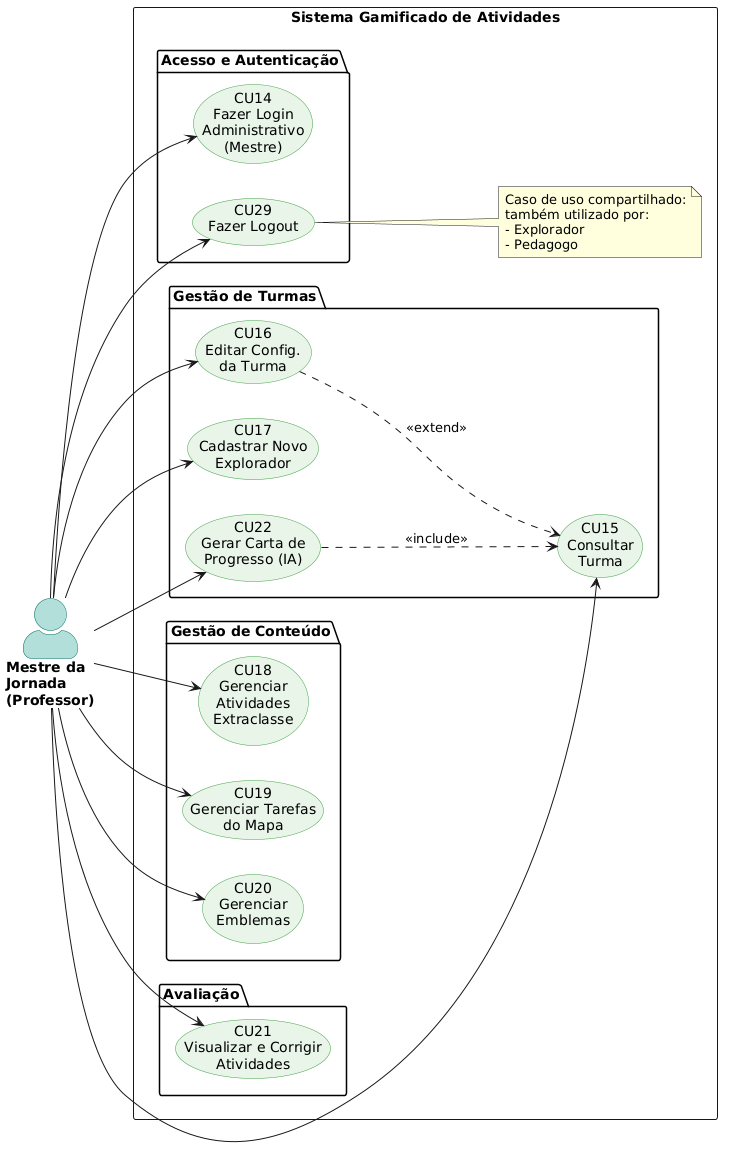
\includegraphics[width=0.85\textwidth]{cu-mestredajornada.png}
    \caption*{\small\textit{Fonte: Adaptado de Claude (Anthropic), 2026. Gerado via PlantUML.}}
\end{figure}
 
\textbf{Descrição Geral dos Casos de Uso do Mestre da Jornada:}
 
\begin{itemize}
    \item \textbf{CU14 --- Fazer Login Administrativo (Mestre):} Permite autenticação administrativa do professor no sistema.
 
    \item \textbf{CU15 --- Consultar Turma:} Exibe informações gerais da turma, alunos cadastrados e progresso coletivo.
 
    \item \textbf{CU16 --- Editar Configuração da Turma:} Permite alterar informações e parâmetros da turma.
 
    \item \textbf{CU17 --- Cadastrar Novo Explorador:} Permite registrar novos alunos vinculados à turma.
 
    \item \textbf{CU18 --- Gerenciar Atividades Extraclasse:} Permite criar, editar e remover atividades pedagógicas.
 
    \item \textbf{CU19 --- Gerenciar Tarefas do Mapa:} Permite configurar desafios e missões presentes no mapa gamificado.
 
    \item \textbf{CU20 --- Gerenciar Emblemas:} Permite administrar recompensas e medalhas distribuídas aos exploradores.
 
    \item \textbf{CU21 --- Visualizar e Corrigir Atividades:} Permite acompanhar respostas e avaliar atividades realizadas pelos alunos.
 
    \item \textbf{CU22 --- Gerar Carta de Progresso (IA):} Gera automaticamente relatórios descritivos de desempenho dos alunos utilizando inteligência artificial.
 
    \item \textbf{CU29 --- Fazer Logout:} Finaliza a sessão do usuário na plataforma.
\end{itemize}
 
\newpage
\subsection{Perfil Pedagogo (Guardião)}
 
O ator ``Pedagogo'' representa o responsável administrativo e analítico da plataforma.
Este perfil possui permissões voltadas à supervisão institucional, gerenciamento global
de usuários e acompanhamento estratégico do ambiente educacional.
 
As funcionalidades disponibilizadas ao pedagogo permitem análise de desempenho,
cadastro de professores e turmas, além da visualização de indicadores analíticos do sistema.
 
\begin{figure}[H]
    \centering
    \caption*{Diagrama de Casos de Uso --- Perfil Pedagogo (Guardião).}
    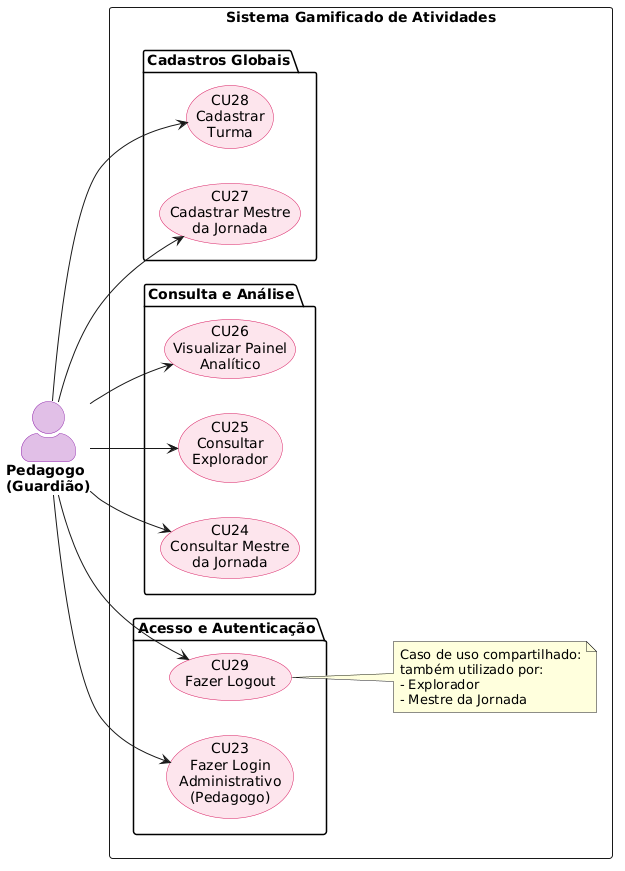
\includegraphics[width=0.85\textwidth]{cu-pedagogo.png}
    \caption*{\small\textit{Fonte: Adaptado de Claude (Anthropic), 2026. Gerado via PlantUML.}}
\end{figure}
 
\textbf{Descrição Geral dos Casos de Uso do Pedagogo:}
 
\begin{itemize}
    \item \textbf{CU23 --- Fazer Login Administrativo (Pedagogo):} Permite autenticação administrativa do pedagogo no sistema.
 
    \item \textbf{CU24 --- Consultar Mestre da Jornada:} Permite visualizar informações e desempenho dos professores cadastrados.
 
    \item \textbf{CU25 --- Consultar Explorador:} Permite acompanhar dados individuais dos alunos cadastrados.
 
    \item \textbf{CU26 --- Visualizar Painel Analítico:} Exibe métricas, estatísticas e indicadores gerais do sistema.
 
    \item \textbf{CU27 --- Cadastrar Mestre da Jornada:} Permite registrar novos professores na plataforma.
 
    \item \textbf{CU28 --- Cadastrar Turma:} Permite criar e organizar novas turmas dentro do sistema.
 
    \item \textbf{CU29 --- Fazer Logout:} Finaliza a sessão do usuário na plataforma.
\end{itemize}
 
 
\section{DIAGRAMA DE CLASSES}
 
O Diagrama de Classes representa a estrutura estática do sistema, 
definindo as classes que o compõem, seus atributos, métodos e os 
relacionamentos entre elas. Para o Sistema Gamificado de Atividades, 
o diagrama foi organizado em seis grupos principais: hierarquia de 
usuários, identidade e acesso, turmas e habilidades, missões e 
atividades, emblemas e relatórios.
 
\subsection{Hierarquia de Usuários}
 
A classe abstrata \textit{Usuario} serve como base para os três 
perfis do sistema: \textit{Explorador} (aluno), 
\textit{MestreJornada} (professor) e \textit{Pedagogo}. Essa 
estrutura de herança centraliza os atributos comuns de autenticação 
— nome, e-mail e senha — evitando redundância e facilitando a 
manutenção do sistema.
 
O \textit{Explorador} concentra as operações relacionadas à jornada 
do aluno, como visualizar o perfil, o Mapa do Tesouro, os emblemas 
conquistados e o Diário do Explorador. O \textit{MestreJornada} 
agrupa as responsabilidades de gestão, incluindo o cadastro de 
exploradores, o gerenciamento de atividades, a correção de missões, 
a geração de cartas de progresso e o cadastro de emblemas. Já o 
\textit{Pedagogo} possui acesso ao painel analítico do sistema.
 
\subsection{Identidade, Acesso e Personalização}
 
Cada \textit{Explorador} possui uma \textit{IdentidadeDigital} única, 
que pode ser do tipo NFC ou QR Code, utilizada para validar o acesso 
ao sistema de forma autônoma. A classe \textit{Avatar} permite a 
personalização da representação visual do aluno. Caso o explorador 
possua alguma necessidade especial, a classe \textit{EquipamentoApoio} 
define o recurso de acessibilidade adequado, como feedback por áudio 
ou interface em alto contraste.
 
\subsection{Turmas e Habilidades}
 
A classe \textit{Turma} organiza grupos de até dez exploradores, 
vinculados a um \textit{MestreJornada} responsável. Cada explorador 
possui seis instâncias de \textit{PoderHabilidade}, representando 
competências como criatividade, coordenação motora e raciocínio 
lógico, cada uma com seu próprio nível de evolução — definido pelo 
enumerador \textit{NivelEvolucao}, que vai de ``Em Treinamento'' 
até ``Mestre''.
 
\subsection{Missões e Atividades}
 
As atividades do sistema são organizadas por meio do 
\textit{MapaTesouro}, que agrega as \textit{Missoes} disponíveis 
para o explorador. Cada missão possui um status — bloqueado, ativo 
ou completo — e está associada a uma implementação concreta da 
classe abstrata \textit{Atividade}.
 
Foram modeladas seis subclasses de atividade: 
\textit{AtividadeCulinaria}, \textit{AtividadePintura}, 
\textit{AtividadeJardinagem}, \textit{JogoCacaPalavras}, 
\textit{JogoQuebracabeca} e \textit{JogoMemoria}. Cada uma 
sobrescreve o método \texttt{calcularNota()} com sua própria 
lógica de avaliação. Os resultados são registrados pela classe 
\textit{ResultadoAtividade}, que armazena tanto a nota calculada 
automaticamente quanto a nota final, que pode ser editada pelo 
\textit{MestreJornada}.
 
\subsection{Emblemas e Relatórios}
 
Os emblemas conquistados pelo explorador são representados pela 
classe \textit{Emblema}, organizada por categorias como Explorador, 
Criador e Mestre. Novos emblemas podem ser criados pelo 
\textit{MestreJornada} conforme a necessidade pedagógica.
 
Por fim, o sistema conta com três mecanismos de acompanhamento: 
o \textit{DiarioExplorador}, que registra a linha do tempo de 
conquistas do aluno; a \textit{CartaProgresso}, gerada com apoio 
de Inteligência Artificial e enviada aos responsáveis; e o 
\textit{PainelAnalitico}, disponível ao \textit{Pedagogo} para 
acompanhar a evolução das turmas por diferentes ciclos.
 
\begin{figure}[H]
    \centering
    \caption{Diagrama de Classes do Sistema Gamificado de Atividades}
    \label{fig:diagrama_classes}
    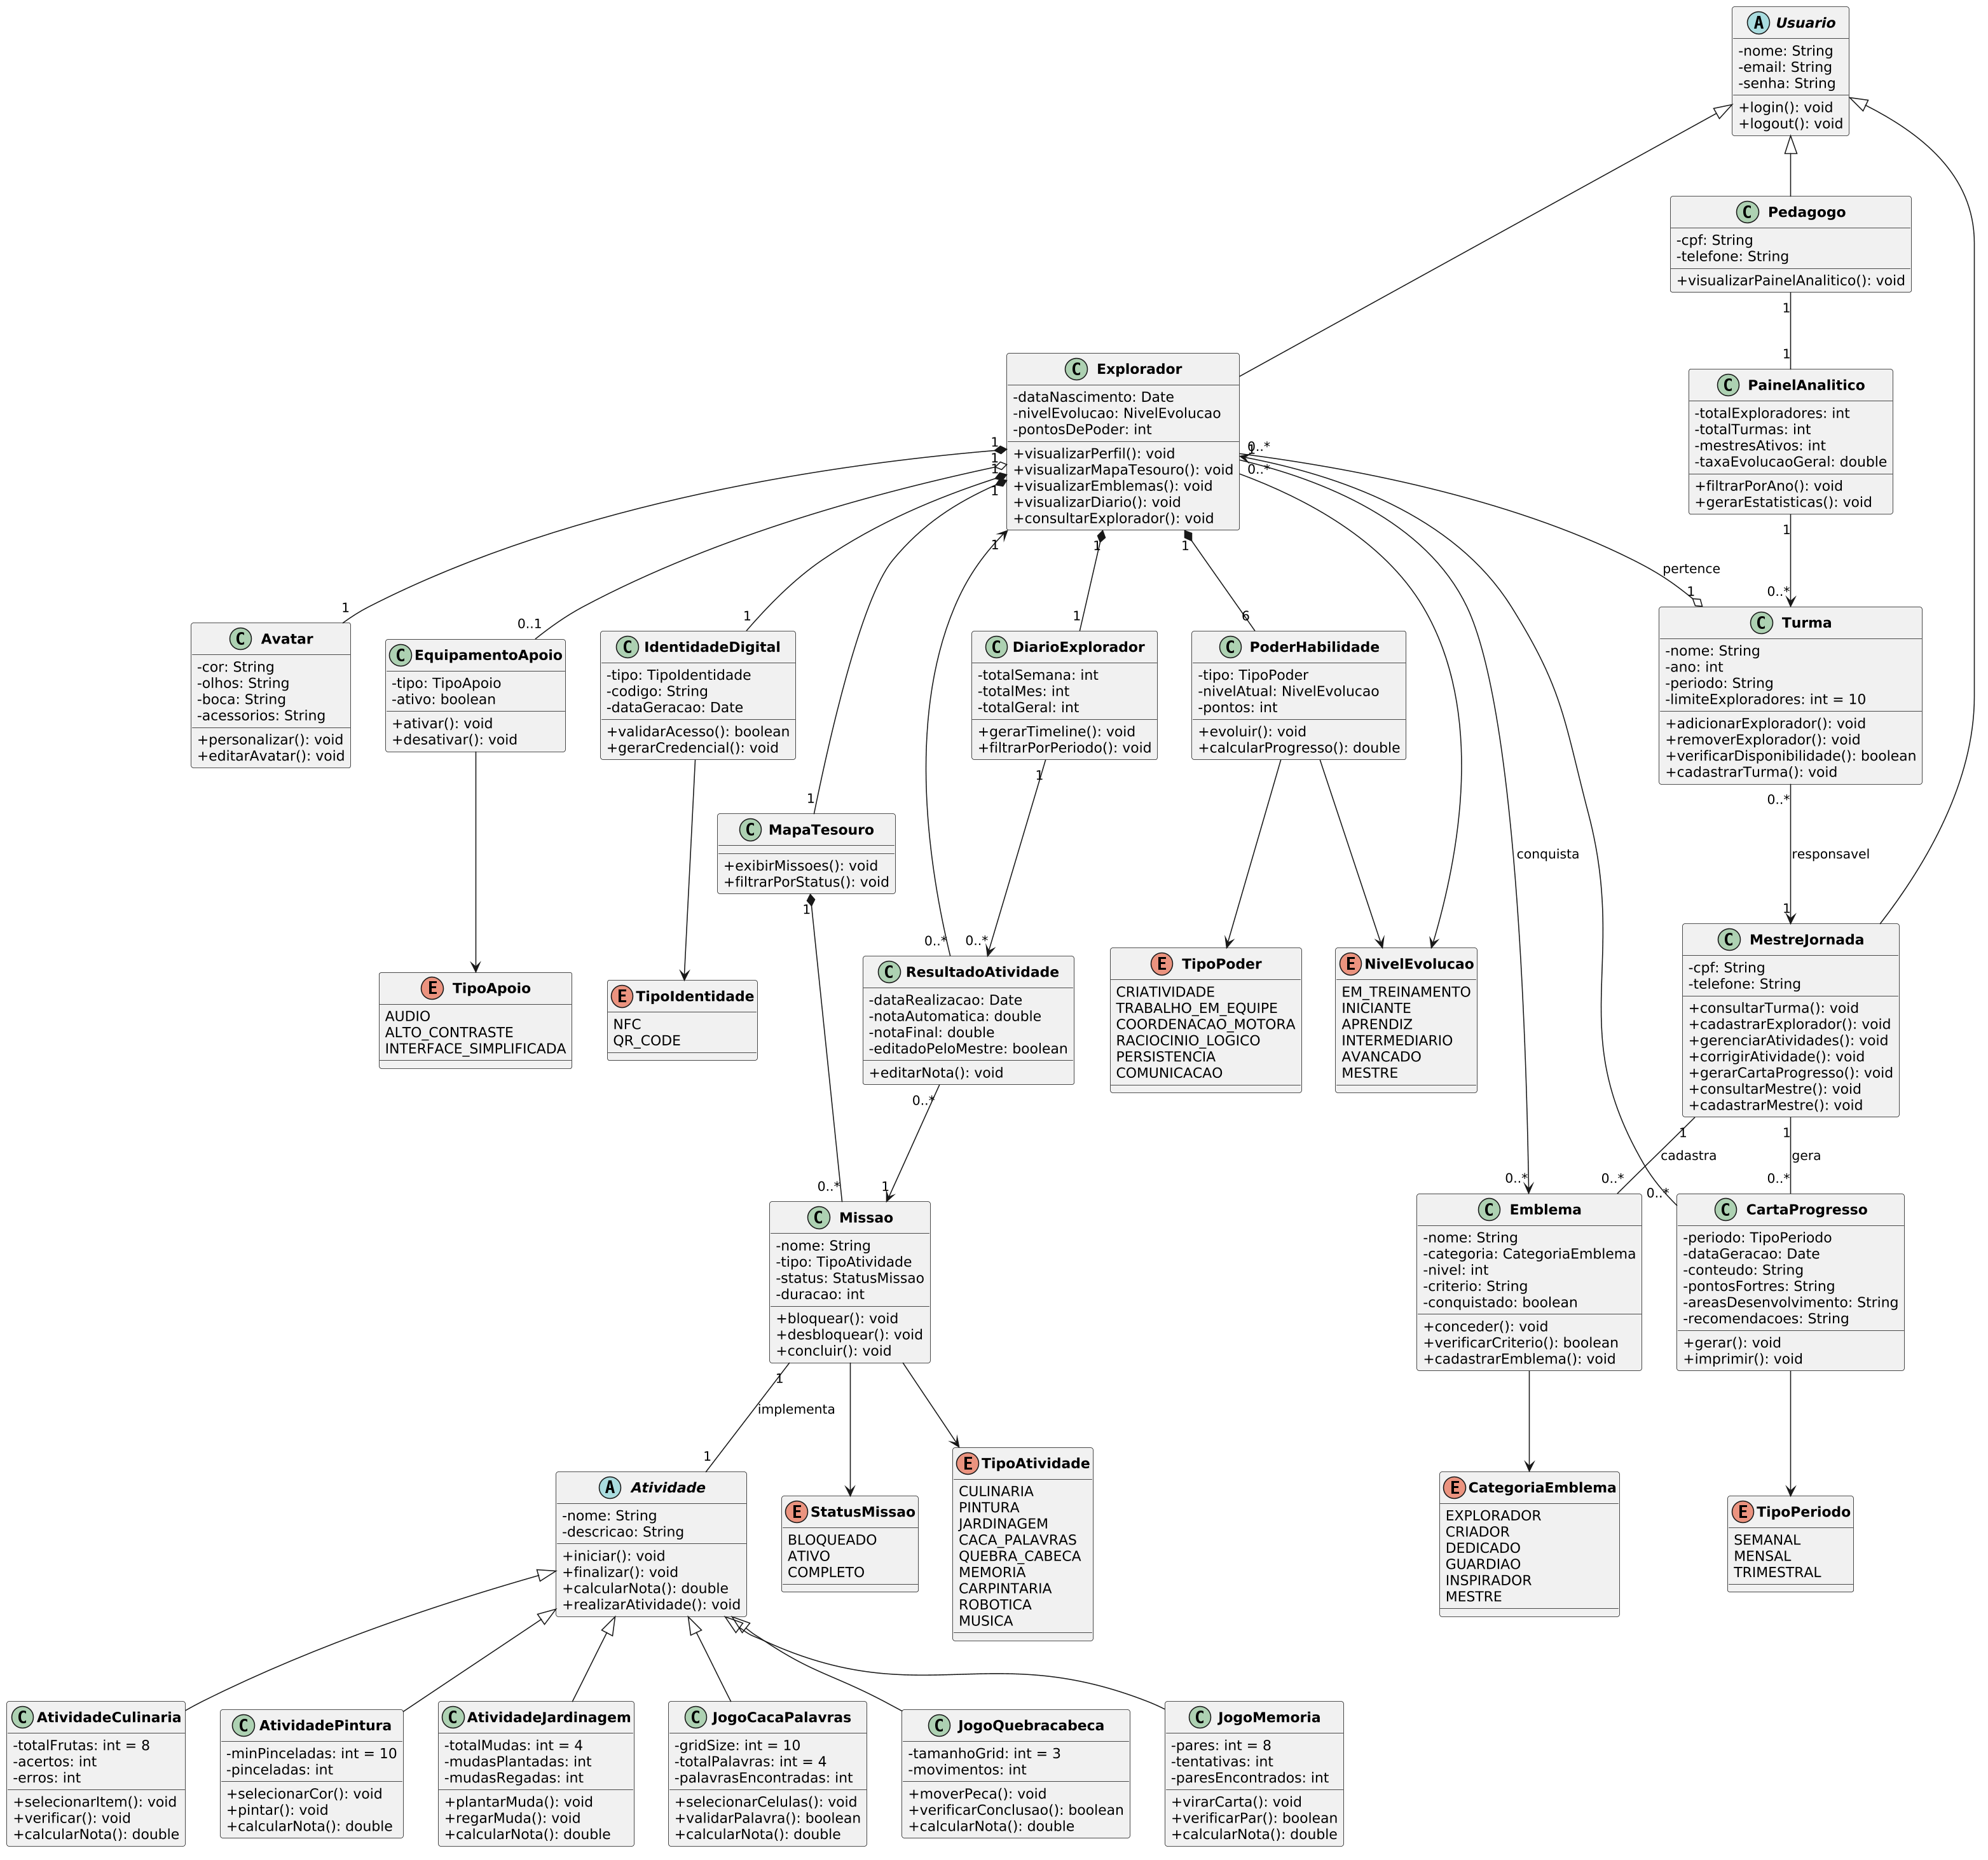
\includegraphics[width=\textwidth]{figuras/image.png}
\end{figure}
 
\clearpage
 
\section{DIAGRAMAS DE SEQUÊNCIA}
 
Os Diagramas de Sequência representam a interação entre os objetos
do sistema ao longo do tempo, evidenciando a troca de mensagens
entre os participantes para a realização de cada funcionalidade.
Foram elaborados três diagramas, escolhidos de forma a cobrir
fluxos distintos entre si: autenticação via hardware, gerenciamento
administrativo e personalização do perfil do aluno.
 
\subsection{Login do Explorador via NFC/QR Code}
 
O diagrama da Figura~\ref{fig:seq_login} representa o fluxo de
autenticação do Explorador por meio de pulseira NFC ou QR Code.
O processo tem início quando o aluno aproxima a pulseira do
dispositivo (tablet ou totem), que captura o código e o encaminha
ao sistema. A classe \textit{IdentidadeDigital} é consultada para
validar a credencial. Em caso de sucesso, o sistema inicia a sessão
e carrega o Mural do Explorador. Caso a identidade não seja
encontrada, o acesso é negado e uma mensagem de erro é exibida ao
aluno. Este fluxo garante a autonomia de crianças em fase de
alfabetização ou com deficiência intelectual, dispensando o uso
de senhas.
 
\begin{figure}[H]
    \centering
    \caption{Diagrama de Sequência – Login do Explorador via NFC/QR Code}
    \label{fig:seq_login}
    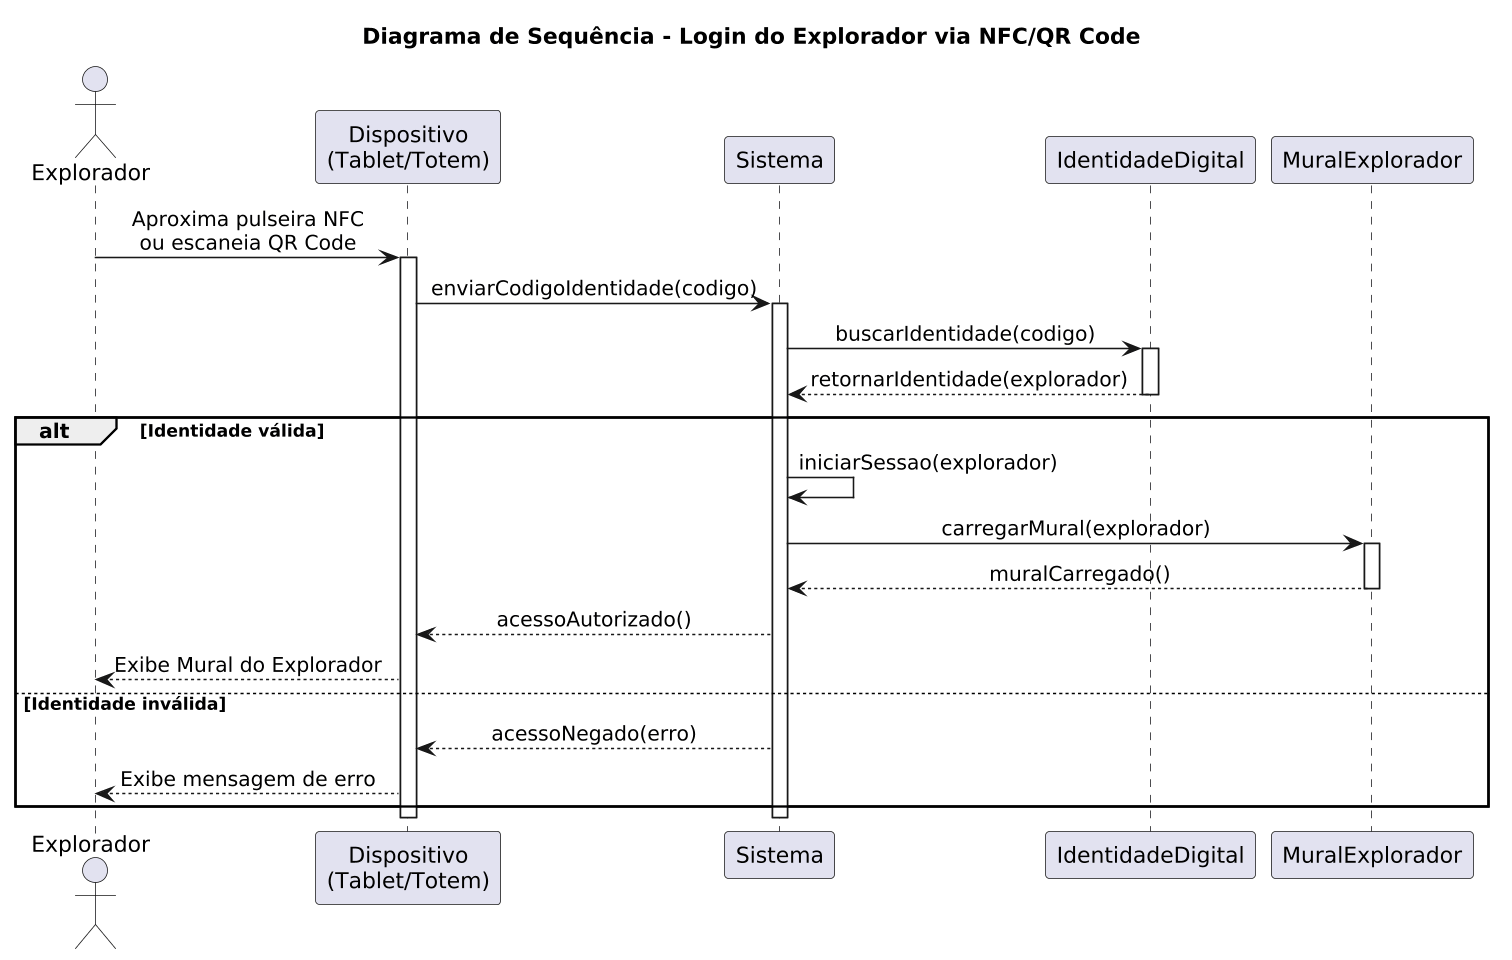
\includegraphics[width=\textwidth]{figuras/seq1_login.png}
\end{figure}
 
\subsection{Cadastrar Turma}
 
O diagrama da Figura~\ref{fig:seq_turma} ilustra o fluxo de
cadastro de uma nova turma pelo Pedagogo. Após acessar o menu
de cadastro e preencher os dados da turma — nome, ano letivo e
período —, o sistema verifica a disponibilidade do Mestre da
Jornada selecionado. Caso o Mestre esteja disponível, a classe
\textit{Turma} é instanciada com limite padrão de dez exploradores
e o cadastro é concluído com sucesso. No fluxo alternativo, caso
não haja nenhum Mestre cadastrado no sistema, o Pedagogo é
redirecionado para a tela de cadastro de Mestre antes de
prosseguir.
 
\begin{figure}[H]
    \centering
    \caption{Diagrama de Sequência – Cadastrar Turma}
    \label{fig:seq_turma}
    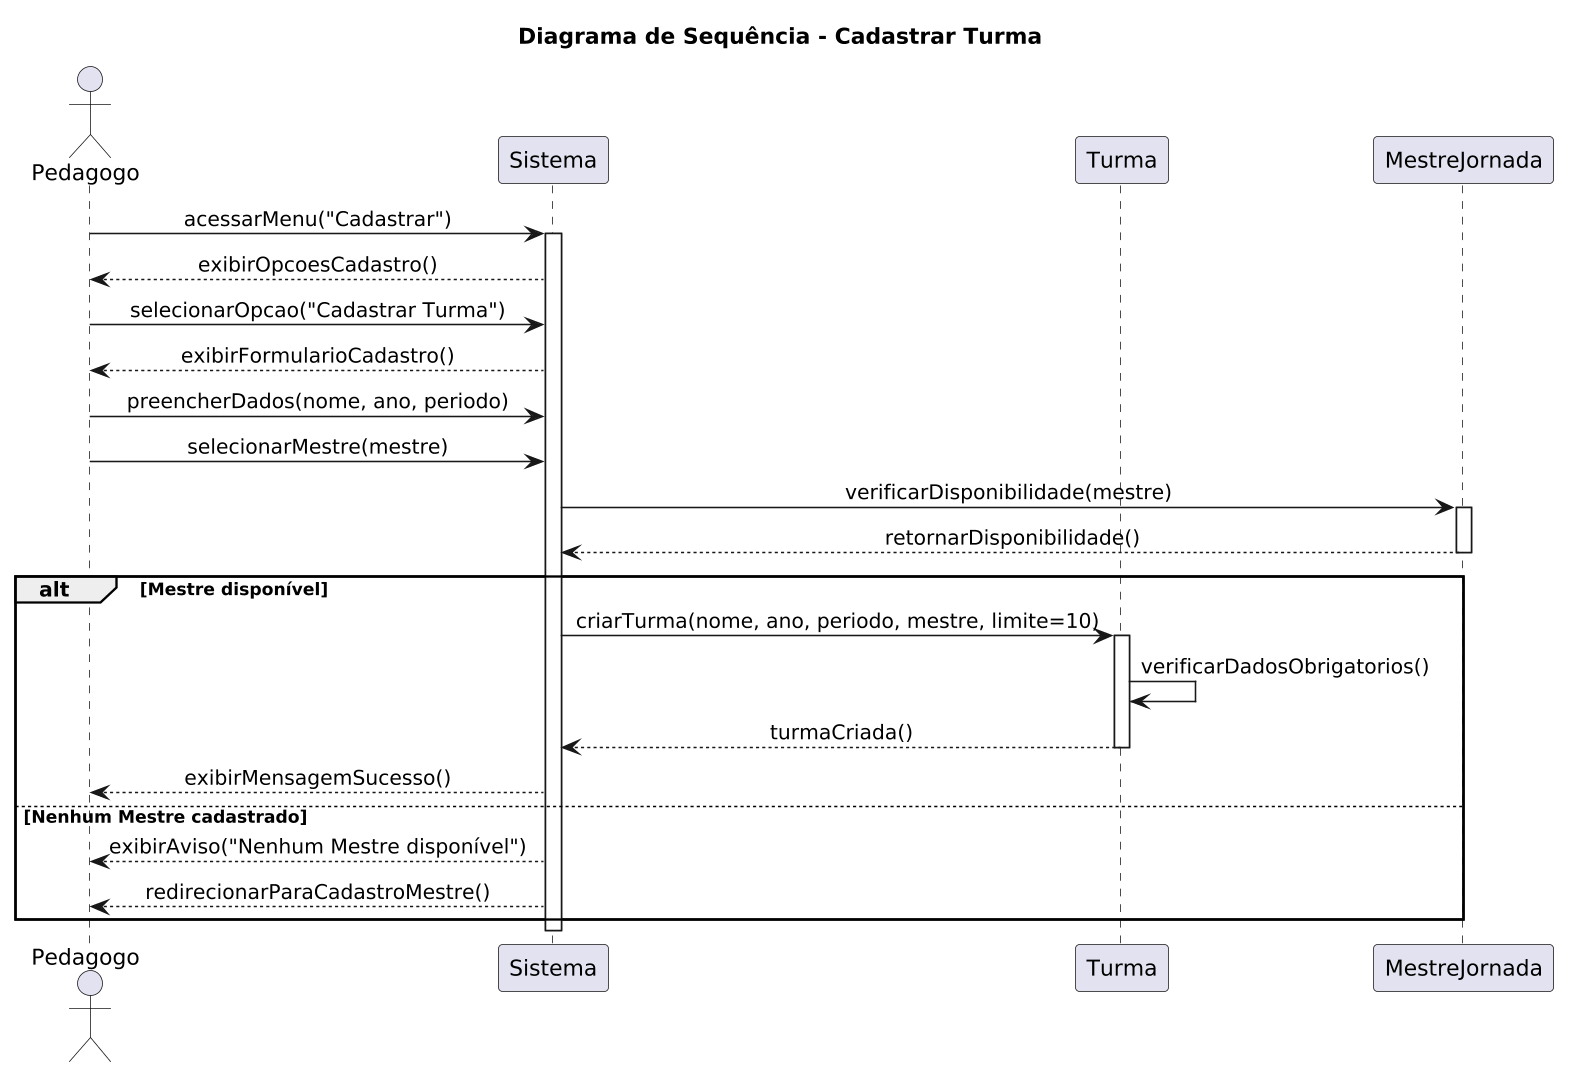
\includegraphics[width=\textwidth]{figuras/seq2_cadas_turma.png}
\end{figure}
 
\subsection{Alterar Avatar}
 
O diagrama da Figura~\ref{fig:seq_avatar} descreve o fluxo de
personalização do avatar pelo Explorador. A partir do Perfil do
Herói, o aluno acessa a tela de personalização, onde a classe
\textit{Avatar} carrega as opções disponíveis de cor, olhos, boca
e acessórios. Um laço de repetição permite que o Explorador
selecione e visualize o preview de cada alteração antes de
confirmar. Ao confirmar, o novo avatar é persistido pelo sistema
e o perfil é atualizado imediatamente, refletindo as escolhas do
aluno em toda a interface.
 
\begin{figure}[H]
    \centering
    \caption{Diagrama de Sequência – Alterar Avatar}
    \label{fig:seq_avatar}
    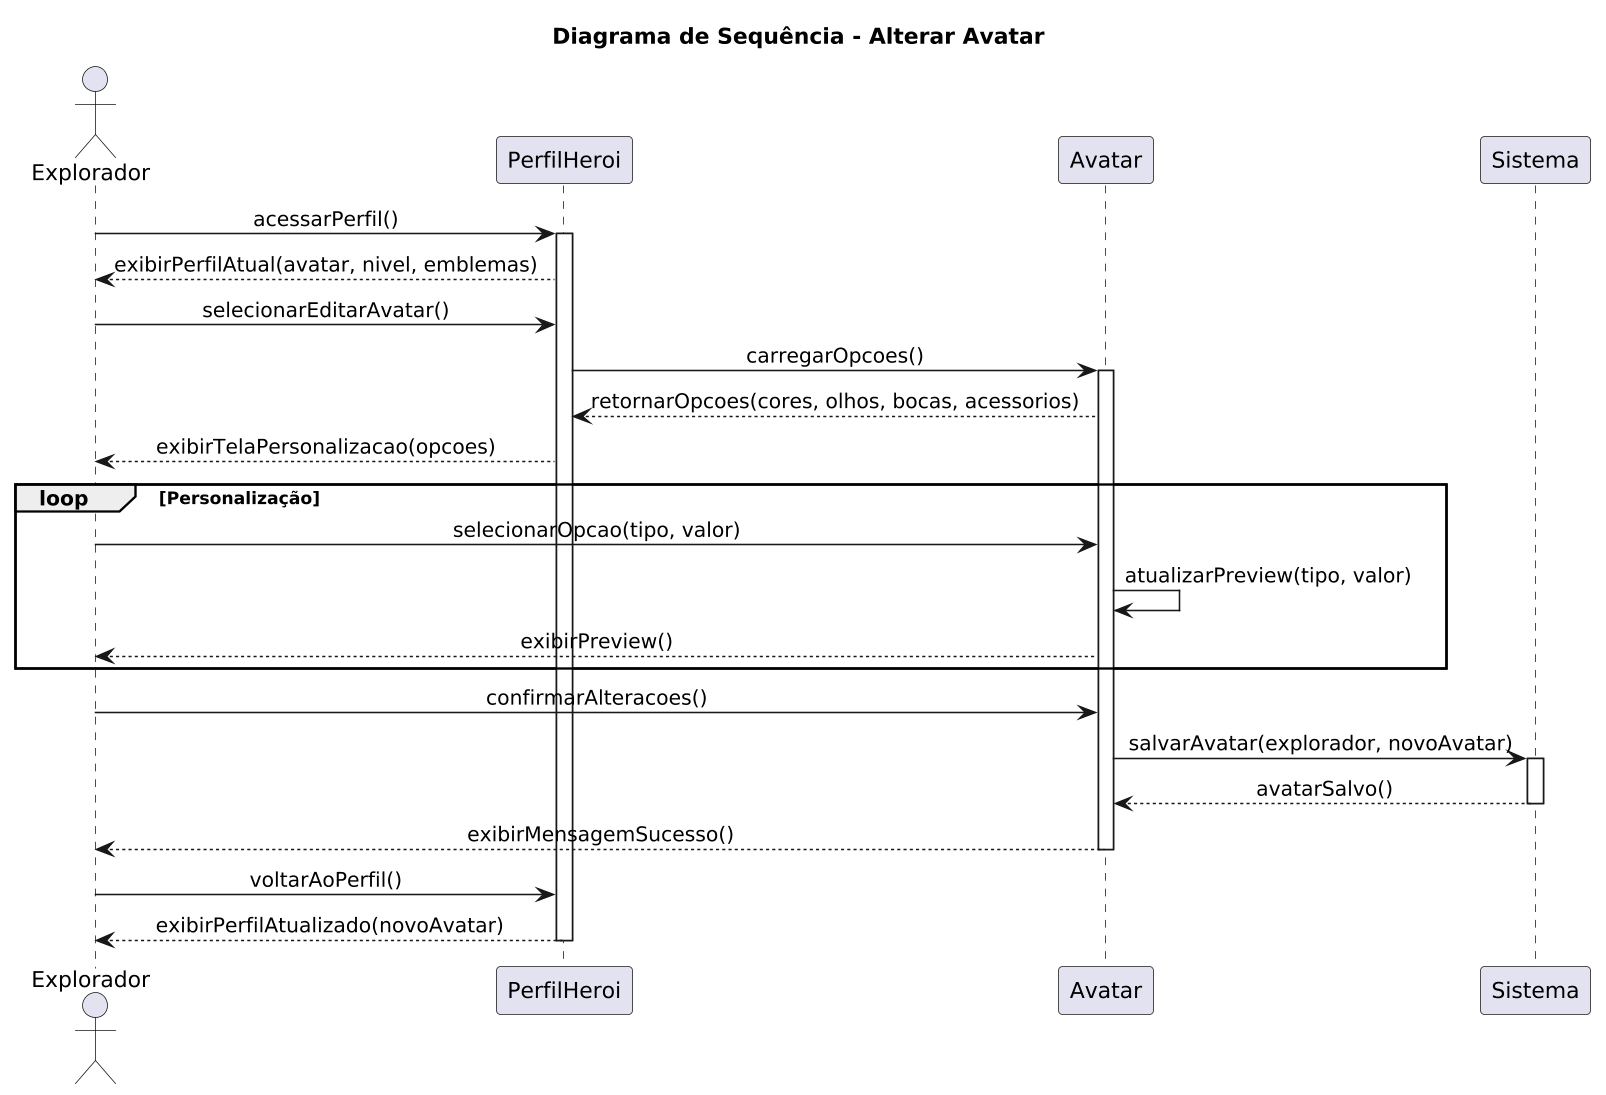
\includegraphics[width=\textwidth]{figuras/seq3_avatar.png}
\end{figure}
 
\section{DIAGRAMA DE COMUNICAÇÃO}
 
O Diagrama de Comunicação, também denominado Diagrama de
Colaboração na UML 1.x, representa as interações entre objetos
com foco nos vínculos estruturais entre eles, em contraste ao
Diagrama de Sequência, que enfatiza a ordem temporal das
mensagens. As mensagens são numeradas sequencialmente para
indicar a ordem de execução do fluxo.
 
O diagrama da Figura~\ref{fig:com_turma} foi elaborado com base
no fluxo de cadastro de turma, correspondente ao Diagrama de
Sequência apresentado na Seção~\ref{sec:seq_turma}. Os quatro
objetos envolvidos são \textit{Pedagogo}, \textit{Sistema},
\textit{MestreJornada} e \textit{Turma}. O \textit{Pedagogo}
inicia o fluxo acessando o menu de cadastro e preenchendo os
dados da turma (mensagens 1 a 6). O \textit{Sistema} então
consulta o \textit{MestreJornada} para verificar sua
disponibilidade (mensagens 7 e 8). Confirmada a disponibilidade,
o \textit{Sistema} aciona a criação da turma, que realiza a
validação interna dos dados obrigatórios antes de confirmar
o cadastro (mensagens 9 a 11). Por fim, o \textit{Sistema}
retorna a mensagem de sucesso ao \textit{Pedagogo} (mensagem 12).
 
\begin{figure}[H]
    \centering
    \caption{Diagrama de Comunicação – Cadastrar Turma}
    \label{fig:com_turma}
    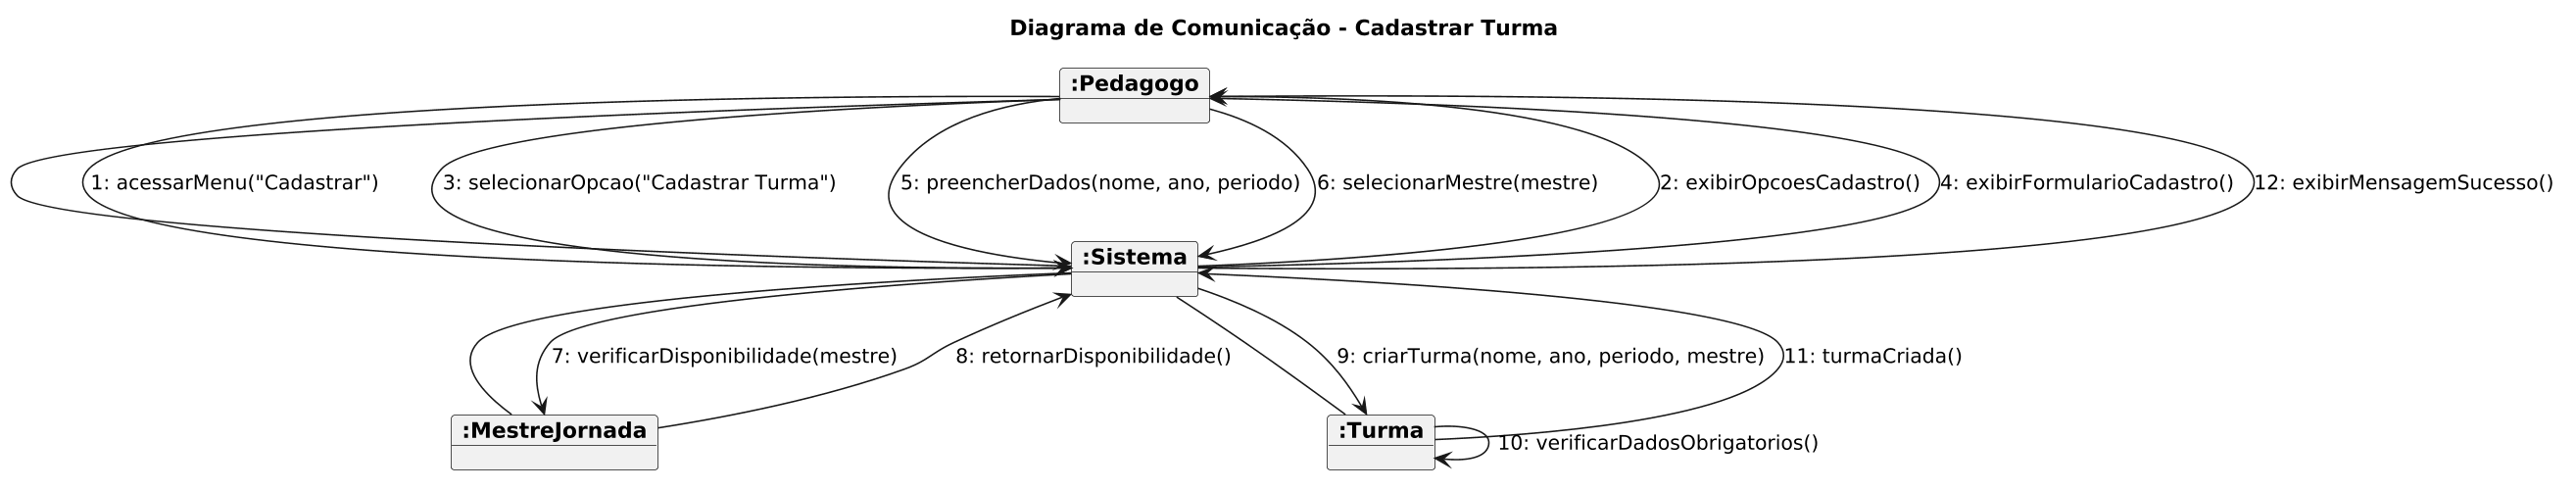
\includegraphics[width=\textwidth]{figuras/com_turma.png}
\end{figure}
 
\section{DIAGRAMAS DE ATIVIDADES}
 
O Diagrama de Atividades descreve o fluxo de controle entre
atividades de um processo, permitindo representar decisões,
paralelismos e responsabilidades de forma visual. Foram elaborados
dois diagramas, posicionados em visões distintas conforme a
natureza do elemento modelado.
 
\subsection{Operação calcularNota() — Classe JogoMemoria
            \texorpdfstring{\\}{}
            \normalfont\small[Visão de Projeto]}
 
O diagrama da Figura~\ref{fig:atv_nota} representa a lógica
interna da operação \texttt{calcularNota()} pertencente à classe
\textit{JogoMemoria}, sendo posicionado na \textbf{Visão de
Projeto} por modelar o comportamento interno de uma operação
de uma classe do sistema.
 
A operação recebe como entrada o número de tentativas realizadas
e a quantidade de pares encontrados. Caso o jogo não tenha sido
concluído, retorna nota zero. Quando concluído, calcula as
tentativas excedentes em relação ao mínimo esperado de oito,
aplicando uma penalidade de três pontos por tentativa adicional.
O resultado é limitado ao mínimo de 50 pontos, garantindo que
o Explorador sempre receba um retorno positivo pelo esforço.
 
\begin{figure}[H]
    \centering
    \caption{Diagrama de Atividades – Operação calcularNota() [Visão de Projeto]}
    \label{fig:atv_nota}
    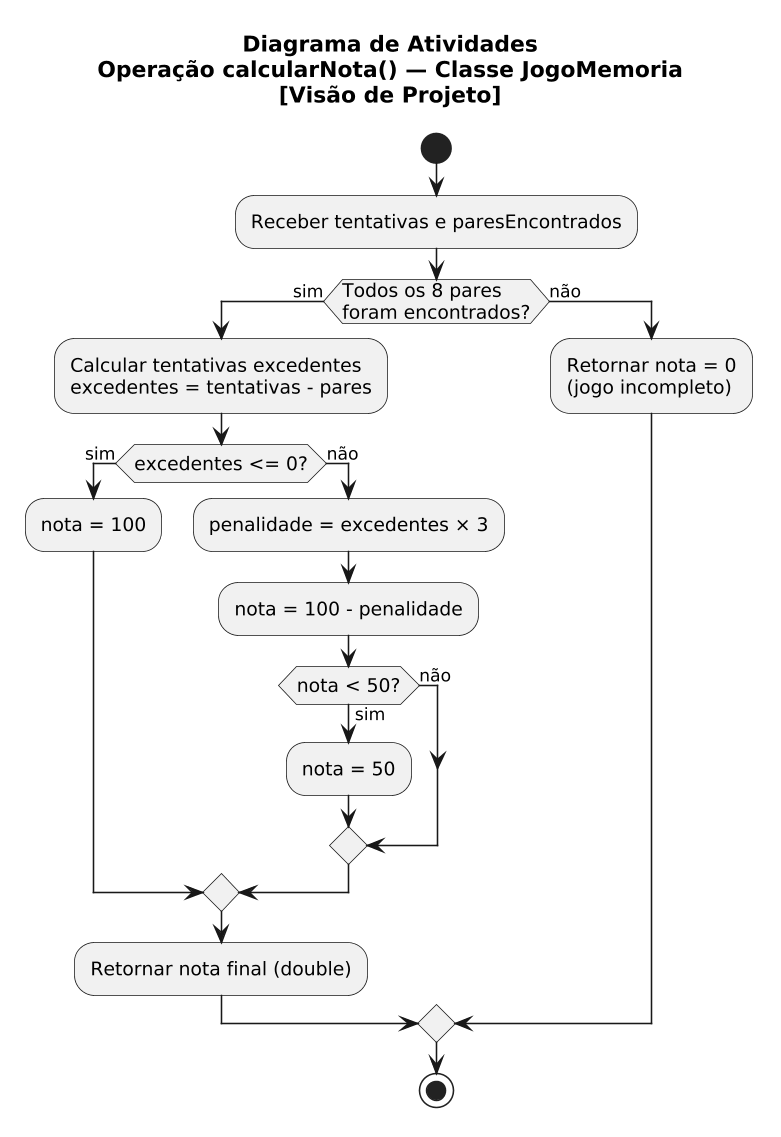
\includegraphics[width=0.65\textwidth]{figuras/atv1_calcularNota.png}
\end{figure}
 
\subsection{Caso de Uso: Cadastrar Explorador
            \texorpdfstring{\\}{}
            \normalfont\small[Visão de Casos de Uso]}
 
O diagrama da Figura~\ref{fig:atv_explorador} modela o fluxo
do caso de uso ``Cadastrar Explorador'', sendo posicionado na
\textbf{Visão de Casos de Uso} por representar uma funcionalidade
do sistema sob a perspectiva dos atores envolvidos.
 
O diagrama utiliza raias (\textit{swimlanes}) para separar as
responsabilidades do \textit{Mestre da Jornada} e do
\textit{Sistema}. O fluxo inicia com o preenchimento dos dados
do aluno e a seleção da turma. O sistema verifica a
disponibilidade de vagas; caso a turma esteja lotada, o Mestre
é orientado a selecionar outra. Havendo vaga, o Mestre escolhe
o tipo de identificação — NFC ou QR Code —, e o sistema registra
a credencial correspondente. Em seguida, o sistema verifica
automaticamente a necessidade de configurar um
\textit{EquipamentoApoio}, cria o Perfil do Herói com avatar
padrão e envia a credencial ao responsável por e-mail.
 
\begin{figure}[H]
    \centering
    \caption{Diagrama de Atividades – Cadastrar Explorador [Visão de Casos de Uso]}
    \label{fig:atv_explorador}
    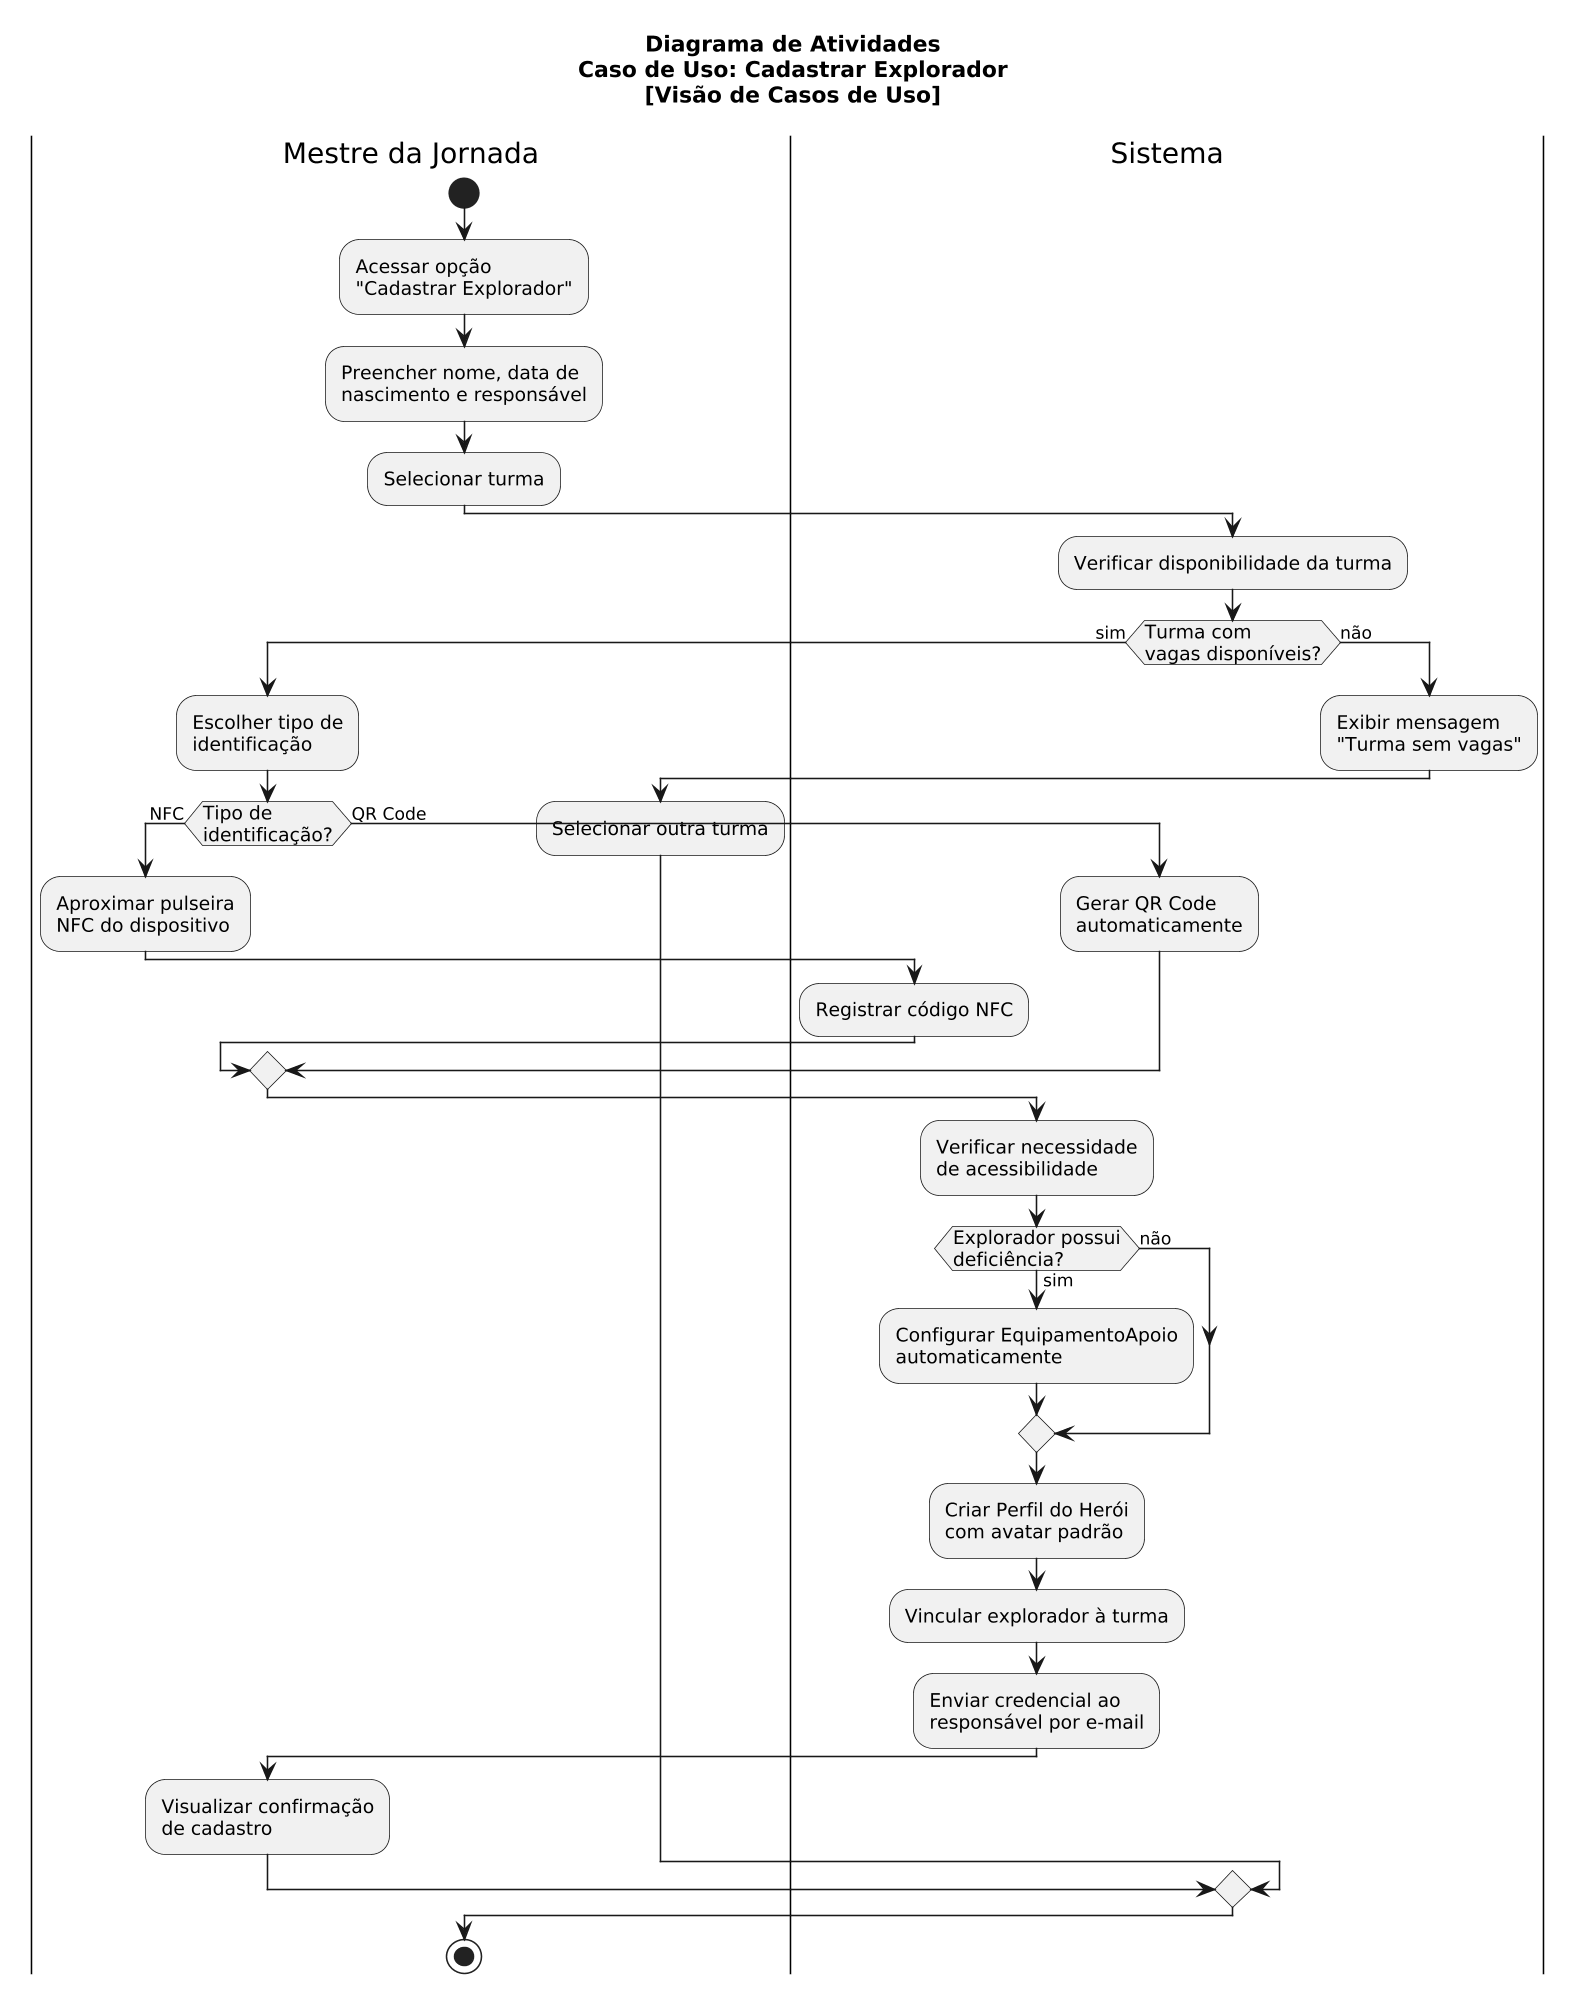
\includegraphics[width=\textwidth]{figuras/atv2_cadastrarExplorador.png}
\end{figure}
 
\section{DIAGRAMAS DE ESTADO}
 
O Diagrama de Estado, também denominado Diagrama de Máquina de
Estados, representa os diferentes estados que um objeto pode
assumir ao longo de seu ciclo de vida, bem como as transições
disparadas por eventos ou condições. Foram elaborados dois
diagramas, um para a classe \textit{Missao} e outro para a
classe \textit{Explorador}.
 
\subsection{Classe Missao}
 
O diagrama da Figura~\ref{fig:est_missao} modela o ciclo de
vida de uma instância da classe \textit{Missao}. Ao ser criada
pelo Mestre da Jornada, a missão inicia no estado
\textbf{Bloqueada}, aparecendo no Mapa do Tesouro do Explorador
envolta em névoa de mistério. A transição para o estado
\textbf{Disponível} ocorre quando a missão anterior é concluída,
tornando-a acessível ao aluno. Ao iniciar a atividade, a missão
passa para o estado \textbf{Em Andamento}; caso o Explorador a
abandone, ela retorna ao estado Disponível. Quando o Explorador
finaliza a atividade, a missão transita para o estado
\textbf{Concluída}, brilhando com cor distinta no Mapa do
Tesouro. A partir deste estado, é possível retornar a Em Andamento
caso o Explorador deseje tentar novamente.
 
\begin{figure}[H]
    \centering
    \caption{Diagrama de Estado – Classe Missao}
    \label{fig:est_missao}
    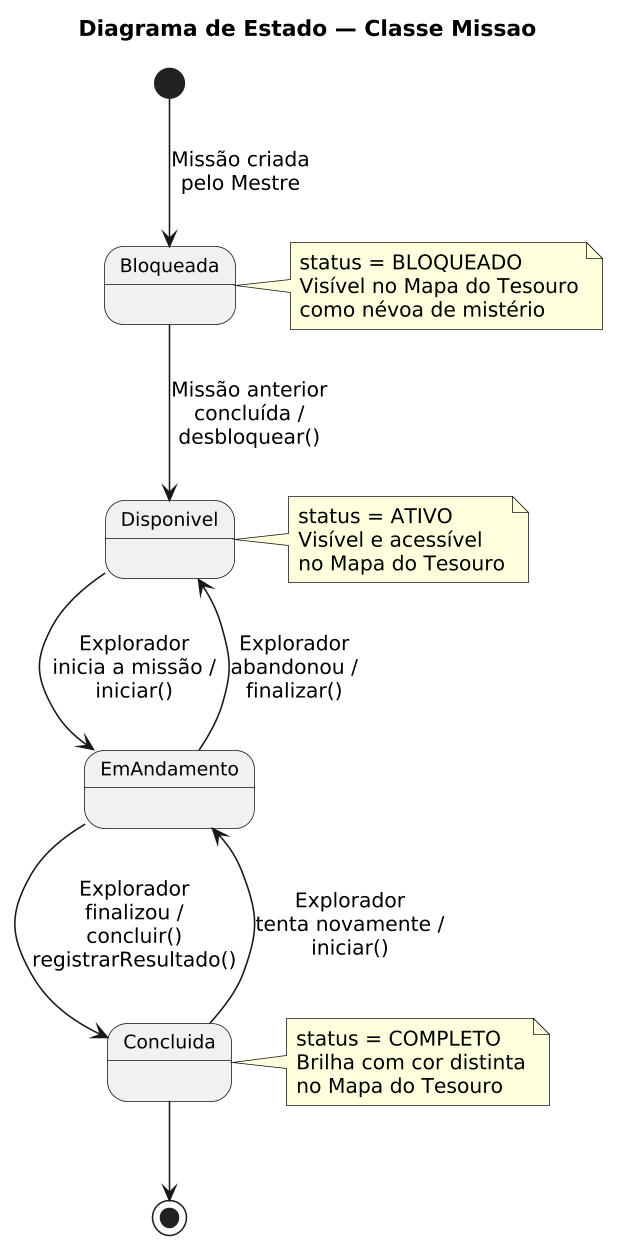
\includegraphics[width=0.75\textwidth]{figuras/est_missao.png}
\end{figure}
 
\subsection{Classe Explorador}
 
O diagrama da Figura~\ref{fig:est_explorador} representa o
ciclo de vida completo de um objeto da classe
\textit{Explorador}. O ciclo tem início quando o Mestre da
Jornada realiza o cadastro do aluno, criando o Perfil do Herói
e gerando a identidade digital — estado \textbf{Cadastrado}.
Em seguida, a credencial é enviada ao responsável e o objeto
transita para \textbf{Aguardando Acesso}, permanecendo neste
estado até que o Explorador realize o primeiro acesso via NFC
ou QR Code e personalize seu avatar, tornando-se \textbf{Ativo}.
 
No estado Ativo, o Explorador pode iniciar missões, transitando
para \textbf{Em Atividade}, onde seus pontos de poder são
atualizados em tempo real. Ao concluir ou abandonar uma missão,
o resultado é registrado e o Diário do Explorador é atualizado,
retornando ao estado Ativo. Períodos prolongados sem acesso
levam o objeto ao estado \textbf{Inativo}, do qual o Explorador
pode retornar ao sistema com histórico e emblemas preservados,
ou ser definitivamente desativado pelo Pedagogo.
 
\begin{figure}[H]
    \centering
    \caption{Diagrama de Estado – Classe Explorador}
    \label{fig:est_explorador}
    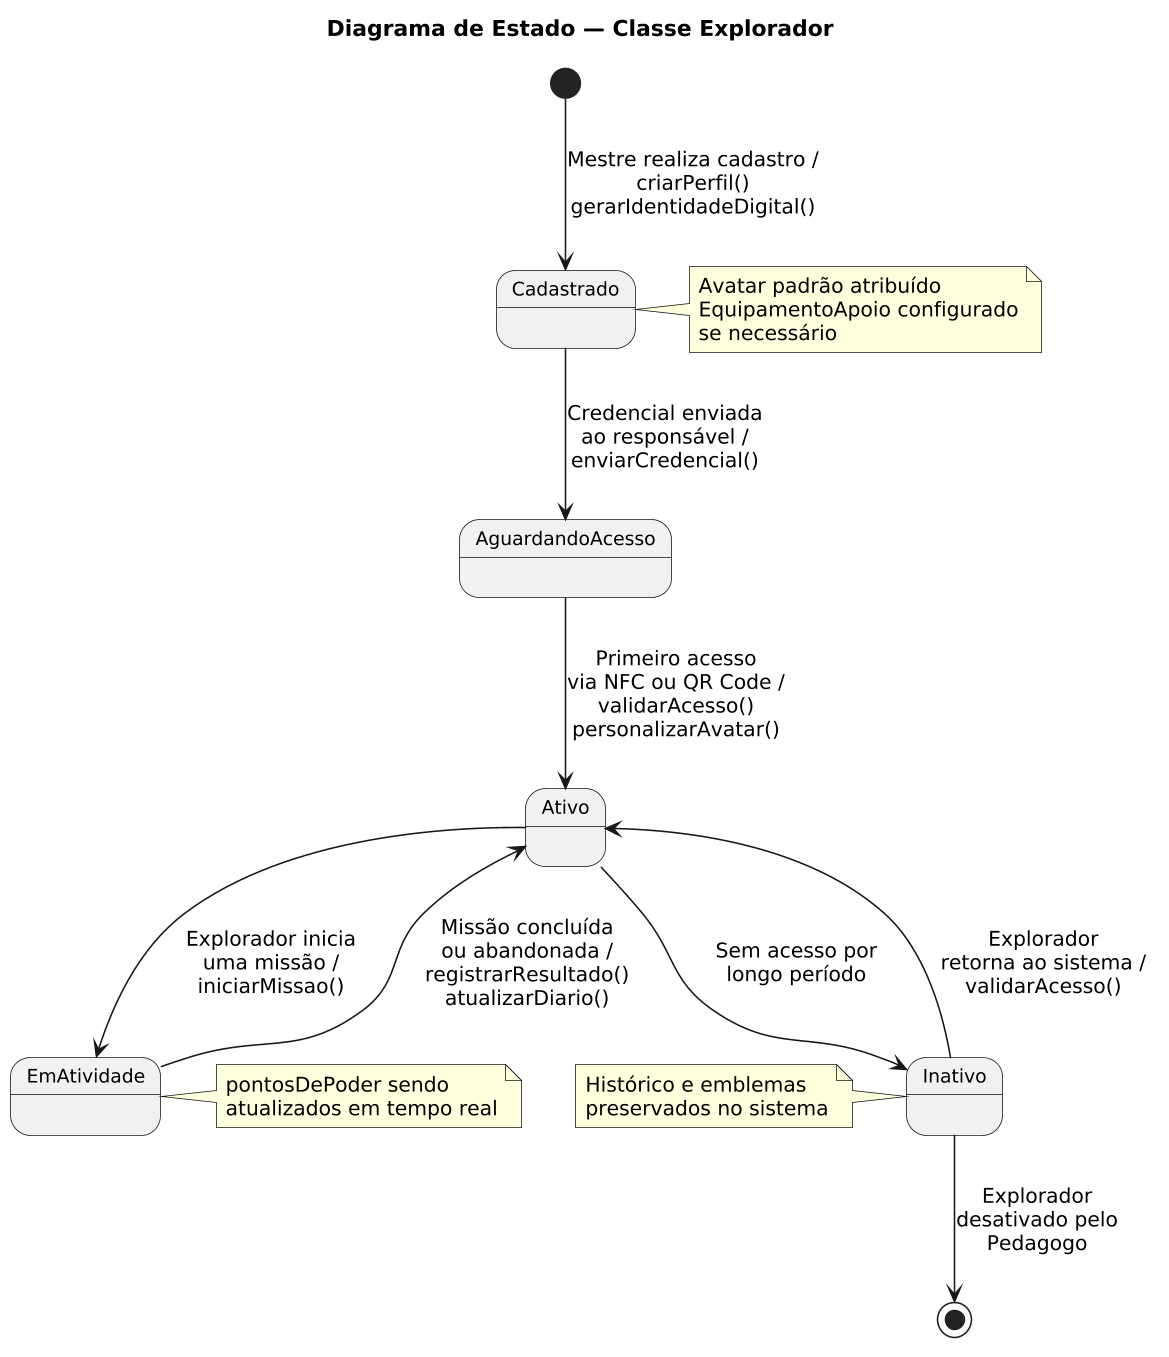
\includegraphics[width=\textwidth]{figuras/est_explorador.png}
\end{figure}
% ============================================================
\section{DECLARAÇÃO DE USO DE INTELIGÊNCIA ARTIFICIAL}
% ============================================================
 
Em conformidade com as diretrizes do Ministério da Educação (MEC) sobre o uso ético e
transparente de ferramentas de Inteligência Artificial (IA) em produções acadêmicas, os
autores declaram que o presente trabalho contou com o apoio de sistemas de IA generativa
em etapas específicas de seu desenvolvimento, devidamente identificadas a seguir.
 
As ferramentas utilizadas foram: \textbf{Figma Make} (prototipação e geração da descrição
completa do sistema), \textbf{Google Gemini} (elaboração dos descritivos técnicos das
interfaces de tela), \textbf{ChatGPT} (OpenAI) (adaptação do diagrama de casos de uso e
geração da árvore de organização do modelo) e \textbf{Claude Sonnet 4.6} (Anthropic)
(geração do código PlantUML dos diagramas de casos de uso e apoio na estruturação do
documento \LaTeX). Em todos os casos, os conteúdos gerados foram revisados, verificados
e adaptados criticamente pelos autores, que assumem integral responsabilidade pelo
resultado final apresentado.
 
As contribuições das ferramentas de IA se concentraram especificamente em:
 
\begin{enumerate}
    \item \textbf{Geração do design do protótipo:} O Figma Make foi utilizado para criar
    as interfaces visuais do sistema, sendo os protótipos apresentados na Seção 2
    resultado dessa ferramenta, posteriormente revisados e ajustados pela equipe.
 
    \item \textbf{Agrupamento de toda a descrição e lógica do sistema:} O Figma Make
    também foi empregado para consolidar a descrição funcional completa do sistema,
    incluindo a definição dos atores, fluxos de navegação e regras de negócio que
    fundamentam a modelagem de casos de uso.
 
    \item \textbf{Melhoria na lógica de correção de atividades:} Ferramentas de IA
    auxiliaram na revisão e aprimoramento das fórmulas de cálculo de nota das
    atividades gamificadas (culinária, quebra-cabeça, jogo da memória), contribuindo
    para torná-las pedagogicamente mais adequadas ao público-alvo do sistema.
\end{enumerate}
 
Ressalta-se que o uso das ferramentas de IA foi subordinado ao julgamento crítico e à
autoria intelectual dos estudantes, em consonância com os princípios de integridade
acadêmica estabelecidos pela instituição. A adoção dessas tecnologias teve caráter
instrumental e não substitui a reflexão, a análise e a tomada de decisão que constituem
o núcleo da aprendizagem na disciplina de Análise e Projeto Orientado a Objetos.
 
\end{document}